\documentclass[10pt,xcolor={usenames},fleqn,mathserif,serif]{beamer}
%%%Usefull link
%tikz-equations:
%http://www.wekaleamstudios.co.uk/posts/creating-a-presentation-with-latex-beamer-equations-and-tikz/
\hypersetup{pdfpagemode=FullScreen}
%% colors
\definecolor{bittersweet}{rgb}{1.0, 0.44, 0.37}
\definecolor{brilliantlavender}{rgb}{0.96, 0.73, 1.0}
\definecolor{antiquefuchsia}{rgb}{0.57, 0.36, 0.51}
\definecolor{violetw}{rgb}{0.93, 0.51, 0.93}
\definecolor{Veronica}{rgb}{0.63, 0.36, 0.94}
\definecolor{atomictangerine}{rgb}{1.0, 0.6, 0.4}
\definecolor{darkgray}{rgb}{0.66, 0.66, 0.66}
\definecolor{brightcerulean}{rgb}{0.11, 0.67, 0.84}
\definecolor{cadmiumorange}{rgb}{0.93, 0.53, 0.18}
\definecolor{ochre}{rgb}{0.8, 0.47, 0.13}
\definecolor{midnightblue}{rgb}{0.1, 0.1, 0.44}
\definecolor{lemon}{rgb}{1.0, 0.97, 0.0}
\definecolor{grey}{rgb}{0.7, 0.75, 0.71}
\definecolor{amber}{rgb}{1.0, 0.75, 0.0}
\definecolor{almond}{rgb}{0.94, 0.87, 0.8}
\definecolor{bf}{RGB}{88, 86, 88}
\definecolor{bb}{RGB}{177, 177, 177}
%%%%%%%%%%%%%%%%%%%%%%%%%%%%%%%%%%% importa pacchetti
\usepackage{usepkg}
%%%%%%%%%%%%%%%%%%%%%%%%%%%%%%%%%%% Funzioni generali
\usepackage{functions}
%http://tex.stackexchange.com/questions/246/when-should-i-use-input-vs-include
\newcommand{\setmuskip}[2]{#1=#2\relax} %%problem usinig mu with calc (req by mathtools) loaded
\usepackage{sources}
%\usepackage{length}
%%%%%%%%%%%%%%%%%%%%%%%%%%%%%%%%%%% Funzioni per questo file main
\usepackage{mathOp}
\usepackage{beamersetup}
\def\status{coazione}
\def\keeptrying{coazione}
\usepackage{LocalF}
%%%%%%%%%%%%%%%%%%%%%%%%%%%%%%%%%
\title{Risonanza magnetica nucleare}
% A subtitle is optional and this may be deleted
\subtitle{Risonanza magnetica nucleare}
\date{NOW, \today}
% - Either use conference name or its abbreviation.
% - Not really informative to the audience, more for people (including
%   yourself) who are reading the slides online
% Let's get started
\begin{document}

\addtobeamertemplate{block begin}{\setlength\abovedisplayskip{2pt}\setlength\belowdisplayskip{2pt}\setlength\abovedisplayshortskip{2pt}\setlength\belowdisplayshortskip{2pt}}

\addtobeamertemplate{block begin}{\vspace*{-3pt}}{}
\addtobeamertemplate{block end}{}{\vspace*{-3pt}}

\begin{frame}
  \titlepage
\end{frame}

\begin{frame}{tempo interno per}
\tableofcontents[onlyparts]
\end{frame}

% Section and subsections will appear in the presentation overview
% and table of contents.
%\frame{\tableofcontents[onlyparts]}
%\begin{frame}{Argomenti}
%  \tableofcontents[part=1,hideallsubsections%,pausesections
%  ]
%  % You might wish to add the option [pausesections]
%\end{frame}

\part{Intro}\linkdest{intro}

\begin{frame}[label={why}]{Why?}
Cardiologo: adesso non riesco a trovare essere me - il mio nemico \'e il sonno - workout condizione stanchezza (l'autunno/inverno scorso passato a pensare di fare e essere coazione).
Uso del tempo sempre come 2 giorni prima dell'esame.
Come essere me? Capitalit\'a progetto
obiettivo? workout me

\end{frame}

\begin{wordonframe}{Cosa provo?}
Angoscia insopprimibile: essenza me nella dipendenza
Abitudine me ''pensare''
Cosa provo mentre ascolto Tosetti che legge la presentazione?
Cosa provo nel malessere dietro il magnete?
Cosa provo quando devo iniziare a fare qualcosa?
Quando non faccio in tempo a fare le cose che dovrei: 
\end{wordonframe}

\part{NMR blowing}
\begin{frame}[allowframebreaks]{Reg Lez}

\begin{itemize}
  

\item 

\end{itemize}

\end{frame}

\part{Succo}\linkdest{succo}
\begin{frame}{Induced fem in coil due to spinning M}
\begin{align*}
&emf=-\TDof{t}\int d^3r\vec{M}(\vec{r},t)\cdot\vec{\mathcal{B}}_{rec}\\
&S\propto \frac{\gamma^3B_0^2\rho_0}{T}
\end{align*}
\begin{figure}[!ht]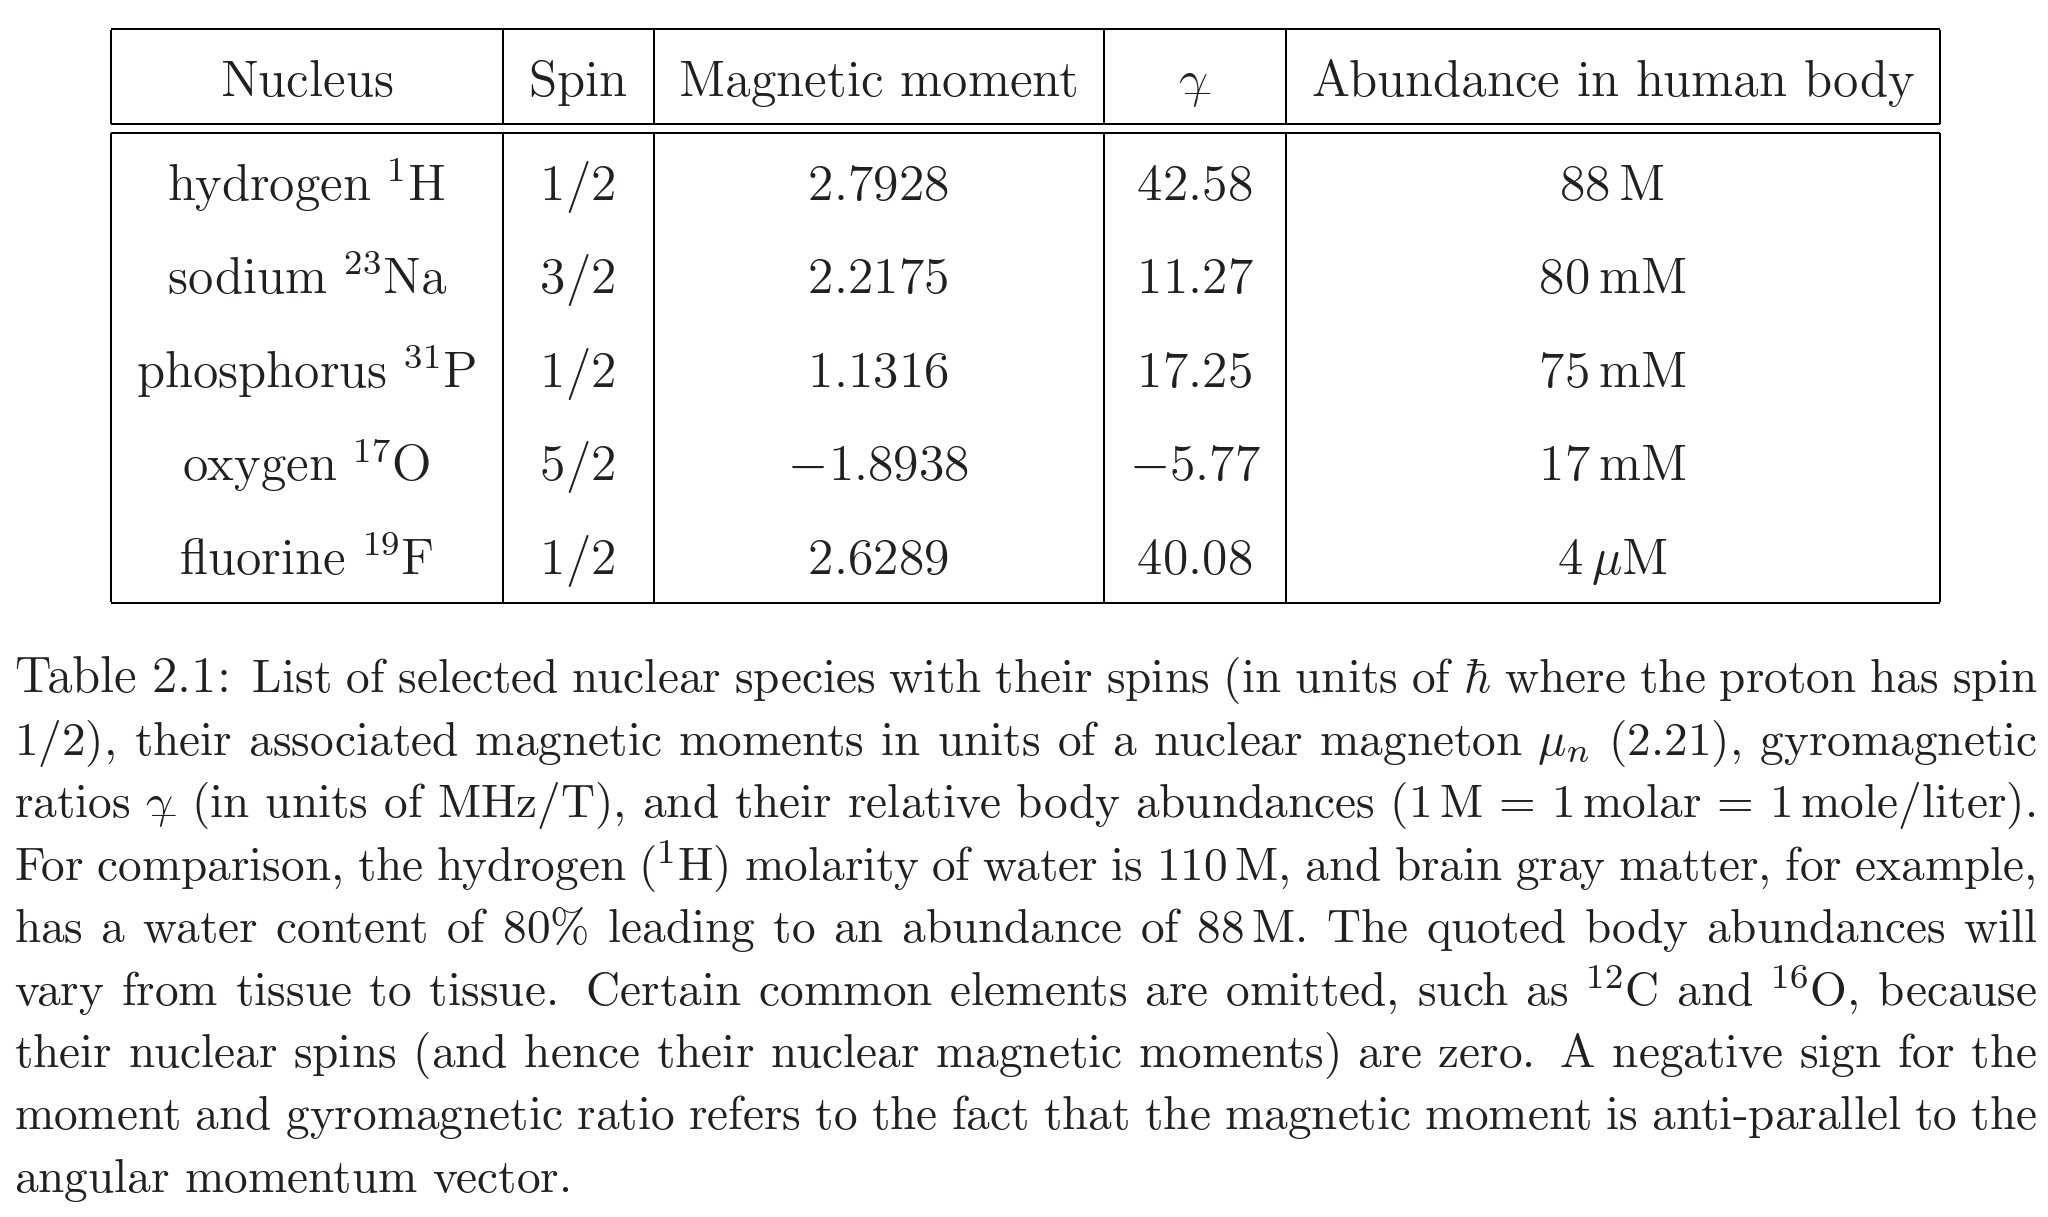
\includegraphics[trim={0cm 0cm 0 0},clip, keepaspectratio,width=0.5\textwidth]{nuclei}\label{fig:nuclei}\end{figure}
\end{frame}

\begin{frame}{On-resonance condition}
    Per $\omega=\omega_0$:
\begin{align*}
&(\TDy{t}{\vec{\mu}})'=\omega_1\vec{\mu}\wedge\hat{x}'
\end{align*}
Flip-angle: $\Delta\theta=\gamma B_1\tau$
\end{frame}

\begin{frame}{Equazione di Block}
$T_2*=T_2+T_2$: se domina $T_2'$ dovuto a disomogeneit\'a compo magnetico esterno $\magort{}$ pu\'o essere rifasata.
Interazioni spin-lattice: $T_1$.
\begin{align*}
&\TDy{t}{M_z}=\frac{(M_0-M_z)}{T_1}\\
&M_z(t)=M_z(0)\exp{-\frac{t}{T_1}}+M_0(1-\exp{-\frac{t}{T_1}})
\end{align*}
Local field variation: dephasing $T_2$.
\begin{align*}
&\TDy{t}{\magort}=(\gamma\magort{}\wedge\vec{B}_{ext})_{NR}-\frac{1}{T_2}\magort{}\\
&\magort{}(t)=\magort{}(0)\exp{-\frac{t}{T_2}}
\end{align*}
\end{frame}

\begin{wordonframe}{Magnetismo elettronico}
La maggior parte delle molecole hanno stato fondamentale elettronico $S=L=0$: no momento magnetico. Eccezioni: $\cel{O}{2}{}{}$ con stato fondamentale $S=1$, composti con metalli di transizione, molecole con elettroni dispari.
La maggior parte dei composti sono diamagnetici ($\chi<0$: weak diamagnetis induced by electron orbital current).
Sostanza con momento magnetico in stato fondamentale sono solitamente paramagnetiche ($\chi>0$): se electron magnetic moment interagiscono debolmente \'e possibile EPR-ESR.
(NMR in diamagnetic material: electron magnetism can be ignored because is constant, correzione a campo staticoi)
\end{wordonframe}

\begin{wordonframe}{Kubo: fluctuatuion-dissipation theorem}

\end{wordonframe}

\begin{wordonframe}{Real spectrum FFT: 34-49}
Lorentzian shape-inhomogeneous field broadening-chemical shift(diamagnetic)/spin-spin coupling-J coupling
\end{wordonframe}

\begin{wordonframe}{processi rilassamento spin-spin, spin-lattice}
Lewitt (S dyn): 171-190 nuclear interaction with electric magnetic field (Spin hamiltonian), 543-624 types of relaxation: mechanism, random field relaxation, spectral density, transition probability (dipole-dipole relaxaion: solomon equation, neclear overhauser effectà-)
\end{wordonframe}

\begin{wordonframe}{Nuclear spin interactions}
Spin hamiltonian hypothesis: fast electron motion, low nuclear spin energy.
Nuclear shape, rotation: change in electric/magnetic energies due to orientatio changes.
\end{wordonframe}

\begin{frame}[allowframebreaks]{Free induction decay}

$\pi/2$ pulse lungo $x'$:
\begin{align*}
s(t)\propto\omega_0\int d^3r \exp{-\frac{t}{T_{2}(r)}}B_{\perp}(\vec{r})M_{\perp}(\vec{r},0)\exp{i[(\Omega-\omega(r))t+\phi_0(\vec{r})+\theta_B(\vec{r})]}\\
\phi(\vec{r},t)=-\omega(r)t+\phi_0(\vec{r})=-\gamma B_z(\vec{r})t+\phi_0(\vec{r})
\end{align*}
\begin{figure}[!ht]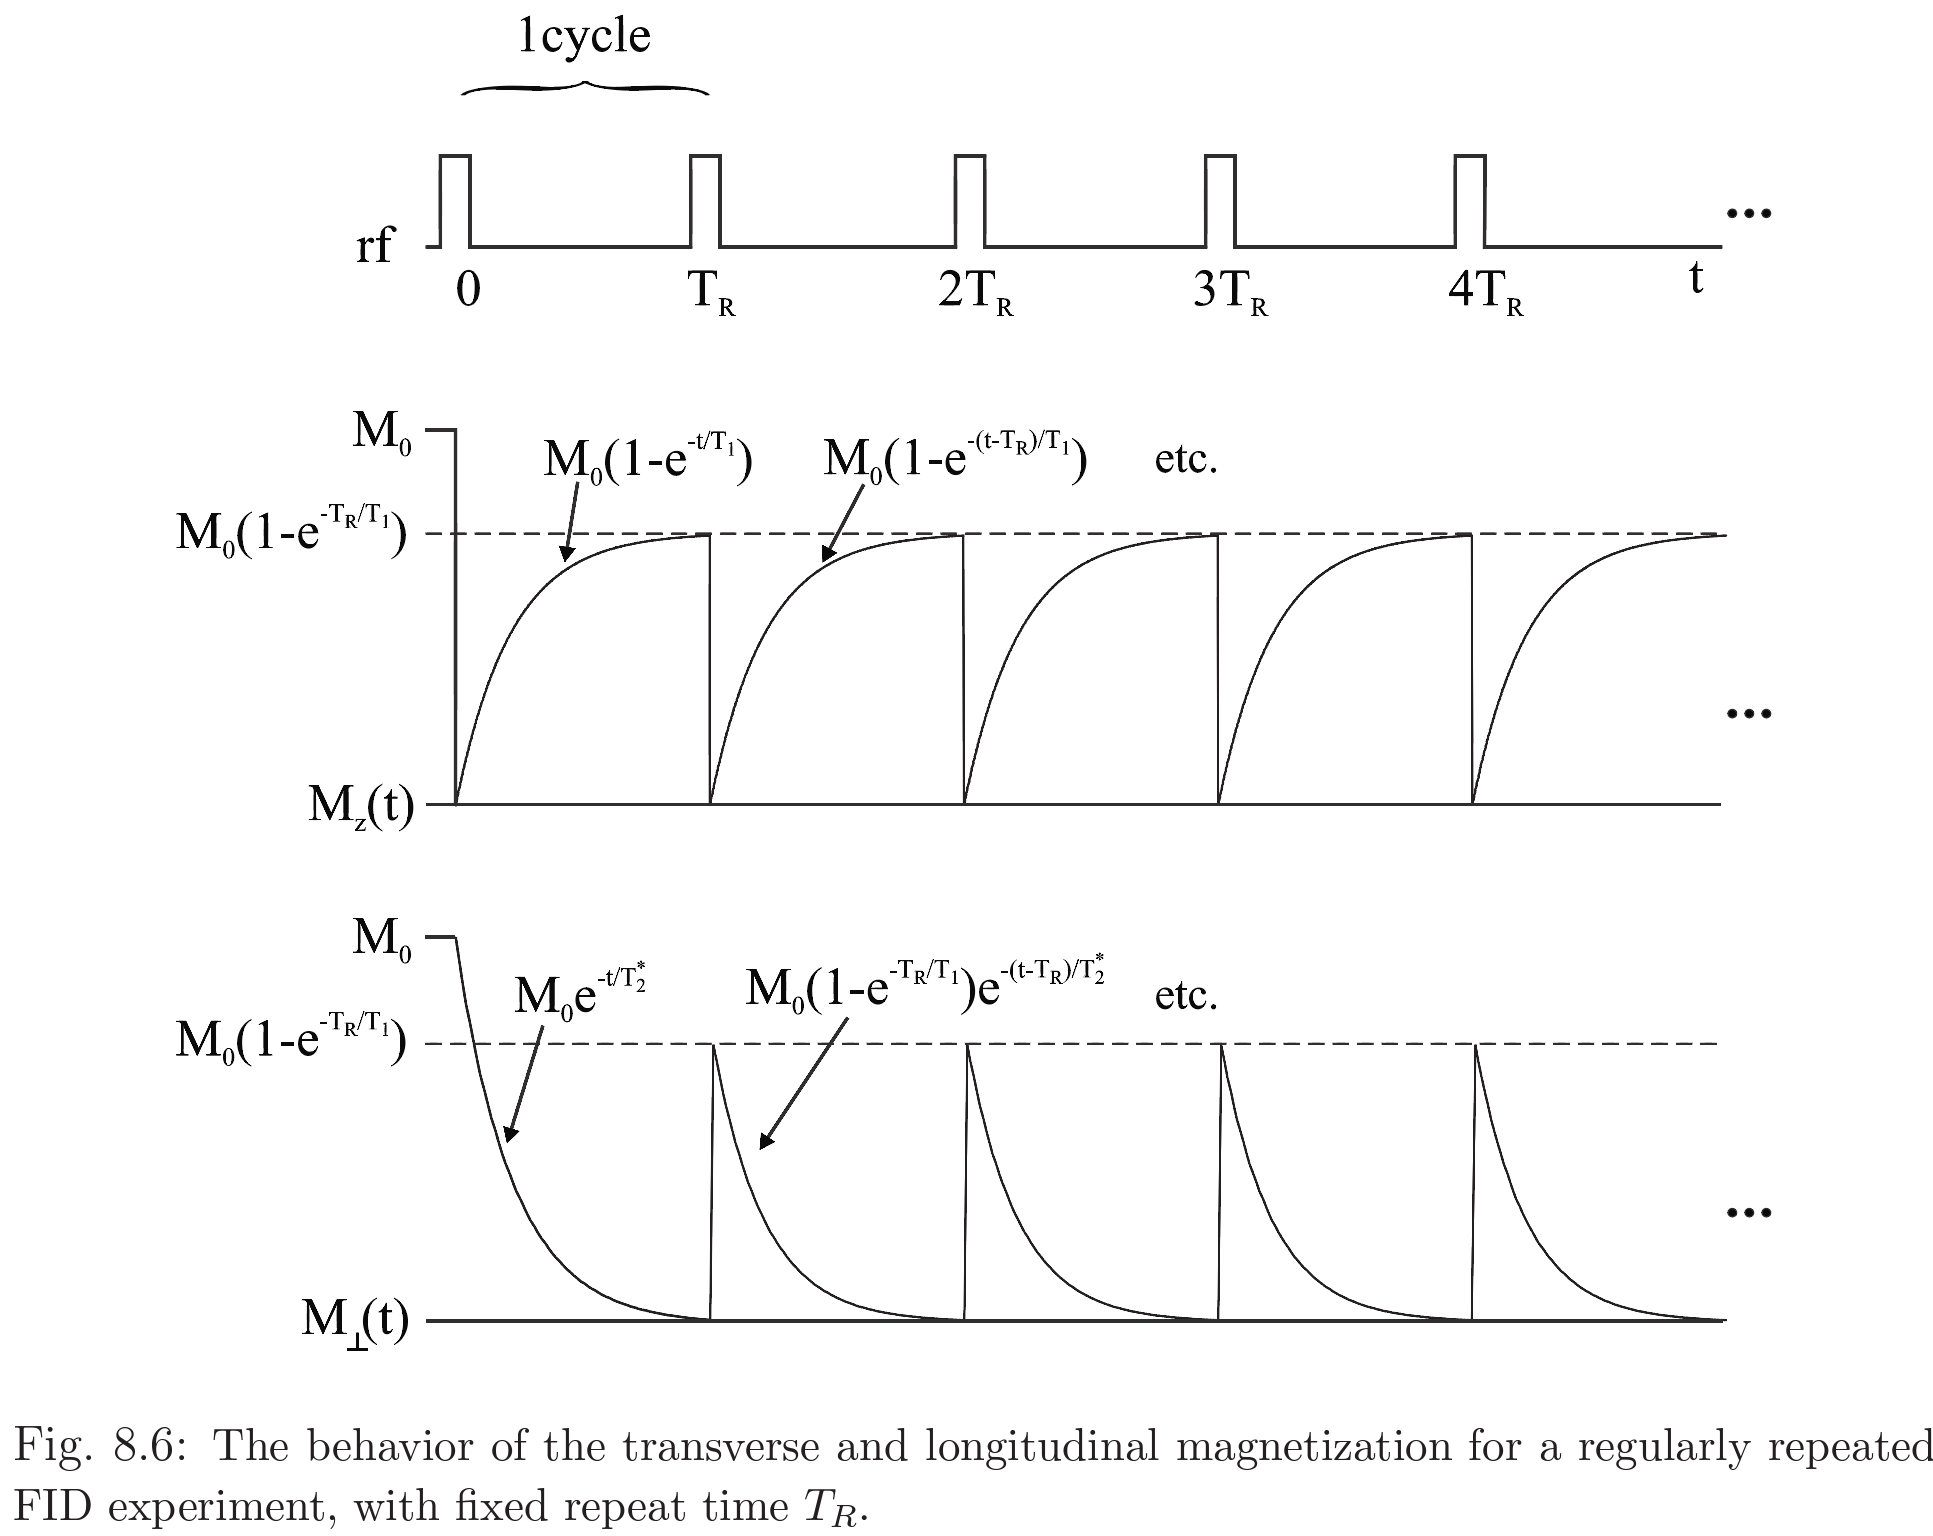
\includegraphics[trim={0cm 0cm 0 0},clip, keepaspectratio,width=0.4\textwidth]{FIDrep}\label{fig:FIDrep}\end{figure}
\begin{align*}
\frac{1}{T_2*}=\frac{1}{T_2}+\frac{1}{T_2'}\\
M_+(\vec{r},t)=M_+(\vec{r},0)\exp{-\frac{t}{T_2*}}\\
\phi(\vec{r},t)=-\gamma[B_0+\Delta B(\vec{r})]t
\end{align*}
\end{frame}

\begin{frame}[allowframebreaks]{Spin-ECHO and $T_2$ measure.}

\begin{figure}[!ht]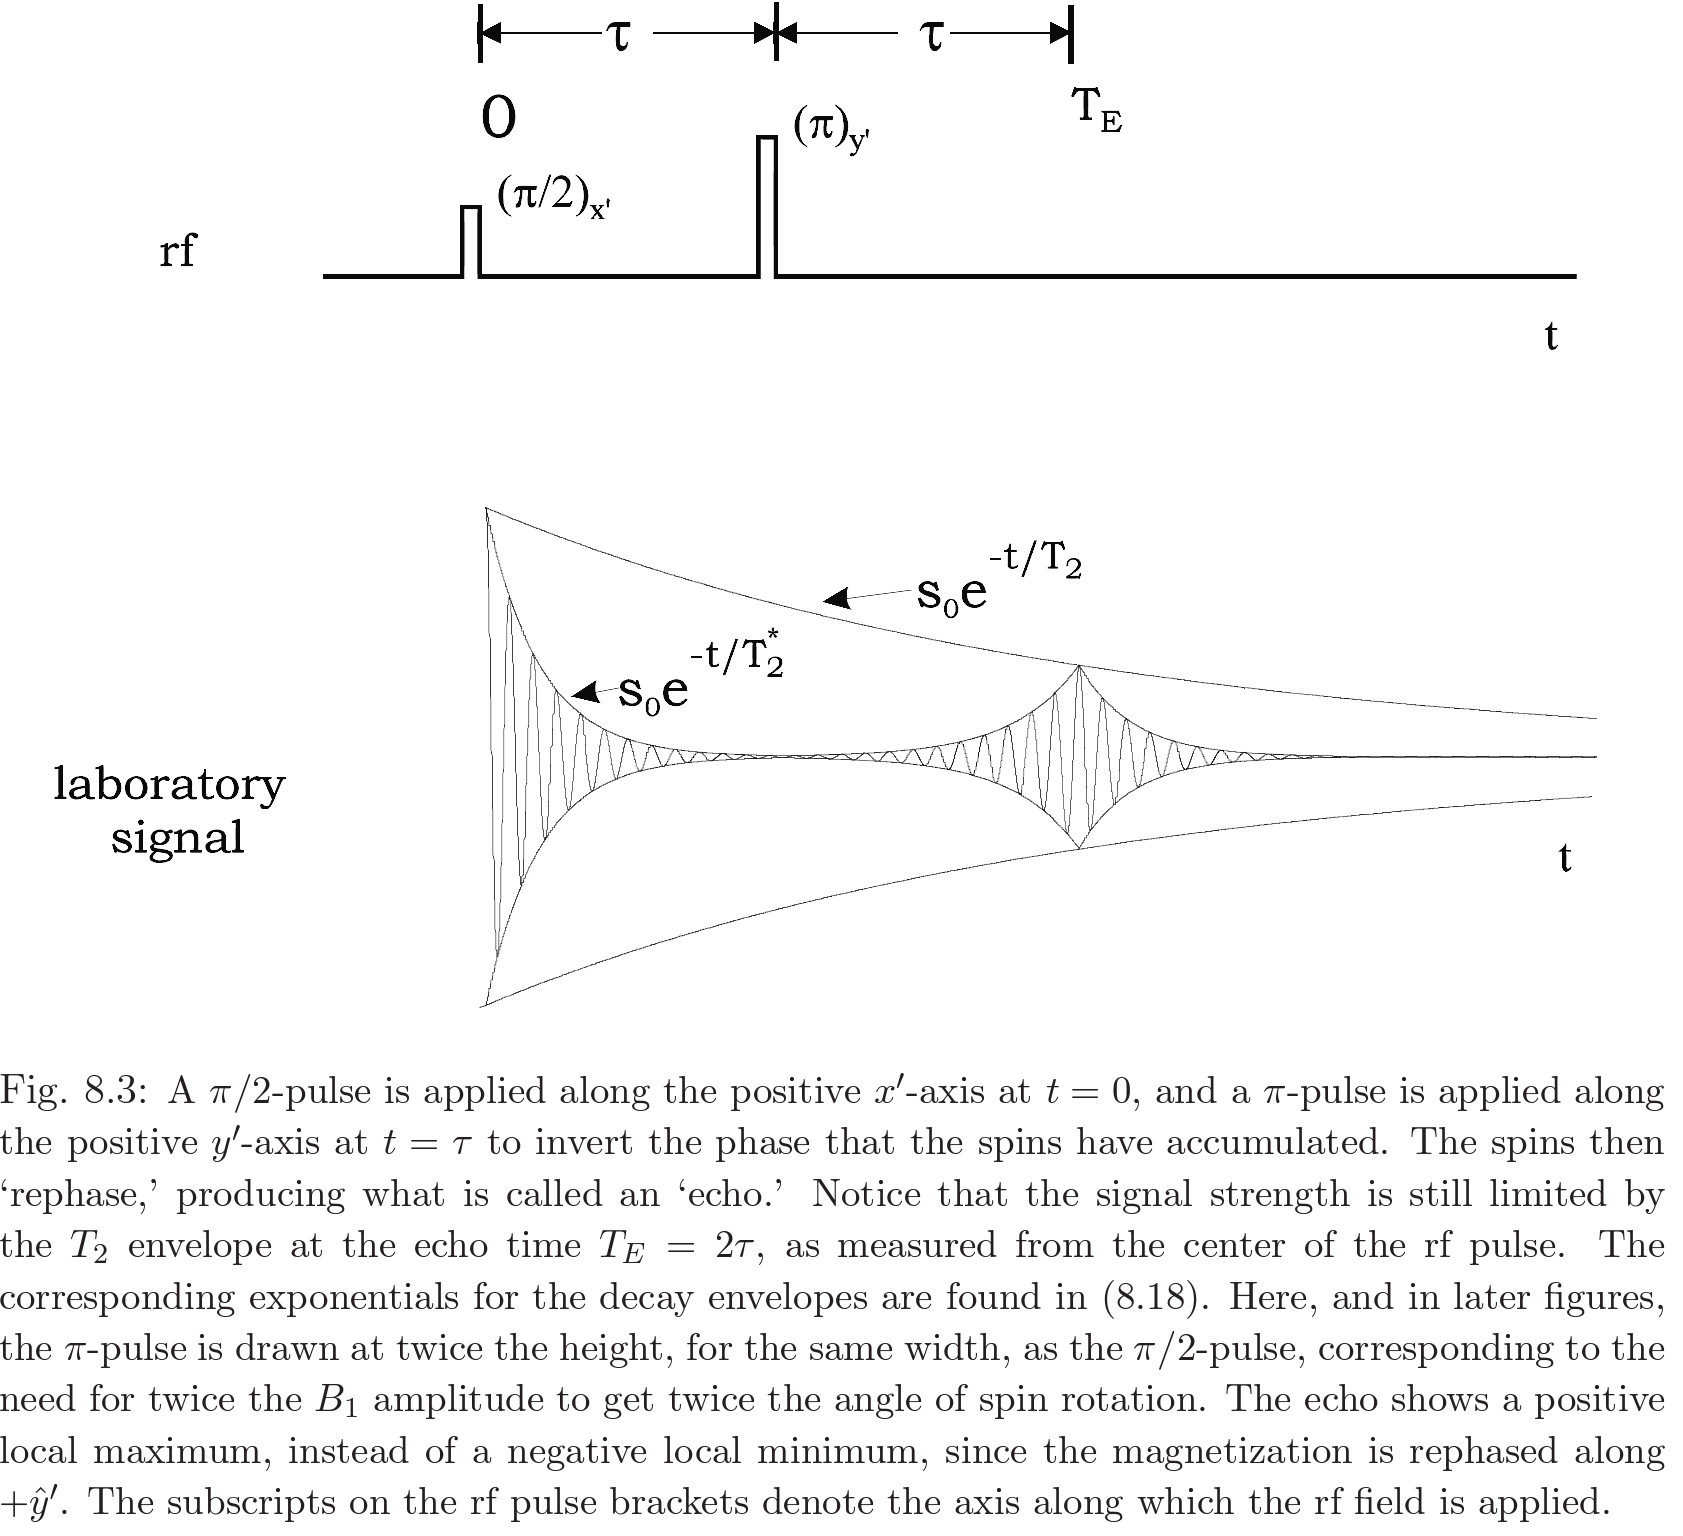
\includegraphics[trim={0cm 0cm 0 0},clip, keepaspectratio,width=0.5\textwidth]{SE}\label{fig:SE}\end{figure}
\begin{figure}[!ht]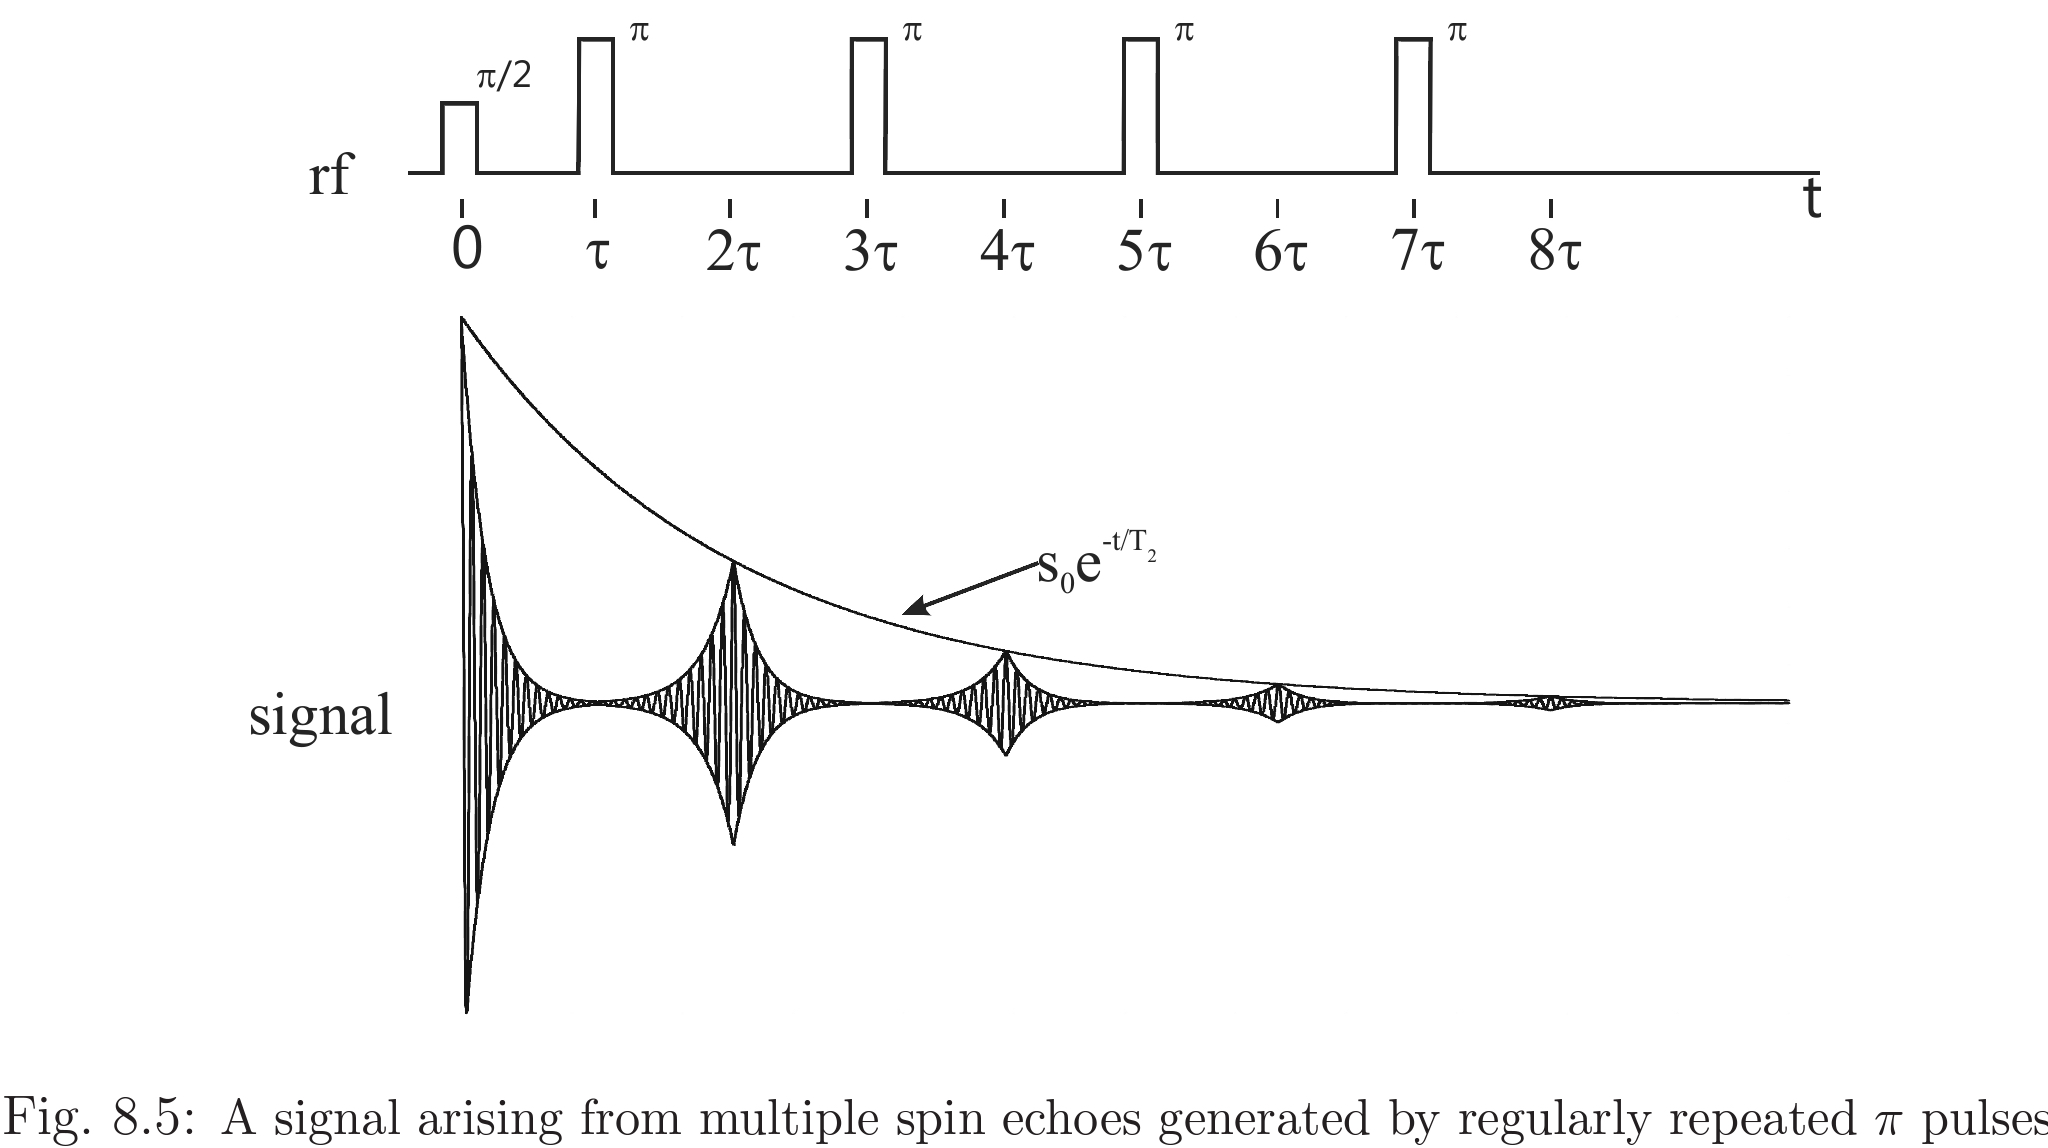
\includegraphics[trim={0cm 0cm 0 0},clip, keepaspectratio,width=\textwidth]{SET2measure}\label{fig:SET2measure}\end{figure}
\begin{align*}
s(T_E)\propto\omega_0\exp{-\frac{T_E}{T_2}}\int d^3 rB_{\perp}M_{\perp}(\vec{r},0)\\
T_2=\frac{T_E'-T_E}{\ln{[s(T_E)/s(T_E')]}}
\end{align*}
\end{frame}

\begin{frame}[allowframebreaks]{Inversion recovery and $T_1$ measure - Spin-echo inversion recovery.}
%succo
Impulso $\pi$ attorno $x'$ e a $T_I$ di $\pi/2$
\begin{align*}
&M_z(0+)=-M_0\\
&M_z(t)=-M_0\exp{-\frac{t}{T_1}}+M_0(1-\exp{-\frac{t}{T_1}})\ 0<t<T_I\\
&\magort{}(t)=|M_0(1-2\exp{-\frac{T_I}{T_1}})|\exp{-\frac{(t-T_I)}{T_2*}}\\
&T_I^{null}=T_1\ln{2}
\end{align*}

\begin{figure}[!ht]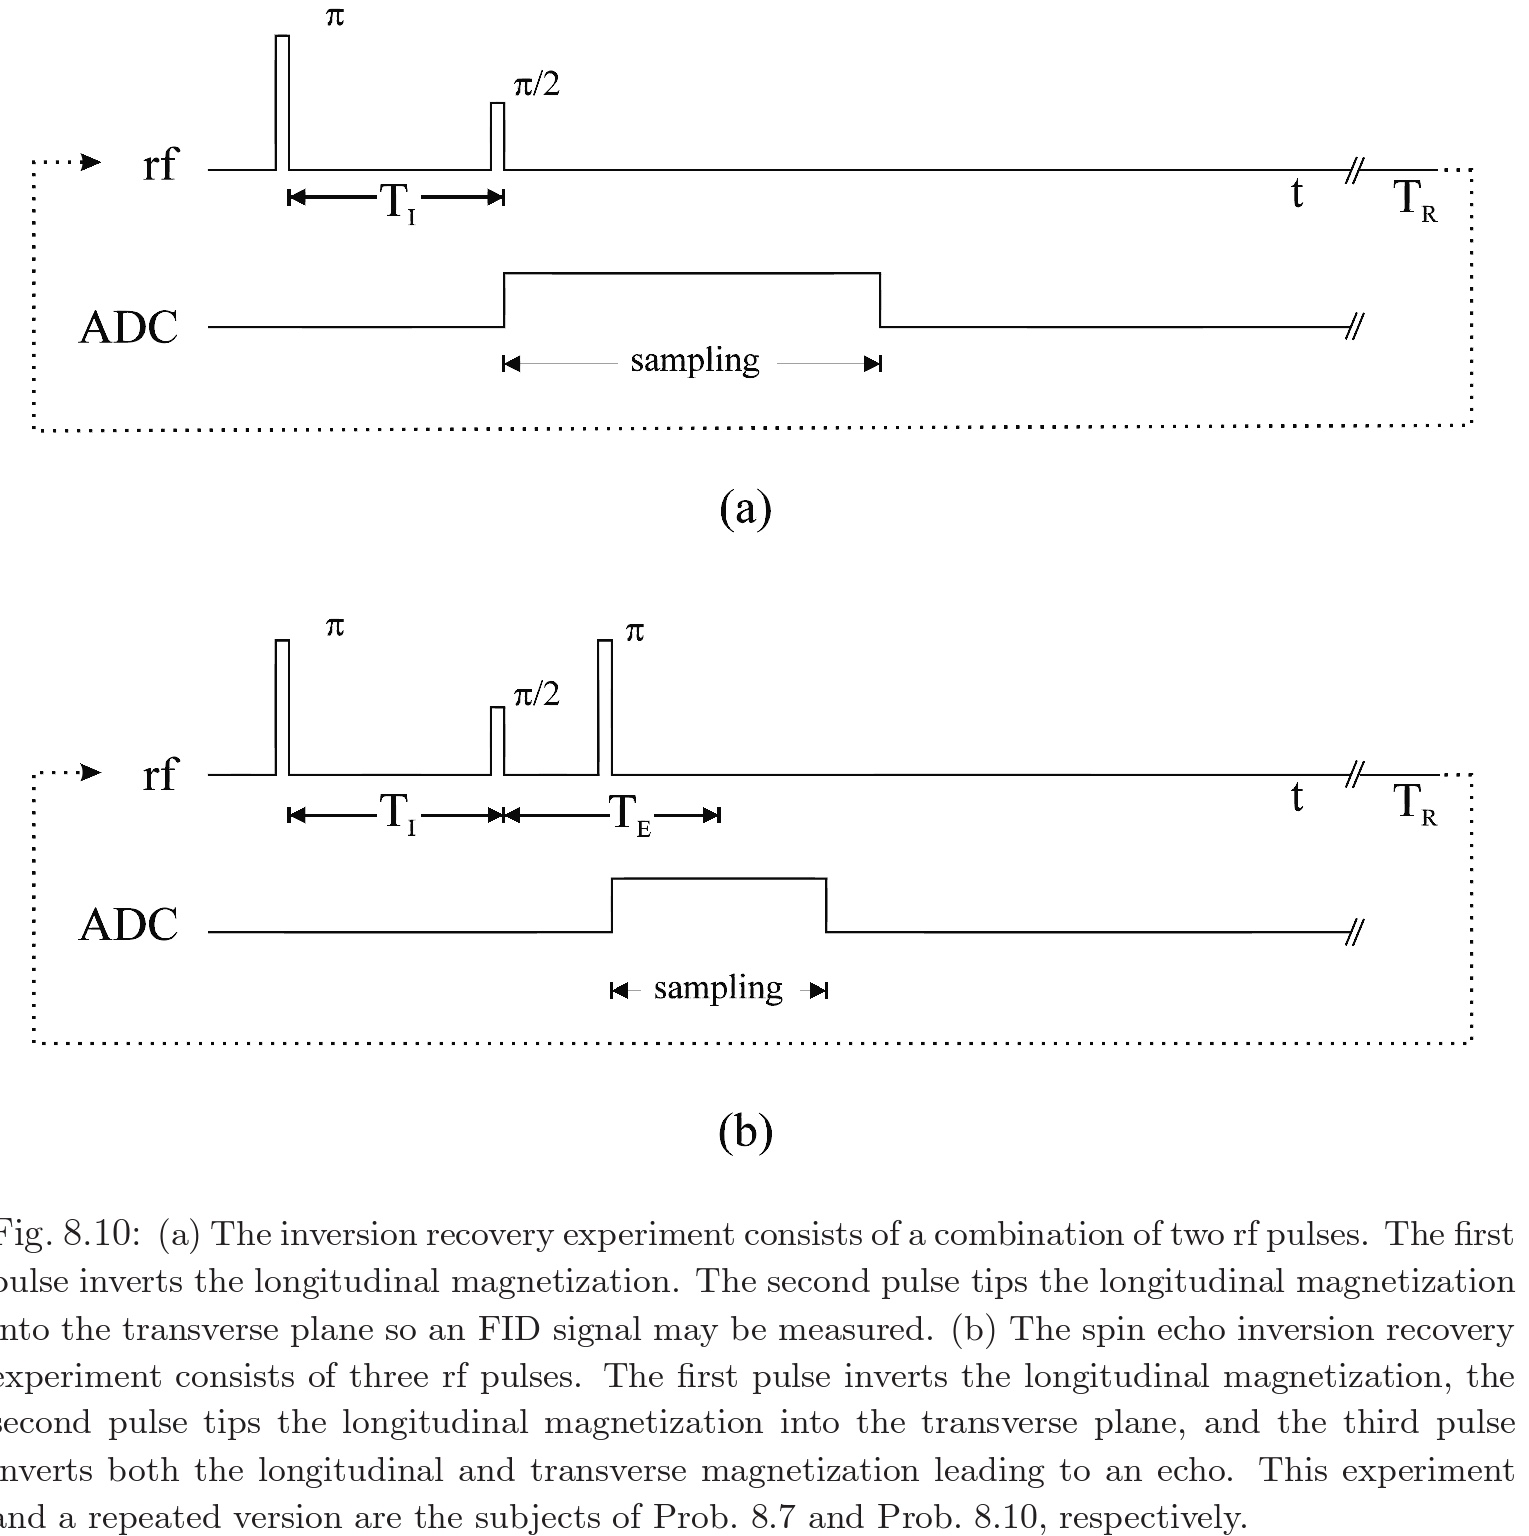
\includegraphics[trim={0cm 0 0 0},clip, width=0.9\textwidth]{IR-SE-sampling}\label{fig:IR-SE-sampling}
\end{figure}

\begin{figure}[!ht]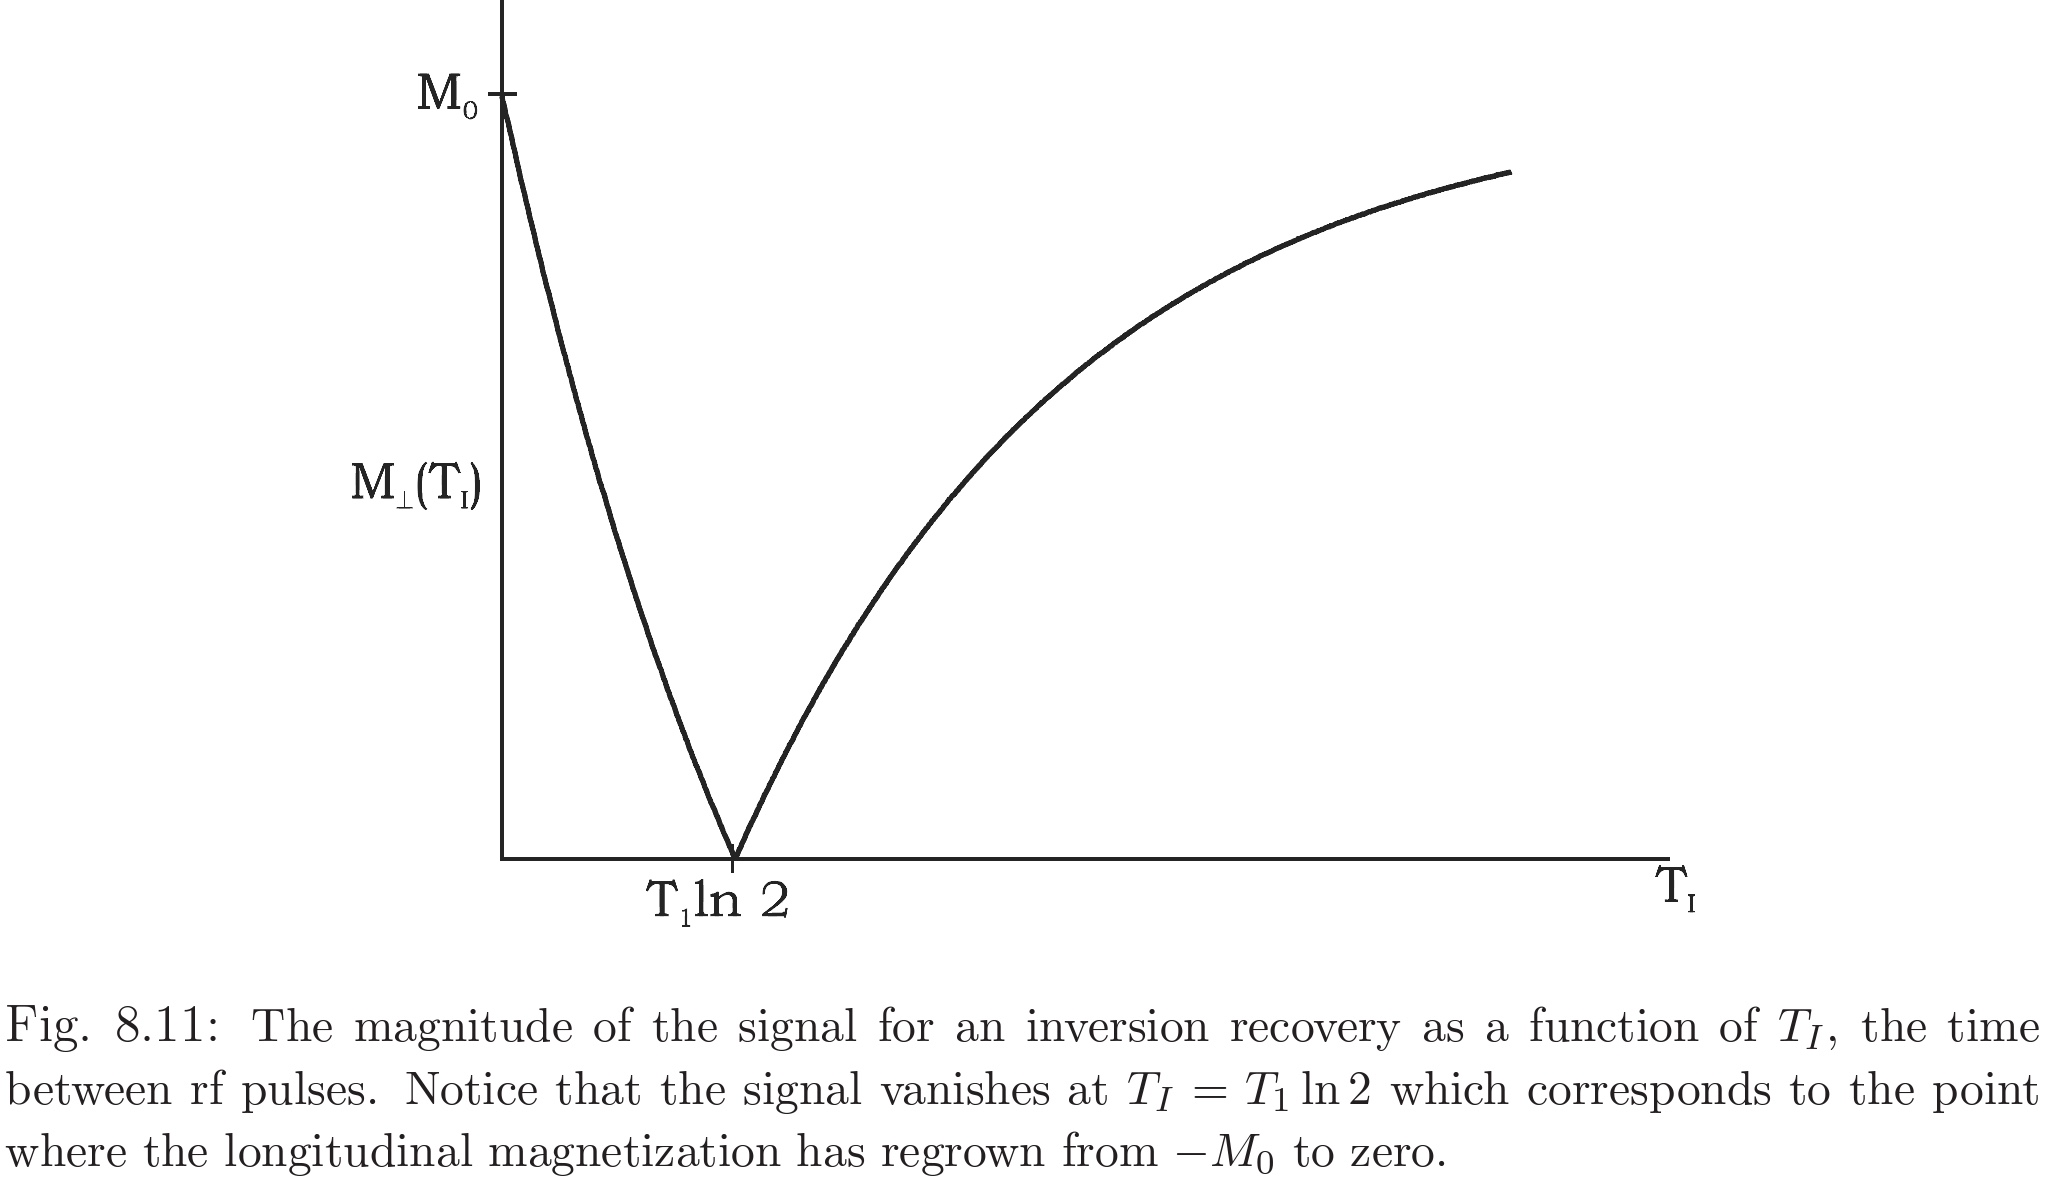
\includegraphics[trim={0cm 0 0 0},clip,width=0.9\textwidth]{IRvsTI}\label{fig:IRvsTI}\end{figure}

\end{frame}

\begin{frame}{Chemical shift and NMR spectroscopy}

Broadband RF excitation: complicated FID signal
\begin{align*}
&\omega_{0i}=\gamma_iB_0
\end{align*}

Shielding constant: linear response of electrons to $B_{ext}$:
\begin{align*}
&B_{shift}(j)=(1-\sigma_j)B_0\to f_{\sigma}=-\sigma\gammabar B_0\\
&s(t)=\sum_jN_j\exp{i\gamma\sigma_jB_0t}
\end{align*}
\end{frame}


\begin{frame}{Fourier imaging}
Aggiungo campo che varia linearmente lungo z:

\begin{align*}
&s(t)\propto\int d^3 r\rho(\vec{r})\exp{i[\Omega t+\phi(\vec{r},t)]}\\
&B_z(z,t)=B_0+zG(t)\ \Rightarrow\ \omega=\omega_0+\omega_G(z,t)
\end{align*}

Frequency encoding: $\omega_G=\gamma zG(t)$.
\begin{equation*}
\phi_G(z,t)=-\int_0^td t'\omega_G(z,t')=-\gamma z\int_0^td t'G(t)
\end{equation*}

1D imaging equation:
\begin{equation*}
s(t)=\int d z\rho(z)\exp{i\phi_G(z,t)}
\end{equation*}
$\rho$ effective spin density.

\end{frame}

\begin{frame}{Gradient echo}
\begin{figure}[!ht]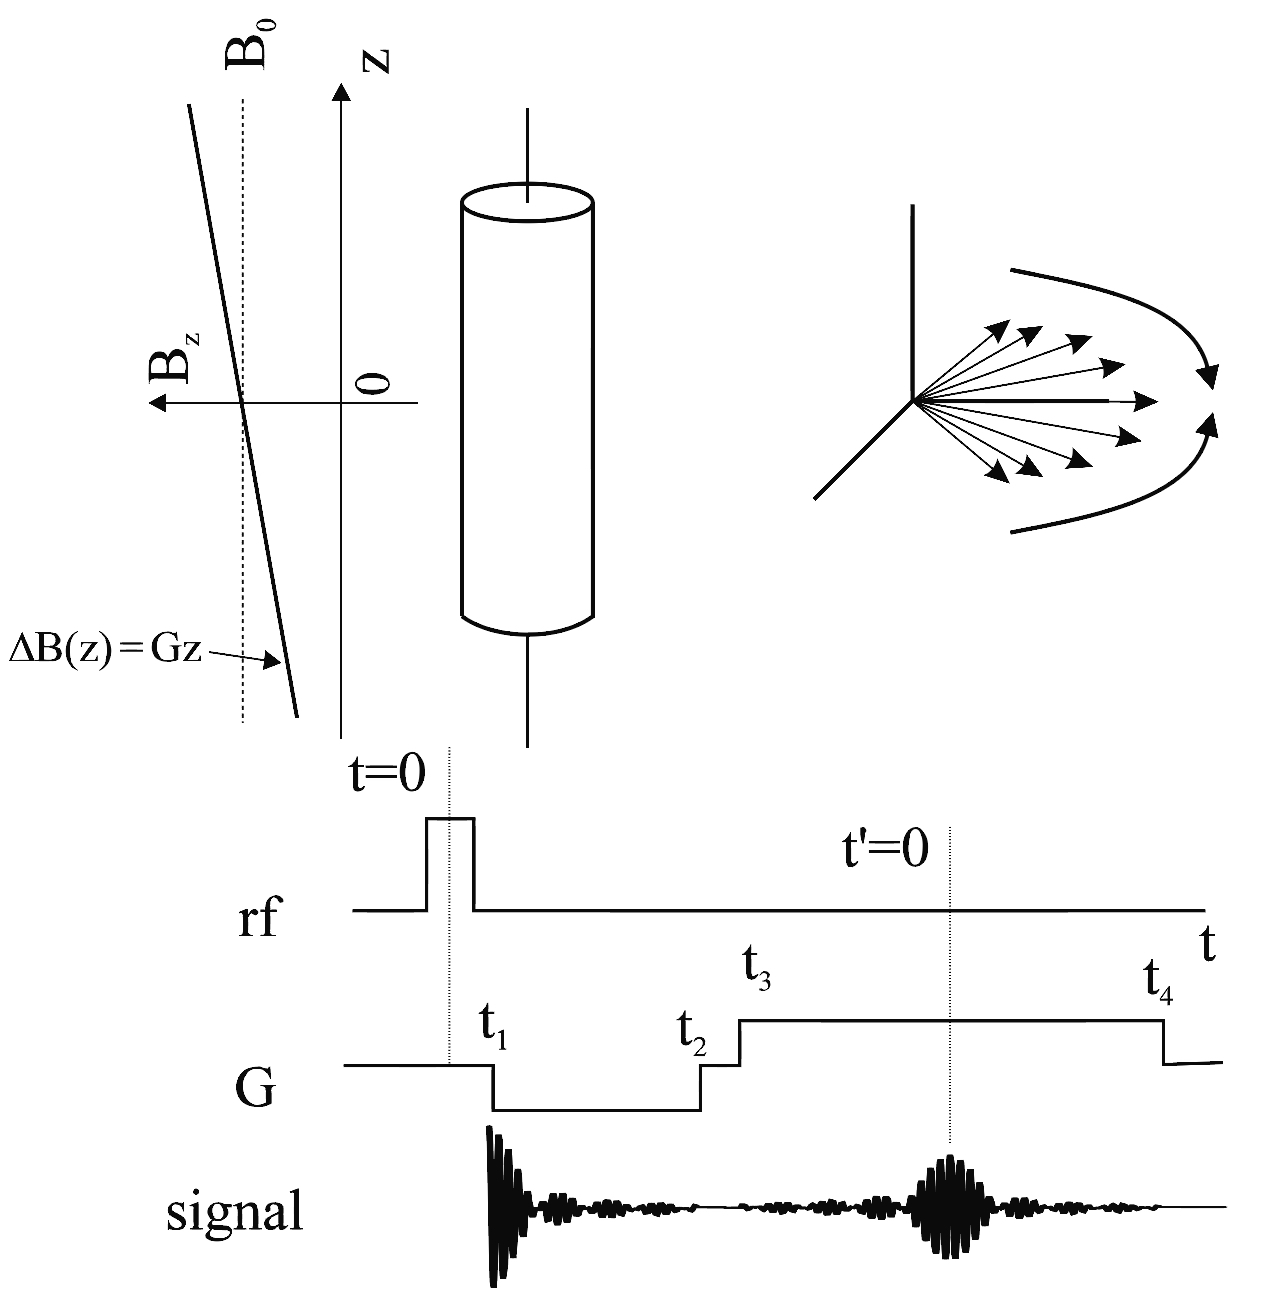
\includegraphics[trim={0cm 0cm 0 0},clip, keepaspectratio,height=0.9\textheight]{GEimaging}\end{figure}
\end{frame}

\begin{frame}[allowframebreaks]{Spin-echo imaging}
\begin{figure}[!ht]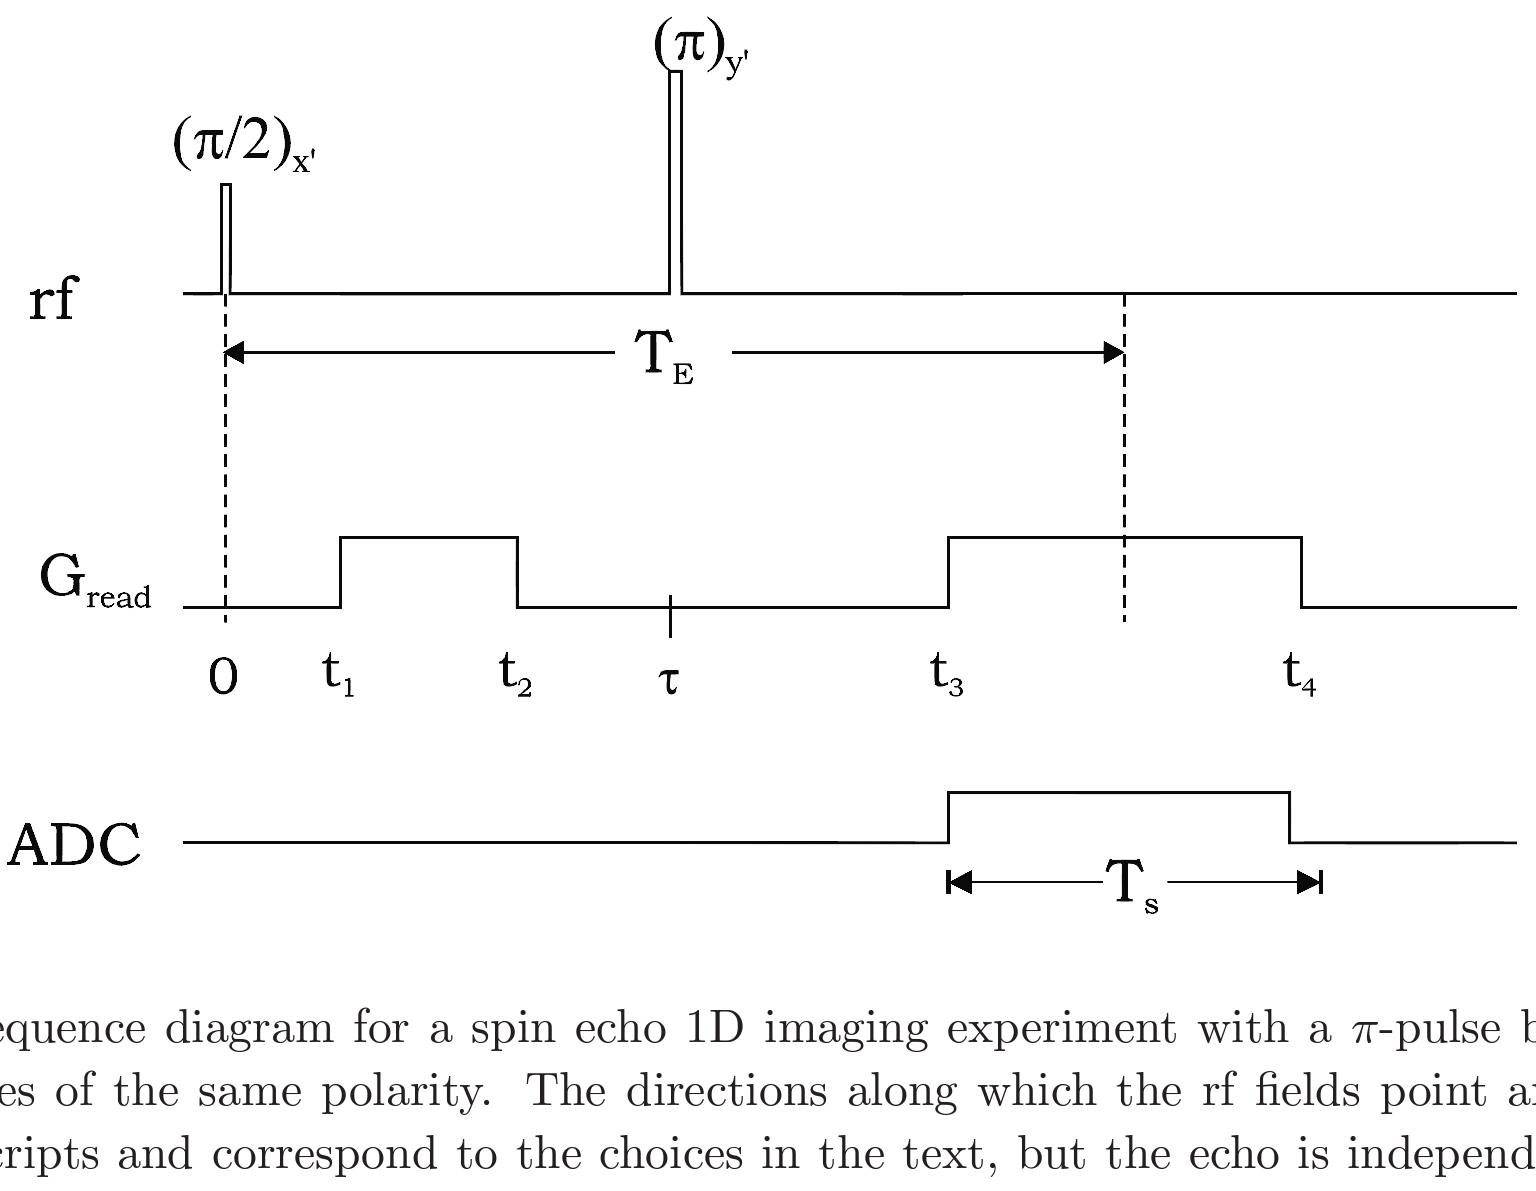
\includegraphics[trim={0cm 0cm 0 0},clip, keepaspectratio,height=0.45\textheight]{SEimaging}\end{figure}
\begin{figure}[!ht]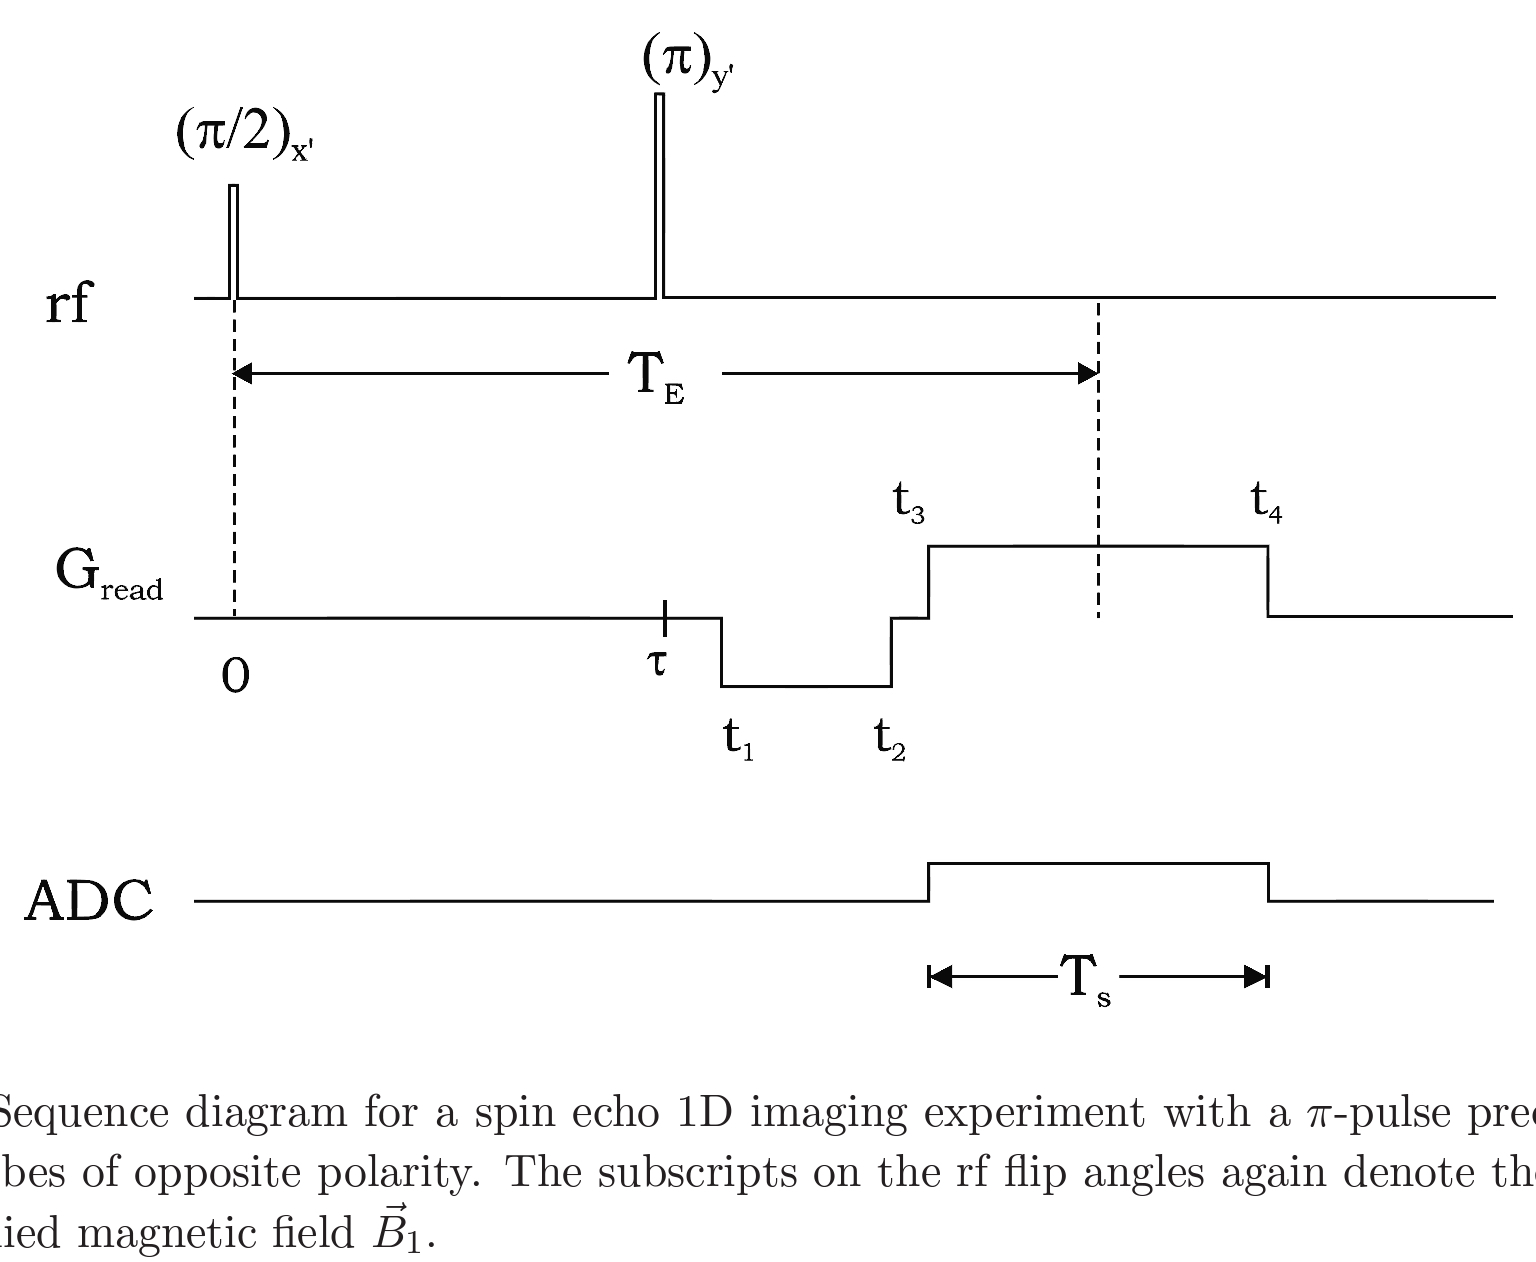
\includegraphics[trim={0cm 0cm 0 0},clip, keepaspectratio,height=0.45\textheight]{SEtotimaging}\end{figure}
\end{frame}

\begin{frame}[allowframebreaks]{Imaging in 3D: 3D imaging  vs 2D multislice imaging}
3D imaging:
\begin{figure}[!ht]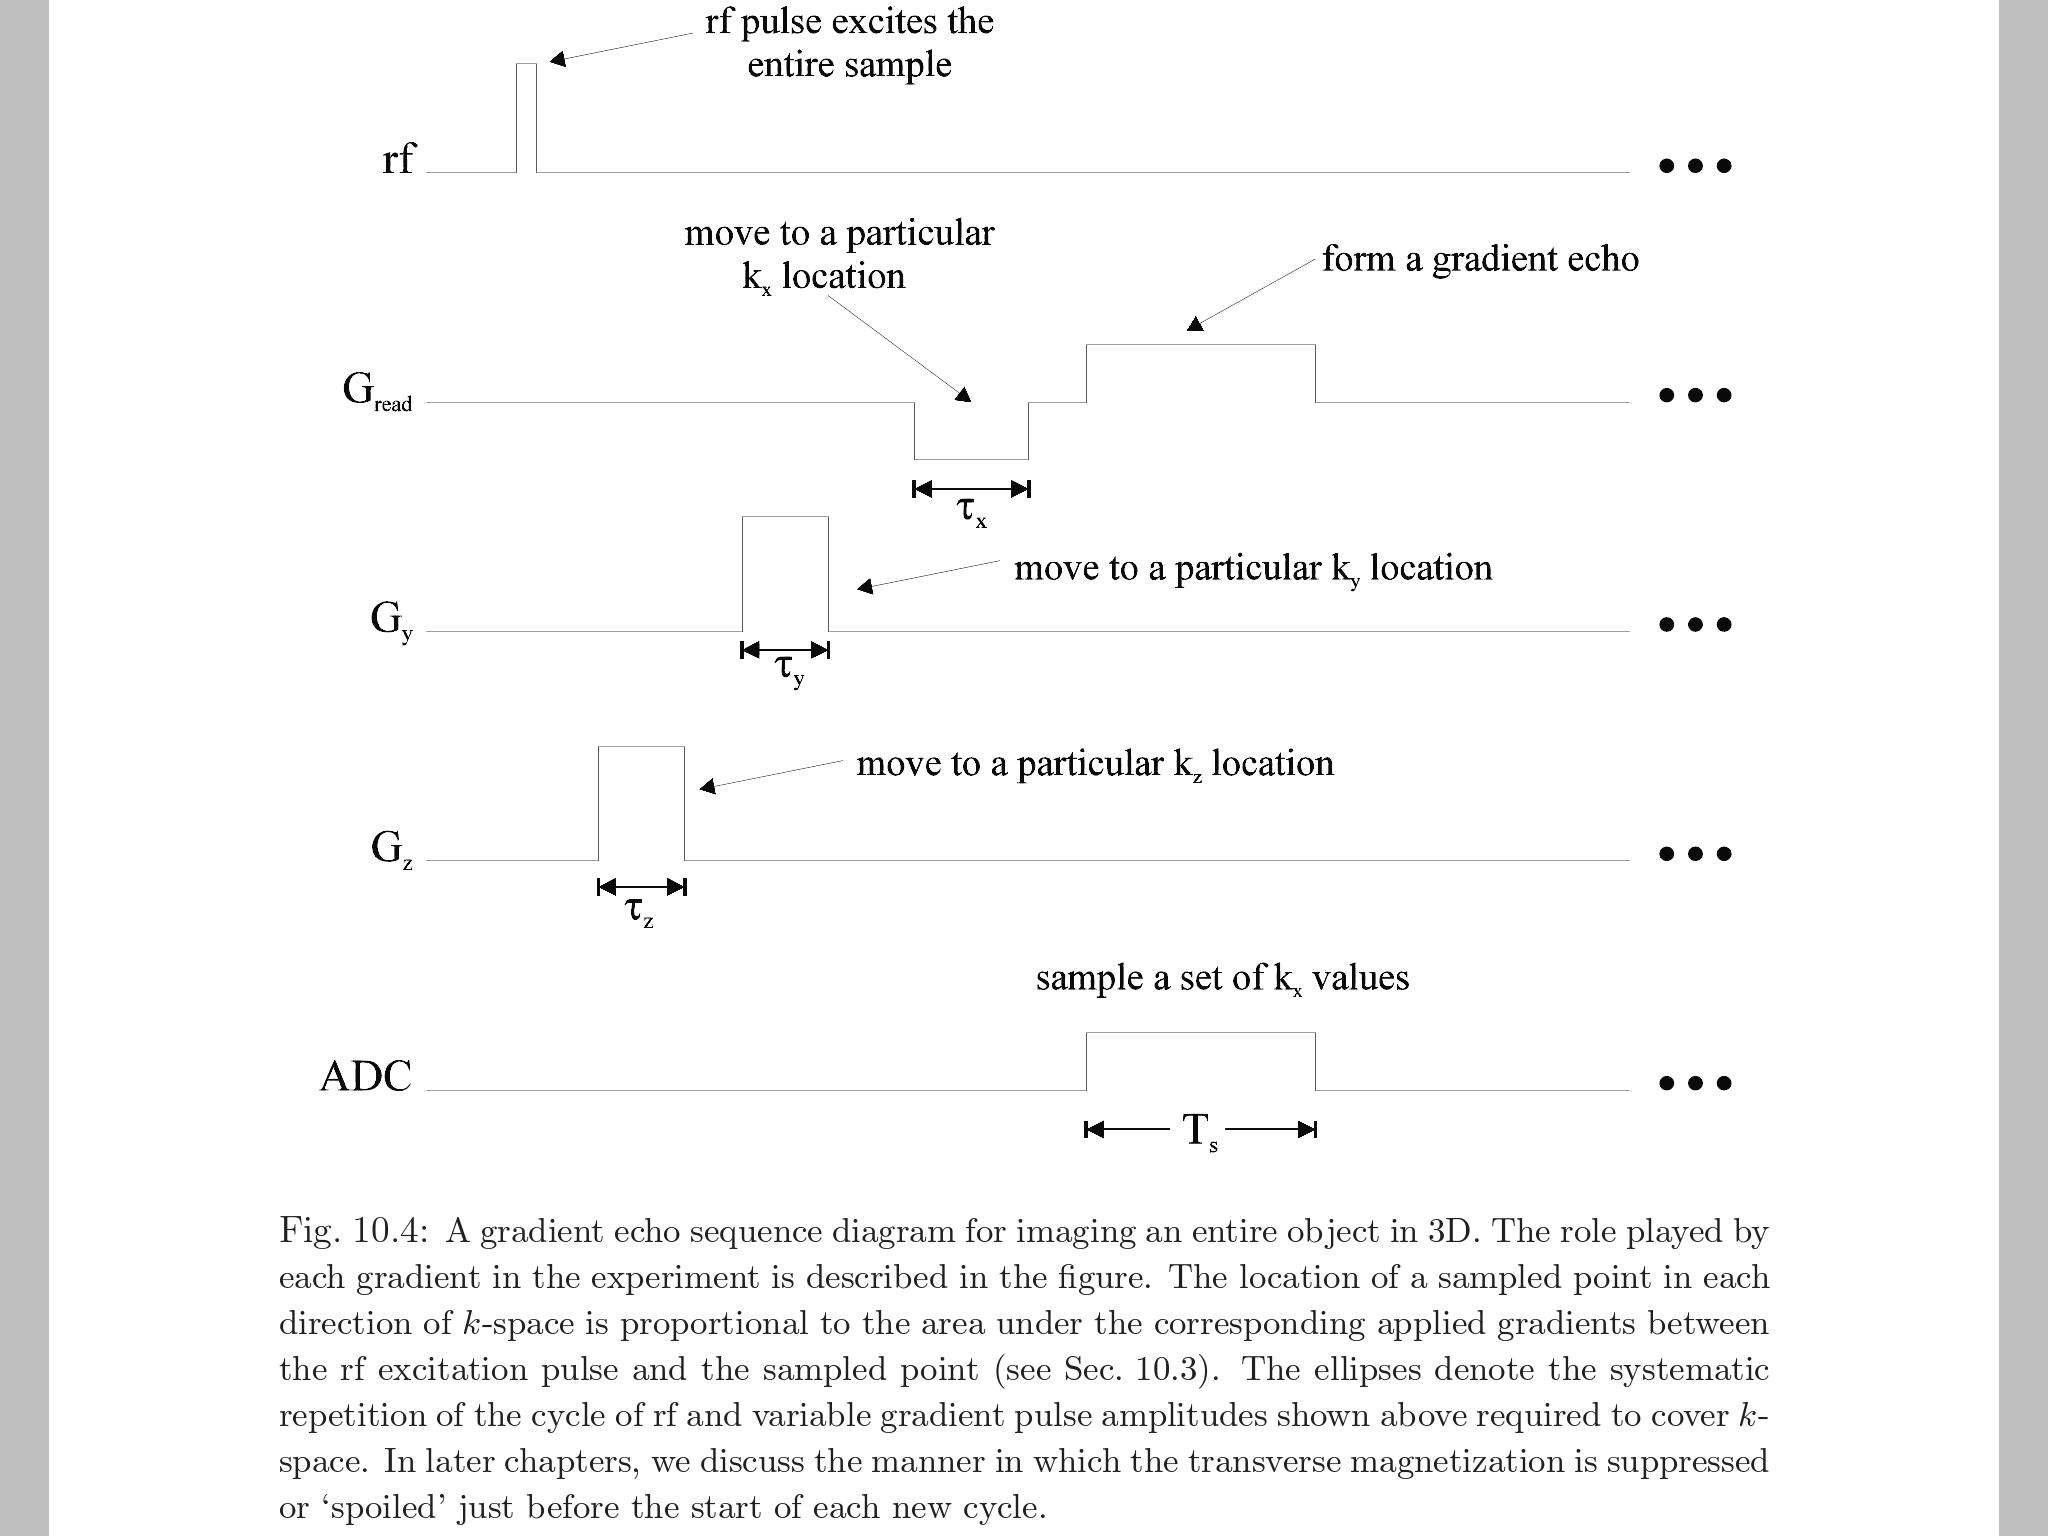
\includegraphics[trim={0cm 0cm 0 0},clip, keepaspectratio,height=0.5\textheight]{3Dimaging}\label{fig:3Dimaging}\end{figure}

2D multi-slice imaging:
\begin{figure}[!ht]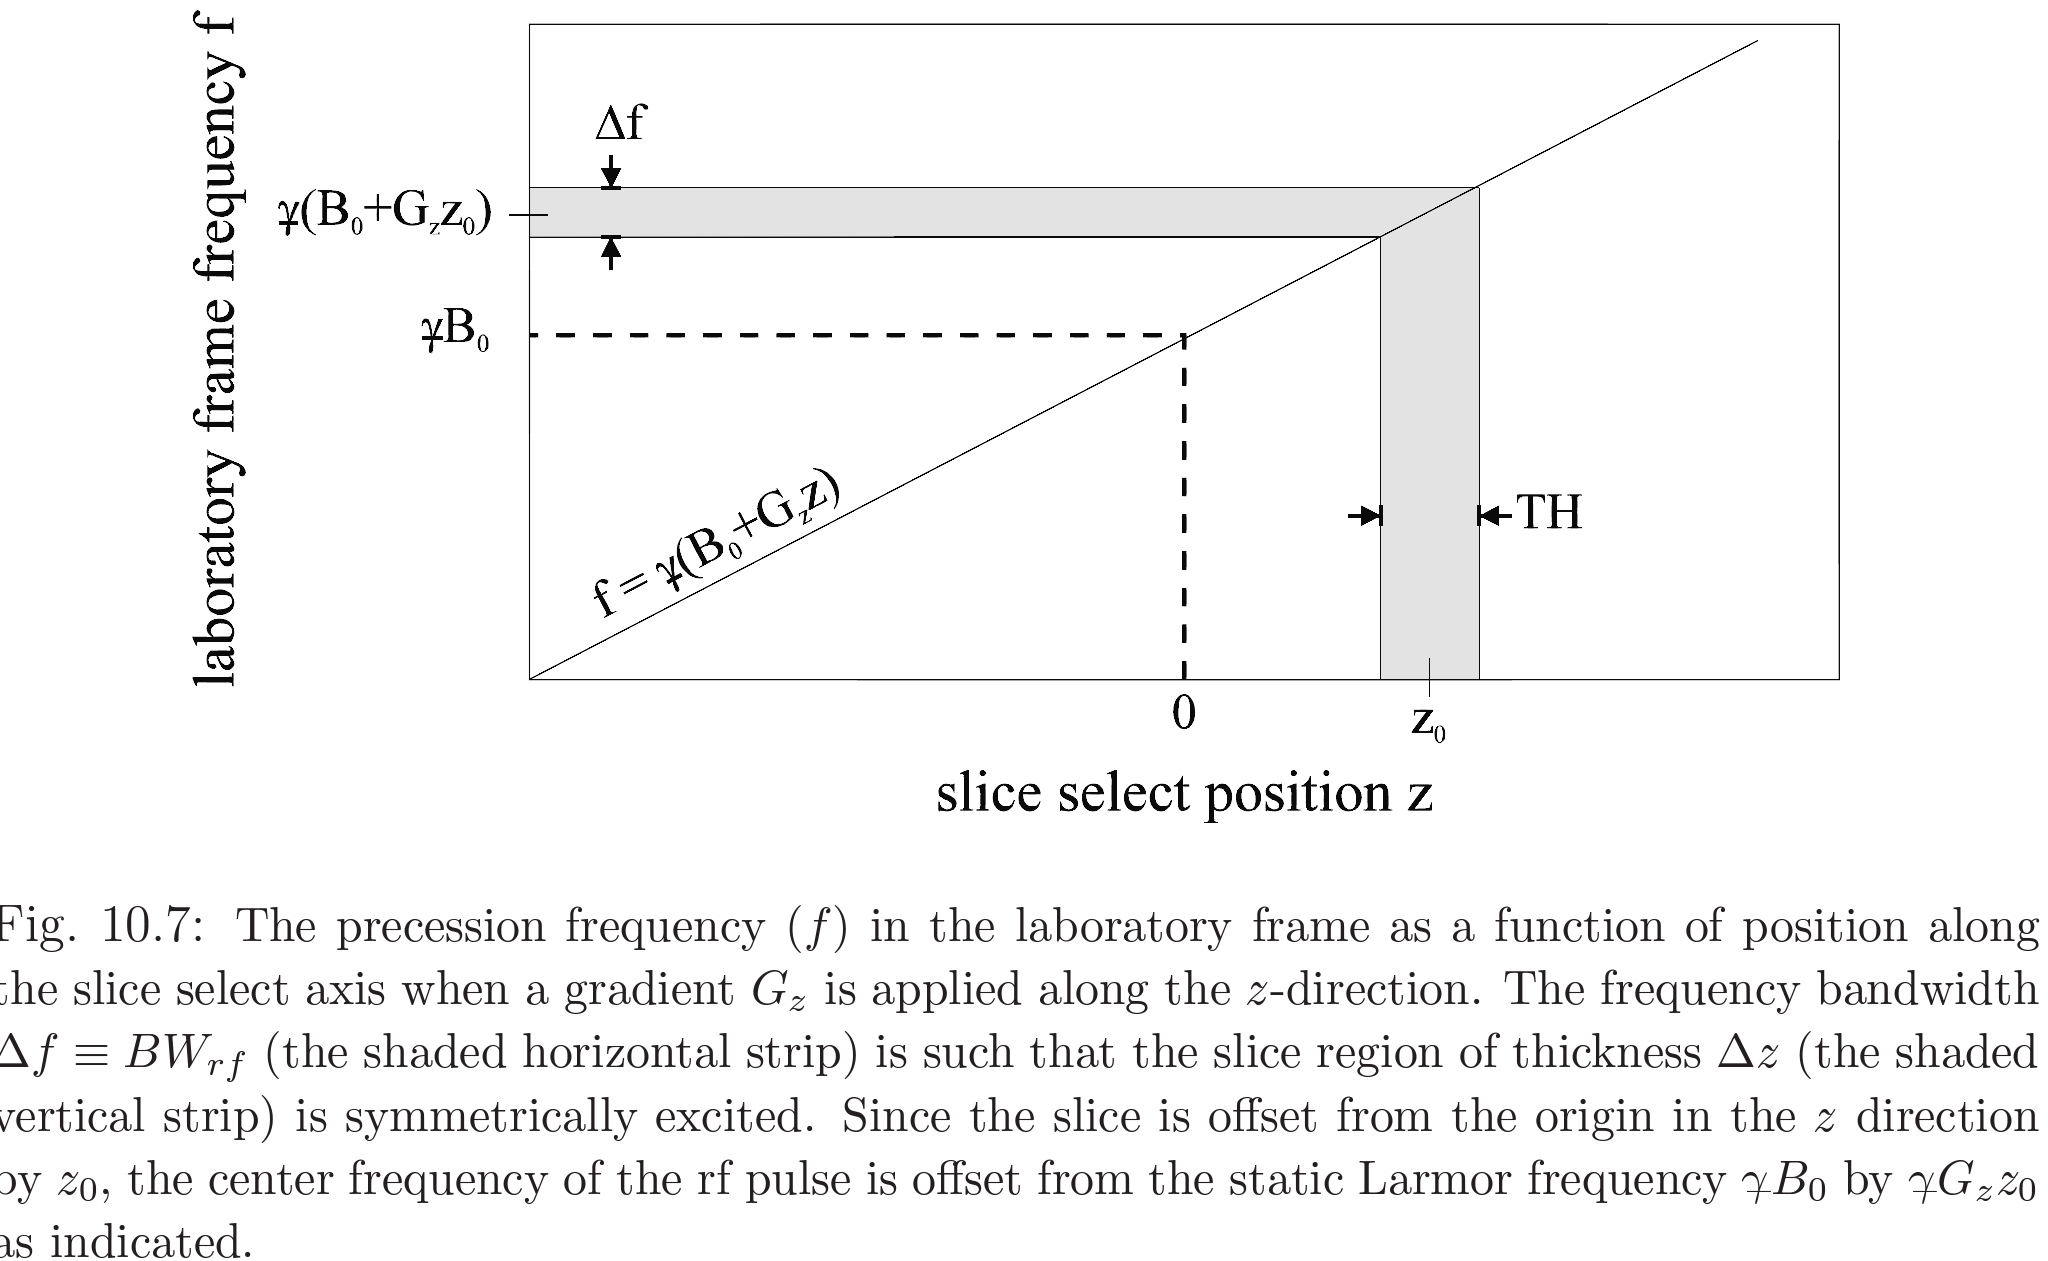
\includegraphics[trim={0cm 0cm 0 0},clip, keepaspectratio,width=0.4\textwidth]{sliceGBW}\label{fig:sliceGBW}\end{figure}
\end{frame}

\begin{frame}[allowframebreaks]{Nyquist criterion, resolution and contrast}

\begin{align*}
&(FOV)^{-1}\Delta k<\frac{1}{A}\\
&(\Delta k_R=\gammabar\int_t^{t+\Delta t}d t'G_R(t')=\frac{1}{L_R}<\frac{1}{A_R})\\
&f_R=BW_{read}=\frac{1}{\Delta t}=\gammabar G_RL_R>\gammabar G_RA_R
\end{align*}
Risoluzione: $\Delta x=\frac{1}{2n\Delta k}$, $k=(-n\Delta k,(n-1)\Delta k)$.

\begin{align*}
&\SNR/Vxl\propto\frac{\sqrt{N_{aqr}}}{\sigma_0}\quad \Delta t= \frac{1}{\BW_{read}},\ T_s=N_x\Delta t\\
&\SNR/Vxl\propto \frac{\Delta x\Delta y\Delta z\sqrt{N_a}}{\BW_{read}/(N_xN_yN_z)}
\end{align*}
Degrading resolution to improve SNR.

\begin{align*}
&C_{AB}=S_A-S_B\\
&=\rho_{0A}(1-\exp{-\frac{T_R}{T_{1A}}})\exp{-\frac{T_E}{T*_{2A}}}-\rho_{0B}(1-\exp{-\frac{T_R}{T_{1B}}})\exp{-\frac{T_E}{T*_{2B}}}
\end{align*}
Weighting
\end{frame}

\part{Interazione momenti magnetici campi magnetici esterni: equazioni di Bloch}\linkdest{MagneticR}
\section{Momenti magnetici elementari e magnetizzazione della materia: interazione con campo statico.}\linkdest{magnetizzation}

\begin{frame}{Signal from magnetized material}
%succo
\begin{align*}
&emf=-\TDof{t}\int d^3r\vec{M}(\vec{r},t)\cdot\vec{\mathcal{B}}_{rec}\\
&S\propto \frac{\gamma^3B_0^2\rho_0}{T}
\end{align*}
\end{frame}
%
\begin{wordonframe}{Magnetizzazione longitudinale all'equilibrio}
La magnetizzazione longitudinale di equilibrio \'e determinata dalla probabilit\'a di occupazione livello energetico $\exp{\exp{-\frac{\scap{m}{B}_0}{KT}}}\approx1-\frac{\scap{m}{B}_0}{KT}$: l'''eccesso'' di spin con con campo $B_0$ \'e $N\frac{\hbar\omega_0}{2KT}$. $\mu=\gamma\vec{J}$, $\gamma=\SI{1.67e8}{\rad\per\tesla\per\second}$ ([\si{\newton\meter\per\tesla}], [\si{\ampere\square\meter}]).
La magnetizzazione risultante \'e $M_0=\rho_0\frac{\gamma^2\hbar^2}{4KT}B_0$. (momento dipolo magnetico per unit\'a di volume)
\end{wordonframe}

\begin{frame}[allowframebreaks]{Equazione del moto dipolo magnetico}
\begin{columns}[T]\begin{column}{0.5\textheight}
\begin{block}{Equazione del moto (bloch0)}
\begin{align*}
&\TDy{t}{\vec{\mu}}=\gamma\vec{\mu}\wedge\vec{B}\\
&|d \mu|=\mu\sin{\theta}d \phi=\gamma\mu B\sin{\theta} dt\\
&\TDof{t}\vec{\mu}^2=0,\ \TDof{t}(\scap{\mu}{B}_0)
\end{align*}
\end{block}
%%succo
\begin{block}{Soluzioni campo B costante: precessione }
\begin{align*}
&\omega=|\TDy{t}{\phi}|=\gamma B\\
&\Rightarrow\ \phi=-\omega_0+\phi_0\\
&\mu_+(t)=\mu_x(t)+i\mu_y(t)\\
&=|\mu_+(t)|\exp{i\phi(t)}
\end{align*}
\end{block}

\end{column}\begin{column}{0.5\textheight}
\begin{block}{Momento magnetico nucleare}
\begin{columns}  \begin{column}{0.05\textwidth}\Pproton\end{column} \begin{column}{0.95\textwidth}
Rapporto giromagnetico: $\vec{\mu}=\gamma\vec{J}$, $\gamma=\SI{2.675e8}{\rad\per\second\per\tesla}$, $\gammabar=\SI{42.58}{\mega\hertz\per\tesla}$.
\end{column}  \end{columns}
\begin{align*}
&\mu_B=\frac{e\hbar}{2m_e}=\SI{9.27e-24}{\ampere\per\square\meter}\\
&\mu_B=\frac{e\hbar}{2m_n}=\SI{5.05e-27}{\ampere\per\square\meter}
\end{align*}
\end{block}
\begin{block}{Momento delle forze}
\begin{align*}
&(\vec{F}=\TDy{t}{\vec{p}})\ d \vec{F}=\vecp{J}{B}\\
&(=Id \vec{l}\wedge\vec{B})\\
&d\vec{N}=\vec{r}\wedge d \vec{F}=\vec{x}\wedge(\vecp{J}{B})
\end{align*}
\end{block}
\end{column}  \end{columns}
\end{frame}

\begin{wordonframe}{spin e dipoli magnetici}

\begin{columns}\begin{column}{0.5\textwidth}
\begin{figure}[!ht]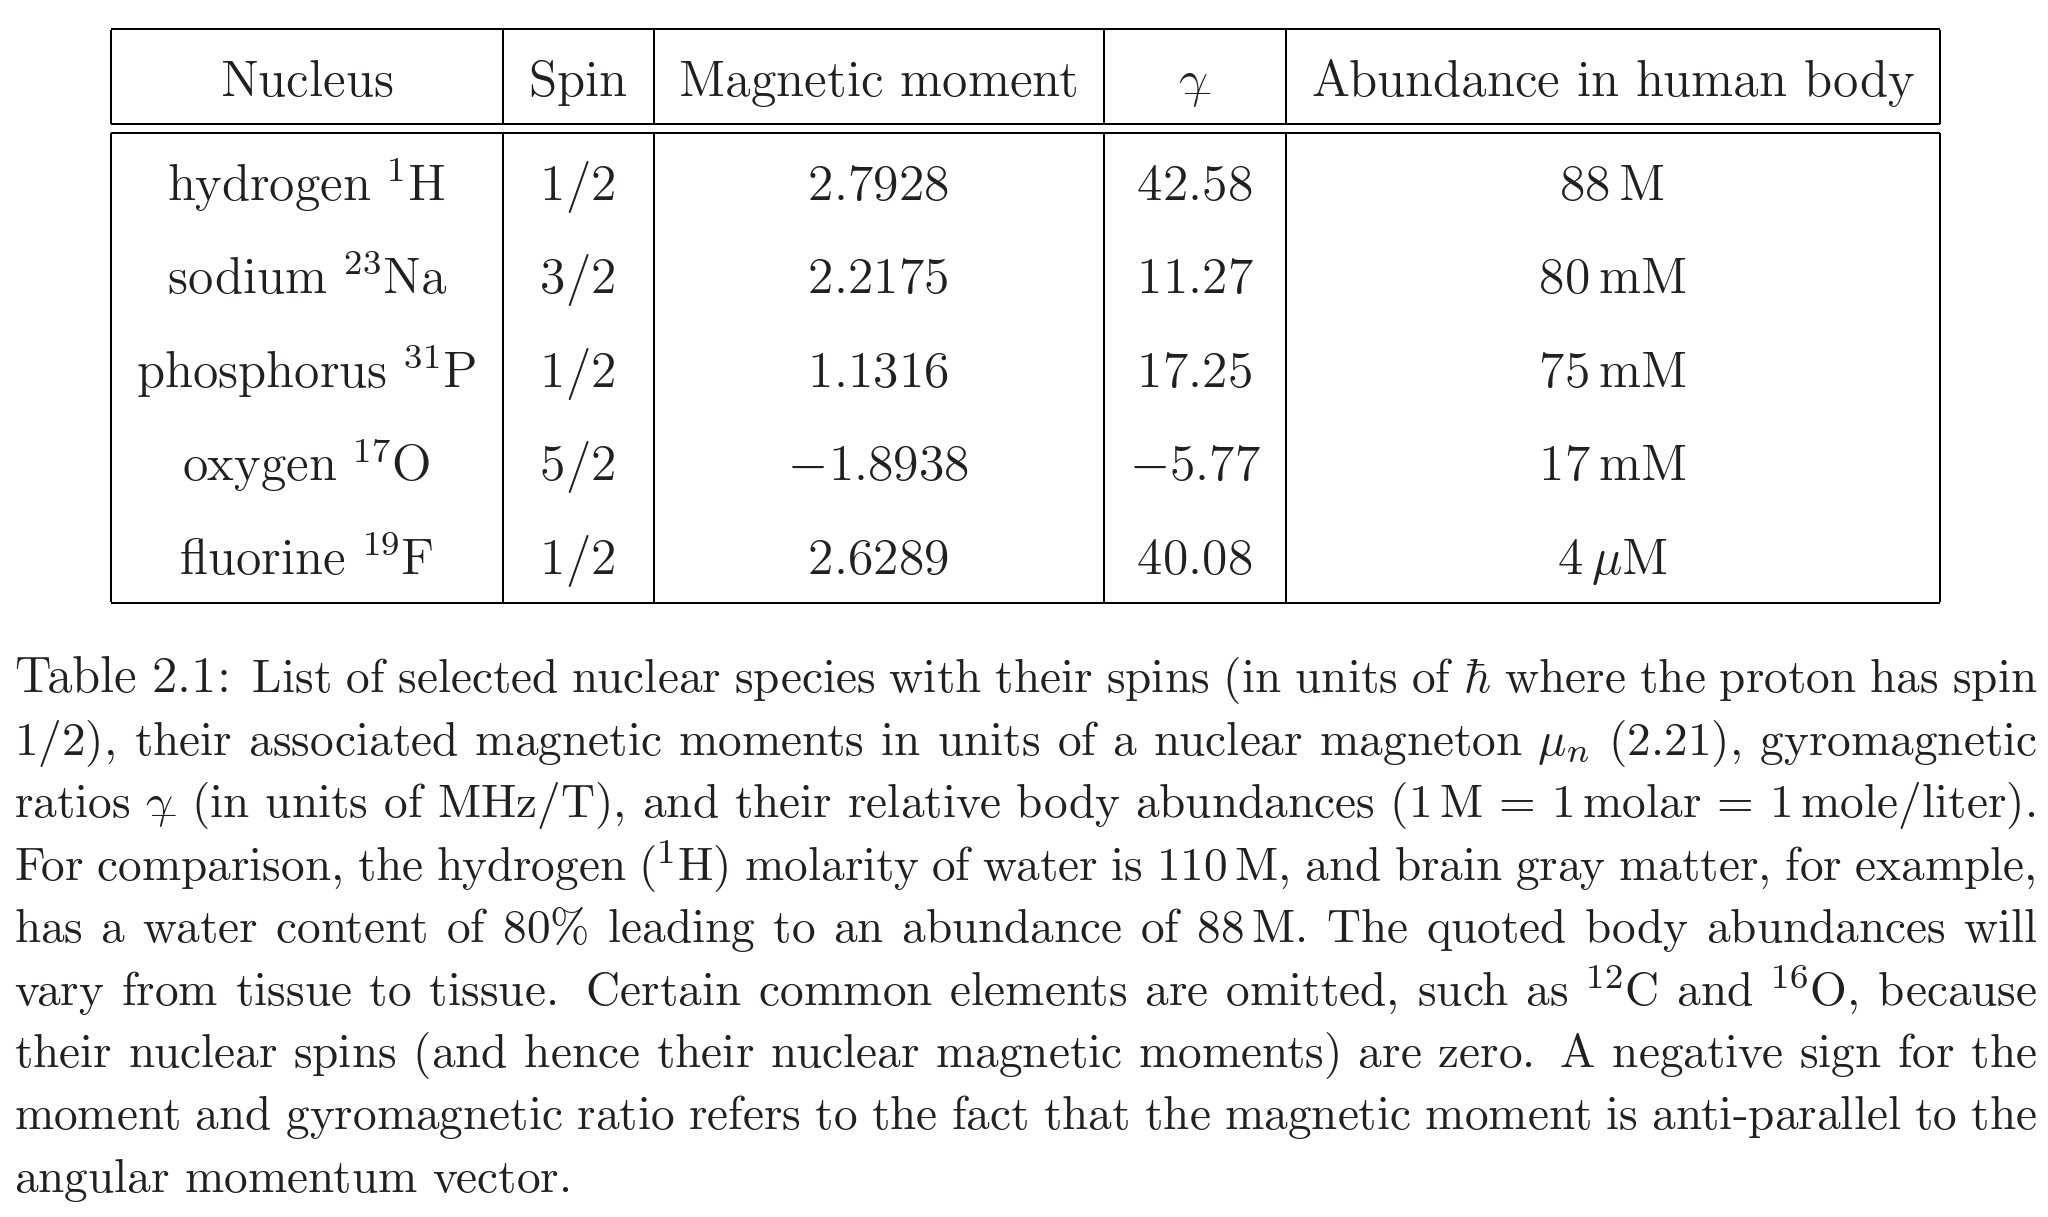
\includegraphics[trim={0cm 0cm 0 0},clip, keepaspectratio,width=0.99\textwidth]{nuclei}\label{fig:nuclei}\end{figure}
\end{column} \begin{column}{0.5\textwidth}
\begin{align*}
&\gamma=\frac{\mu}{J}\\
&\frac{\gamma_n}{2\pi g_n}=\frac{\mu_N}{h}=\SI{7.6}{\mega\hertz\per\tesla}\\
&\gamma_e=-2 \frac{e}{2m_e}\\
&\gamma_p=2.79\frac{e}{2m_p}\\
&\gamma_n=-1.91\frac{e}{2m_n}
\end{align*}
\end{column}\end{columns}
\begin{columns}  \begin{column}{0.5\textwidth}
Atomo con Z elettroni
\begin{align*}
&\vec{\mu}=-g_J \frac{e}{2m}\vec{J}\\
&g_J=\frac{3}{2}+\frac{S(S+1)-L(L+1)}{J(J+1)}
\end{align*}

\end{column} \begin{column}{0.5\textwidth}
Frequenze di Larmor: moto orbitale elettroni $\nu_L=\SI{1.4e10}{\hertz\per\tesla}$, spin elettronico $\nu_L=\SI{2.8}{\mega\hertz\per\gauss}$, spin protonico $\nu_L=\SI{4.3}{\kilo\hertz\per\gauss}$
\end{column}  \end{columns}
\end{wordonframe}

\section{Condizione di risonanza: campo trasverso $B_1$}\linkdest{resonance}

\begin{frame}[allowframebreaks]{Campo a radiofrequenza rotante}
\begin{block}{SR rotante}
\begin{align*}
&\TDy{t}{\vec{\mu}}=(\TDy{t}{\vec{\mu}})'+\vecp{\Omega}{\mu}=\gamma\vecp{\mu}{B}\\
&(\TDy{t}{\vec{\mu}})'=\gamma\vec{\mu}\wedge\vec{B}_{eff}\quad B_{eff}=\vec{B}+\frac{\vec{\Omega}}{\gamma}
\end{align*}
\end{block}
\begin{block}{EOM per campo $B_1$ a RF circolare}
\begin{equation*}
\vec{B}_1^{circ}=B_1(\hat{x}\cos{(\omega t)}-\hat{y}\sin{(\omega t)})
\end{equation*}
fermo nel riferimento rotante: $\vec{\Omega}=-\omega\hat{z}$.
\begin{align*}
&(\TDy{t}{\vec{\mu}})'=\vec{\mu}\wedge[\hat{z}'(\omega_0-\omega)+\hat{x}'\omega_1]=\gamma\vec{\mu}\wedge\vec{B}_{eff}\\
&\omega_0=\gamma B_0,\ \omega=\text{RF lab freq.},\ \omega_1=\gamma B_1
\end{align*}
\end{block}
\begin{block}{on-resonance condition}
\begin{columns}[T]
    \begin{column}{0.5\textheight}
 %%succo
    Per $\omega=\omega_0$:
\begin{align*}
&(\TDy{t}{\vec{\mu}})'=\omega_1\vec{\mu}\wedge\hat{x}'
\end{align*}
Flip-angle: $\Delta\theta=\gamma B_1\tau$.
    \end{column}
    \begin{column}{0.5\textheight}
    RF on-resonance solution
    \begin{align*}
    &\vec{\mu}(t)=R_{x'}(\phi_1(t))\vec{\mu}(0)\\
    &\phi_1(t)=\omega_1t\to\int_{t_0}^td t'\omega_1(t')
    \end{align*}
    \end{column}
\end{columns}
\end{block}
\end{frame}

\begin{wordonframe}{SR rotanti e on-resonance condition (chap 3)}
\begin{equation*}
\TDy{t}{\vec{V}}=(\TDy{t}{V})'+\vecp{\Omega}{V}
\end{equation*}
\begin{block}{Problema 3.3}

\end{block}
\end{wordonframe}

\section{Evoluzione componenti magnetizzazione longitudinale e trasversa: precessione + spin-lattice + spin-spin.}\linkdest{blocheq}

\begin{frame}[allowframebreaks]{Magnetizzazione in campo esterno: $T_1$, $T_2$. Equazione di Bloch.}
\begin{columns}[T]
\begin{column}{0.45\textheight}
\begin{block}{Magnetizzazione}
($M=\frac{1}{2}\vecp{x}{J}$)
Momento di dipolo magnetico per unit\'a di volume:
\begin{equation*}
\vec{M}=\frac{1}{V}\sum\vec{\mu}_i
\end{equation*}
V=voxel: volume dove campo magnetico omogeneo, spin hanno stessa fase.
\end{block}
\begin{block}{Dephasing due to $B_{ext}$ inhomogeneities. Spin ECHO}
%succo
$\frac{1}{T_2*}=\frac{1}{T_2}+\frac{1}{T_2}$: se domina $T_2'$ dovuto a disomogeneit\'a compo magnetico esterno $\magort{}$ pu\'o essere rifasata.
\end{block}
\end{column}
\begin{column}{0.55\textheight}
\begin{block}{Interazioni spin-lattice: $T_1$.}
%succo
\begin{align*}
&\TDy{t}{M_z}=\frac{(M_0-M_z)}{T_1}\\
&M_z(t)=M_z(0)\exp{-\frac{t}{T_1}}+M_0(1-\exp{-\frac{t}{T_1}})
\end{align*}
\end{block}
\begin{block}{Local field variation: dephasing. $T_2$}
\begin{align*}
&\TDy{t}{\magort}=(\gamma\magort{}\wedge\vec{B}_{ext})_{NR}-\frac{1}{T_2}\magort{}\\
&\magort{}(t)=\magort{}(0)\exp{-\frac{t}{T_2}}
\end{align*}
\end{block}

\begin{block}{Short/long lived pulses.}
$\Delta\omega\tau_{RF}\geq\frac{1}{4\pi}$. Short: $\Delta\omega_1\gg(\frac{1}{T_1},\frac{1}{T_2})$, ignore decay during pulse. Long: steady state.
\end{block}
\end{column}
\end{columns}
\clearpage Lorentzian shape Mz as fuction of $\omega$: lezione 1 esr
\end{frame}

\begin{wordonframe}{Rilassamento spin-lattice, spin-spin e inomogeneit\'a del campo (chap 4)}
\begin{block}{Densit\'a di energia potenziale magnetica}
Gli spin tendono ad allinearsi col campo magnetico per minimizzare la densit\'a d'energia potenziale, $U_M=-\scap{M}{B}=M_zB_0$: si hanno interazioni spin lattice.
\end{block}
Legge di Curie: $M_0=C\frac{B_0}{T}$,valore di equilibrio.
\begin{block}{Evoluzione $M_z$, inizio arbitrario}
\begin{align*}
&M_z(t)=M_z(0)\exp{-\frac{t}{T_1}}+M_0(1-\exp{-\frac{t}{T_1}})\\
&0\to t_0,\ t\to t-t_0
\end{align*}
\end{block}
\end{wordonframe}

\begin{frame}{Equazione di Bloch}
%succo
    \begin{equation*}
        \TDy{t}{\vec{M}}=\gamma\vec{M}\wedge\vec{B}_{ext}+\frac{1}{T_1}(M_0-M_z)\hat{z}-\frac{1}{T_2}\magort{}
    \end{equation*}
    soluzioni:
    \begin{align*}
&M_x(t)=\exp{-\frac{t}{T_2}}(M_x(0)\sin{(\omega_0t)}+M_y(0)\cos{(\omega_0t)})\\
&M_y(t)=\exp{-\frac{t}{T_2}}(M_y(0)\cos{(\omega_0t)}-M_x(0)\sin{(\omega_0 t)})\\
&M_z(t)=M_z(0)\exp{-\frac{t}{T_1}}+M_0(1-\exp{-\frac{t}{T_1}})\\
&M_+(t)=\exp{-i\omega_0t-t/T_2}M_+(0)\to|M_+(t)|\exp{i\phi(t)}
    \end{align*}
    Per $\vec{B}_{ext}=B_0\hat{z}+B_1\hat{x}$, le equazioni di Bloch sono, con $\Delta\omega=\omega_0-\omega$:
    \begin{align*}
&(\dot{M}_{z'})'=-\omega_1M{y'}+\frac{M_0-M_z}{T_1}\\
&(\dot{M}_{x'})'=\Delta\omega M_{y'}-\frac{M_{x'}}{T_2}\\
&(\dot{M}_{y'})'=-\Delta\omega M_{x'}+\omega_1M_z-\frac{\omega M_{y'}}{T_2}
    \end{align*}
\end{frame}

\begin{wordonframe}{Regimi di applicazione}
\begin{itemize}
    \item $|H_1|\ll|H_0|$
    \item Ehrenfest adiabaticity: $\vec{H}$ and $\vec{M}$ formano angolo costante: How slowly we must change $\vec{H}$ direction so that $\vec{M}$ preserve its angle (preserving its interaction energy)? If $\vec{\Omega}$ is the rotation of $\vec{H}$ in rotating frame with $\vec{H}$
    \begin{equation*}
        (d/dt)'\vec{M}=(\gamma\vec{H}-\Omega)\wedge\vec{M}
    \end{equation*}
    quindi $\Omega\ll\gamma\vec{H}$
    \item Adiabaticity in rotating frame. We take for $\vec{H}=\hat{x}H_1\cos{\omega t}+\hat{y}H_1\sin{\omega t}+\hat{z}H_0$ Adiabatic passage through resonance $\omega=\omega_0=\gamma H_0$ (slowly sweep of $\omega$ through $\omega_0=\gamma H_0$). Defining effective field $\vec{H}_e=\vec{H}-\vec{\omega}/\gamma$. $\vec{M}=\vec{M}_0=\chi_0\vec{H}_0$ pointing along $\vec{H}_0$ and approx along $\vec{H}_e$ ($H_1\ll H_0$, $\omega\ll\gamma H_0$): initial motion is a precession of $\vec{M}$ around $\vec{H}_e$ viewed from rotating frame.
    How slowly we must change $\vec{H}_e$ in order $\vec{M}$ to follow?
    Magnetic field turn impercettible during period of Larmor precession about it:
    \begin{equation*}
    \invers{H}_1|(d/dt)(\vec{H}_0-\vec{\omega}/\gamma)|\ll\gamma H_1
    \end{equation*}
    \item rapid passage. Slowest precession in rotating frame when $\gamma\vec{H}_e=\gamma\vec{H}_1$: se $1/T_1$ or $1/T_2$ exceed $\gamma H_1$ relaxation processes cause $\vec{M}$ to decay, $1/T_2\ll\gamma H_1$. ($1/T_1\leq1/T_2$)
    \item Slow passage. Steady state condition $\TDy{t}{M_z}=0$
    \end{itemize}
\end{wordonframe}

\begin{frame}{Soluzione equazioni di Bloch: condizioni stazionarie}
    \begin{columns}[T]
    \begin{column}{0.5\textwidth}
    \begin{align*}
    &\PDy{t}{M_x}=\PDy{t}{u}=0=\frac{-u}{T_2}+v\Delta\omega\\
    &\PDy{t}{M_y}=\PDy{t}{v}=0=\frac{-v}{T_2}-u\Delta\omega-\omega_1M_z\\
    &\PDy{t}{M_z}=0=\omega_1v+\frac{M_z-M_0}{T_1}\\
    \end{align*}
    con $\Delta\omega=\omega-\omega_0$. Soluzioni:
    \begin{align*}
    &u=M_0\frac{\omega_1\Delta\omega T_2^2}{1+(T_2\Delta\omega)^2+\omega_1^2T_1T_2}\\
    &u=M_0\frac{\omega_1T_2}{1+(T_2\Delta\omega)^2+\omega_1^2T_1T_2}\\
    &M_z=M_0\frac{1+(T_2\Delta\omega)^2}{1+(T_2\Delta\omega)^2+\omega_1^2T_1T_2}\\
    \end{align*}
    \end{column}
    \begin{column}{0.5\textwidth}
    \begin{figure}
        \centering
        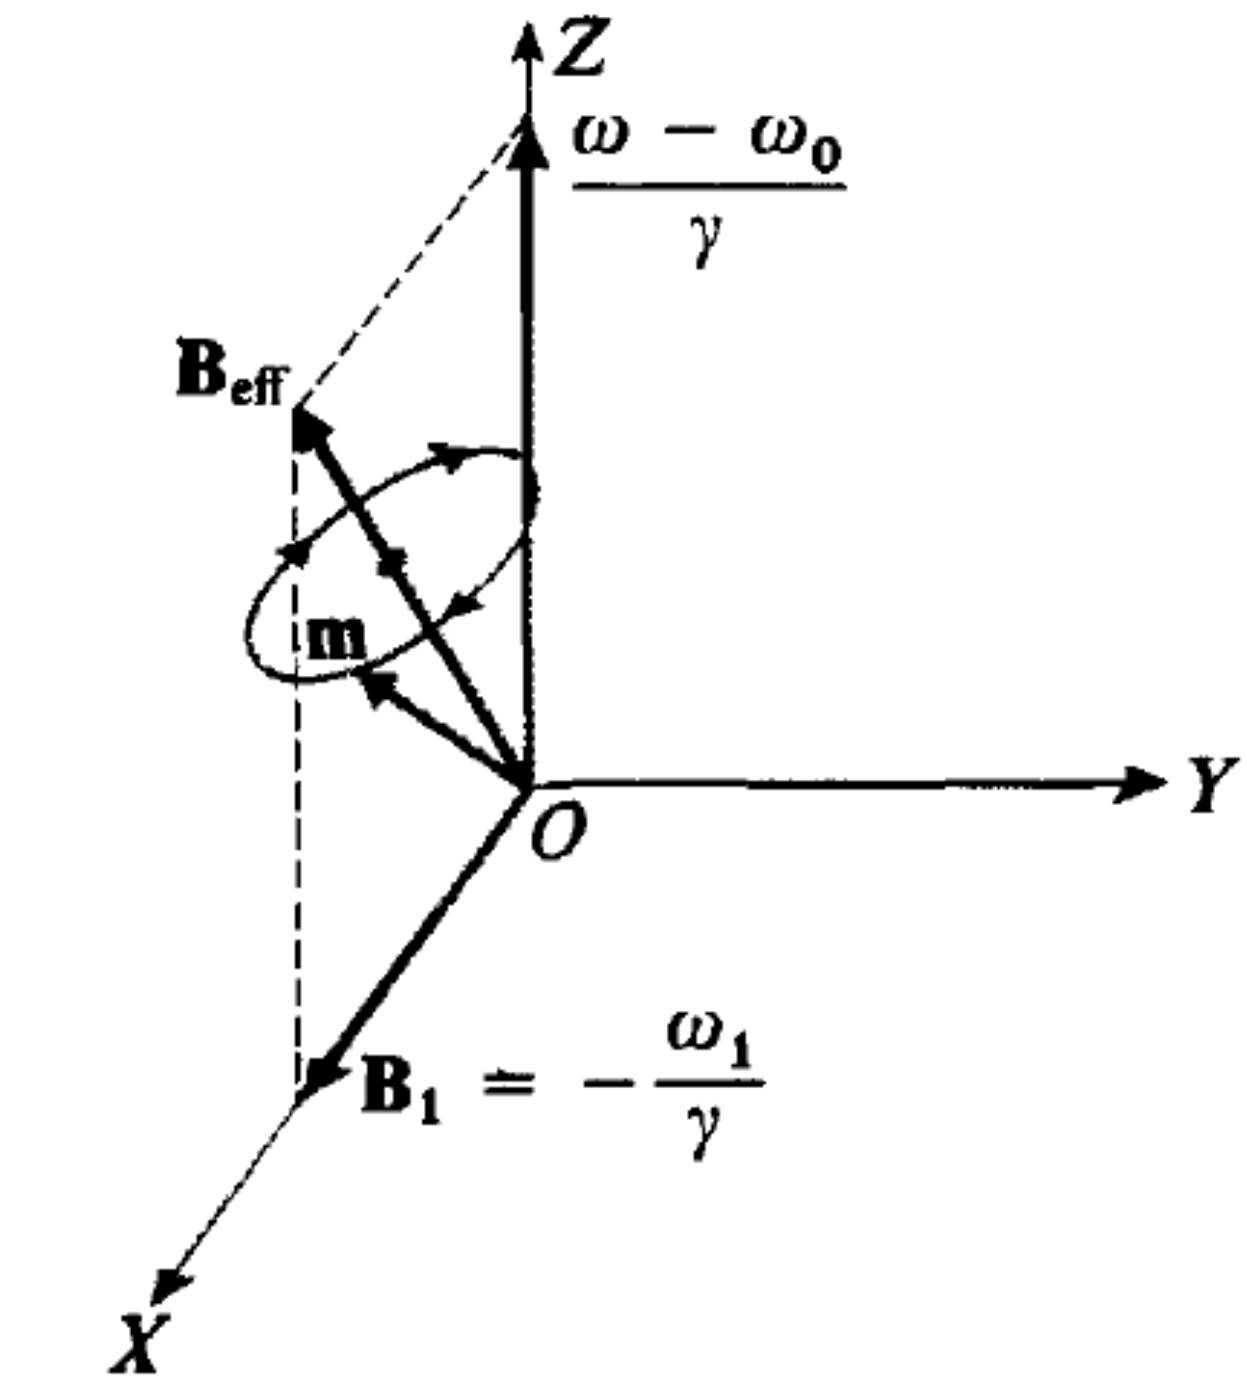
\includegraphics{MBrotCW}
        \label{fig:MBrotCW}
    \end{figure}
    Nel riferimento del Lab la magnetizzazione ruota con velocit\'a angolare costante:
    \begin{align*}
    &M_x=u\cos{\omega t}-v\sin{\omega t}=\sqrt{u^2+v^2}\cos{\omega t-\phi}\\
    &M_y=u\cos{\omega t}+v\sin{\omega t}=\sqrt{u^2+v^2}\sin{\omega t-\phi}\\
    &M_z=M_z
    \end{align*}
    Effetti del campo rotante
    \begin{itemize}
        \item Diminuzione componente $M_z$
        \item Magnetizzazione trasversa rotante con $B_1$ con ritardo $\phi$ rispetto a $B_1$: Il campo rotante compie lavoro positivo e l'energia corrispondente \'e assorbita dal mezzo.
    \end{itemize}
    \end{column}
    \end{columns}
\end{frame}

\begin{frame}{Importanza }
    
\end{frame}

\section{Tipi di rilassamento}

\begin{frame}{Sistema spin isolati (only intra group interaction??). Magnetizzazione, popolazione livelli e coerenza}
\begin{columns}[T]
\begin{column}{0.5\textwidth}
\begin{itemize}
\item RF: Coherence excitation ($\pi/2|_x$, $\pi|_x$ inversion of population.
\item $B_0$: Different population of Zeeman splitted levels in thermal equilibrium.
\end{itemize}
\begin{block}{Coerenza e popolazione}
\begin{figure}
    \centering
    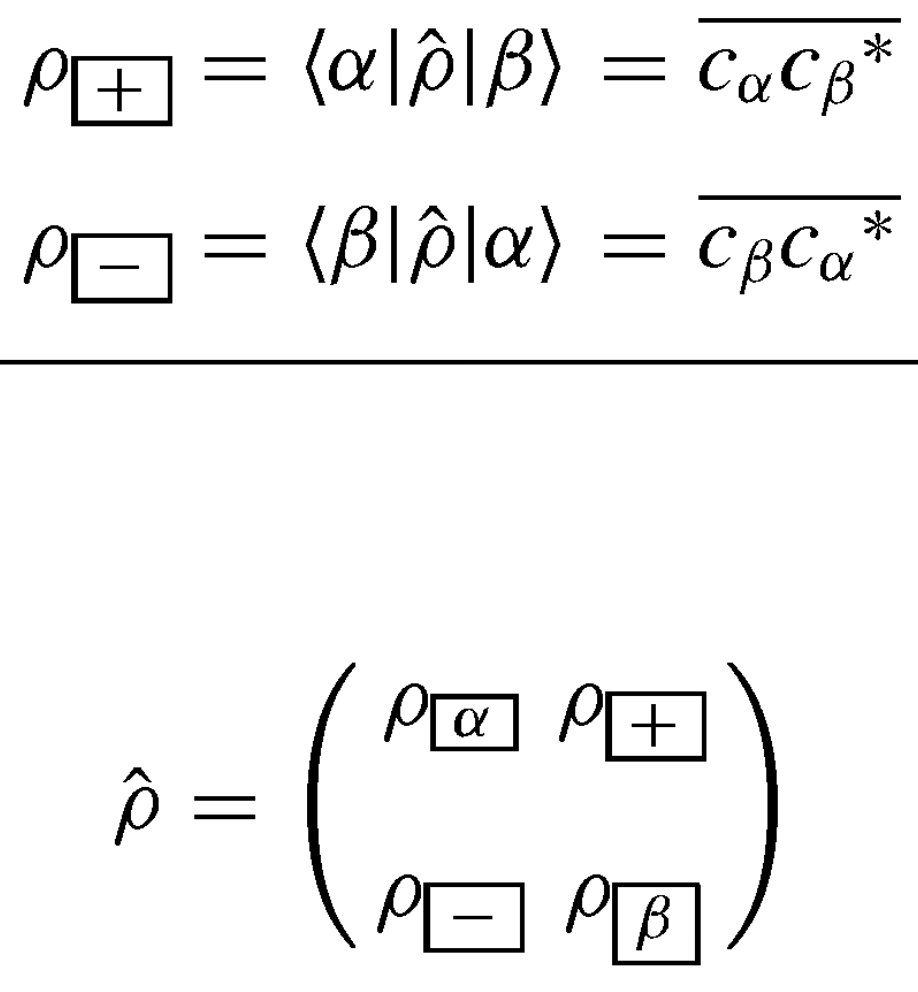
\includegraphics[height=0.4\textheight,keepaspectratio]{densitym}
    \label{fig:densitym}
\end{figure}
\begin{align*}
&M_z\propto\rho_{\alpha}-\rho_{\beta}\\
&M_x\propto\Re{\rho_-}, M_y\propto\Im{\rho_-}
\end{align*}

\end{block}
\end{column}
\begin{column}{0.5\textwidth}
\begin{block}{Spontaneous/induced emission in system of spin}
\begin{figure}[!ht]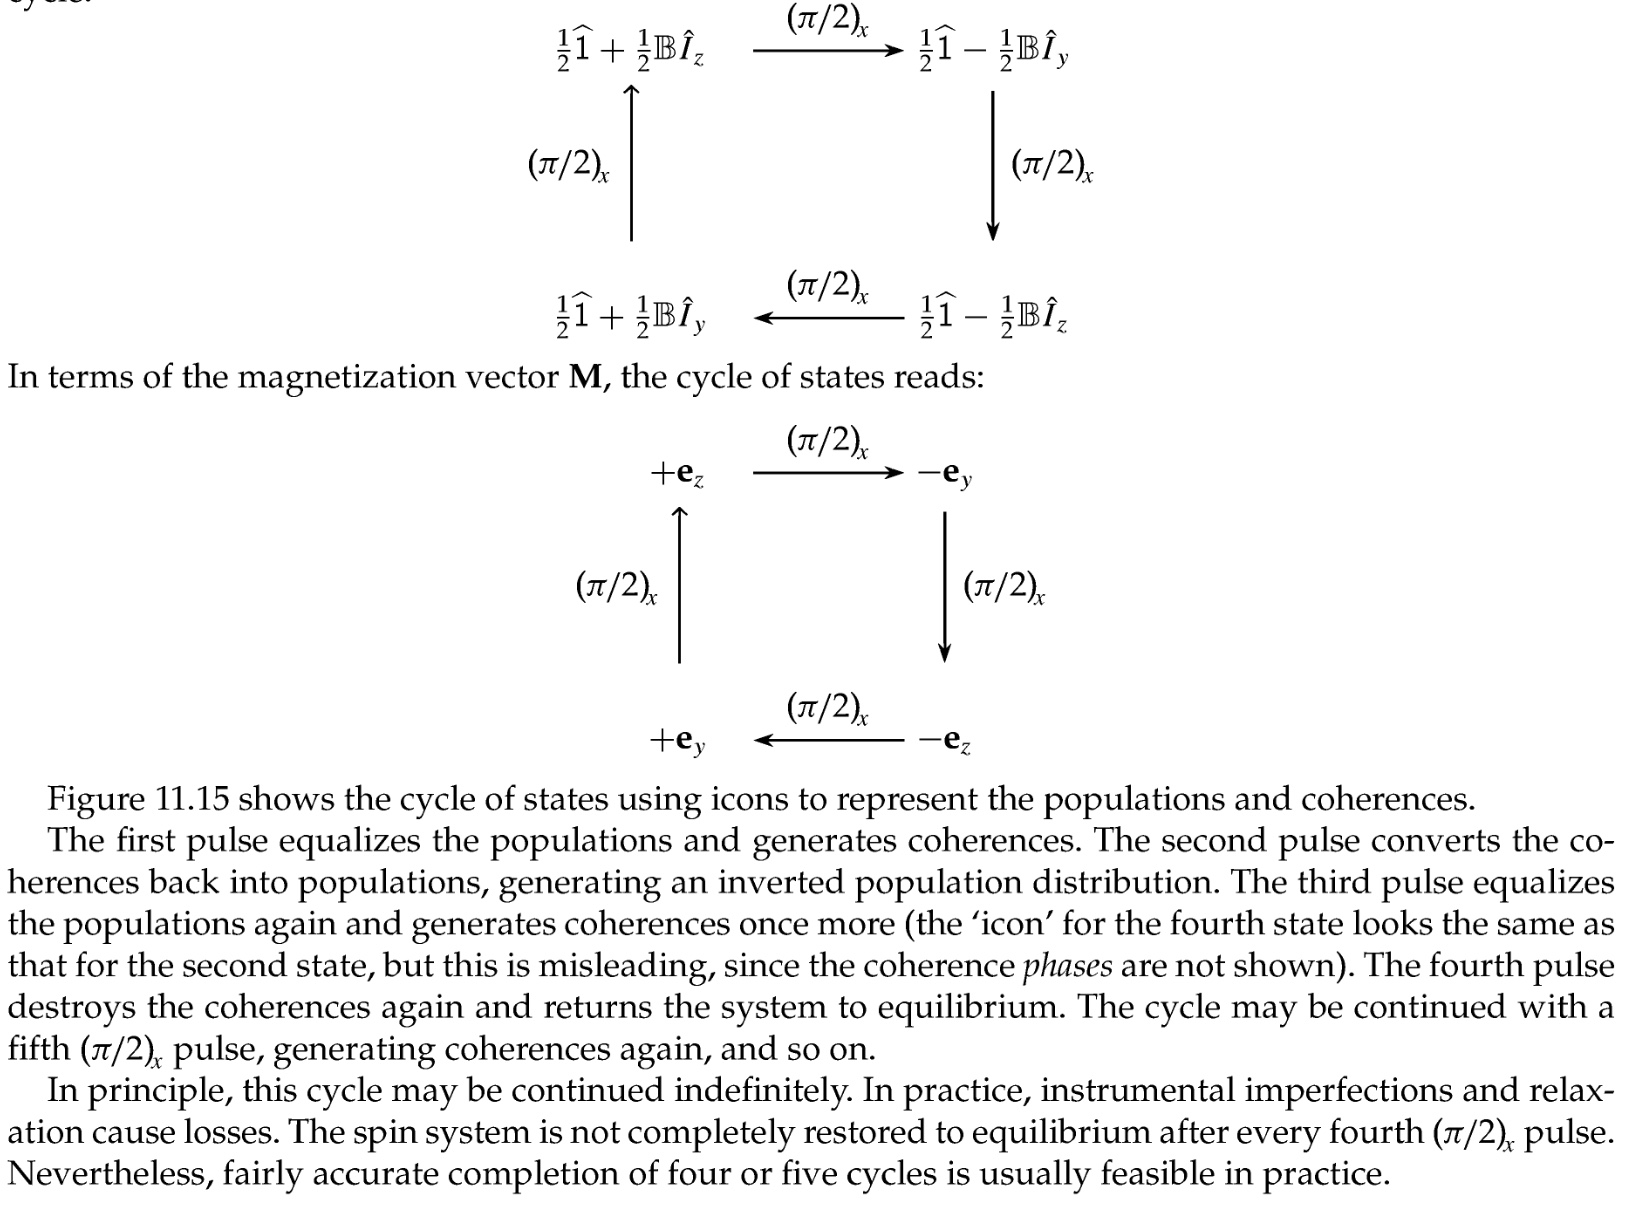
\includegraphics[trim={0cm 0cm 0 0},clip, keepaspectratio,width=0.9\textwidth]{RFcycle}\label{fig:RFcycle}\end{figure}
\end{block}
\end{column}
\end{columns}
\end{frame}

\begin{wordonframe}{Sistema di spin: Coerenza e popolazione}
L'energia del sistema viene aumentata dallo stato iniziale di equilibrio termico allo stato in cui le popolazioni sono in uguali, il secondo impulso aumenta ancora energia generando inversione della popolazione dei livelli mentre terzo e quarto fanno diminuire energia del sistema
\end{wordonframe}

\begin{frame}{Motional timescale. Averaging and relaxation}

    \begin{columns}[T]
    \begin{column}{0.5\textwidth}
    \begin{figure}
    \centering
    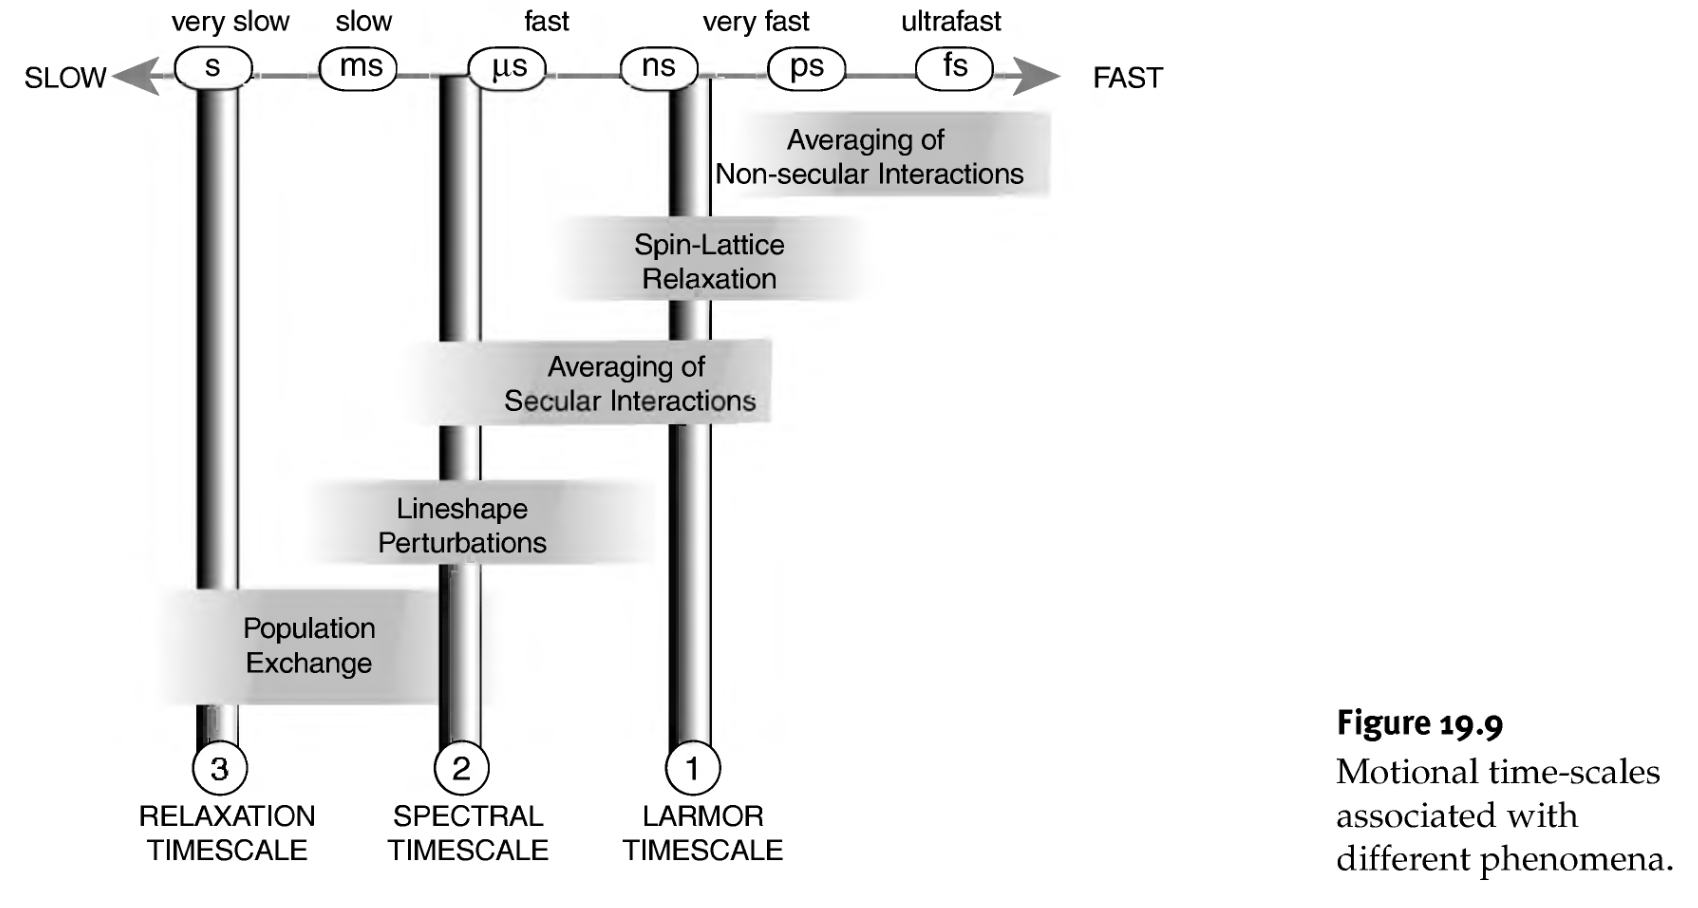
\includegraphics[width=0.99\textwidth, trim={0 0 15cm 0},clip]{motiontau}
    \label{fig:motiontau}
\end{figure}
    \end{column}
        \begin{column}{0.5\textwidth}
    \begin{figure}
    \centering
    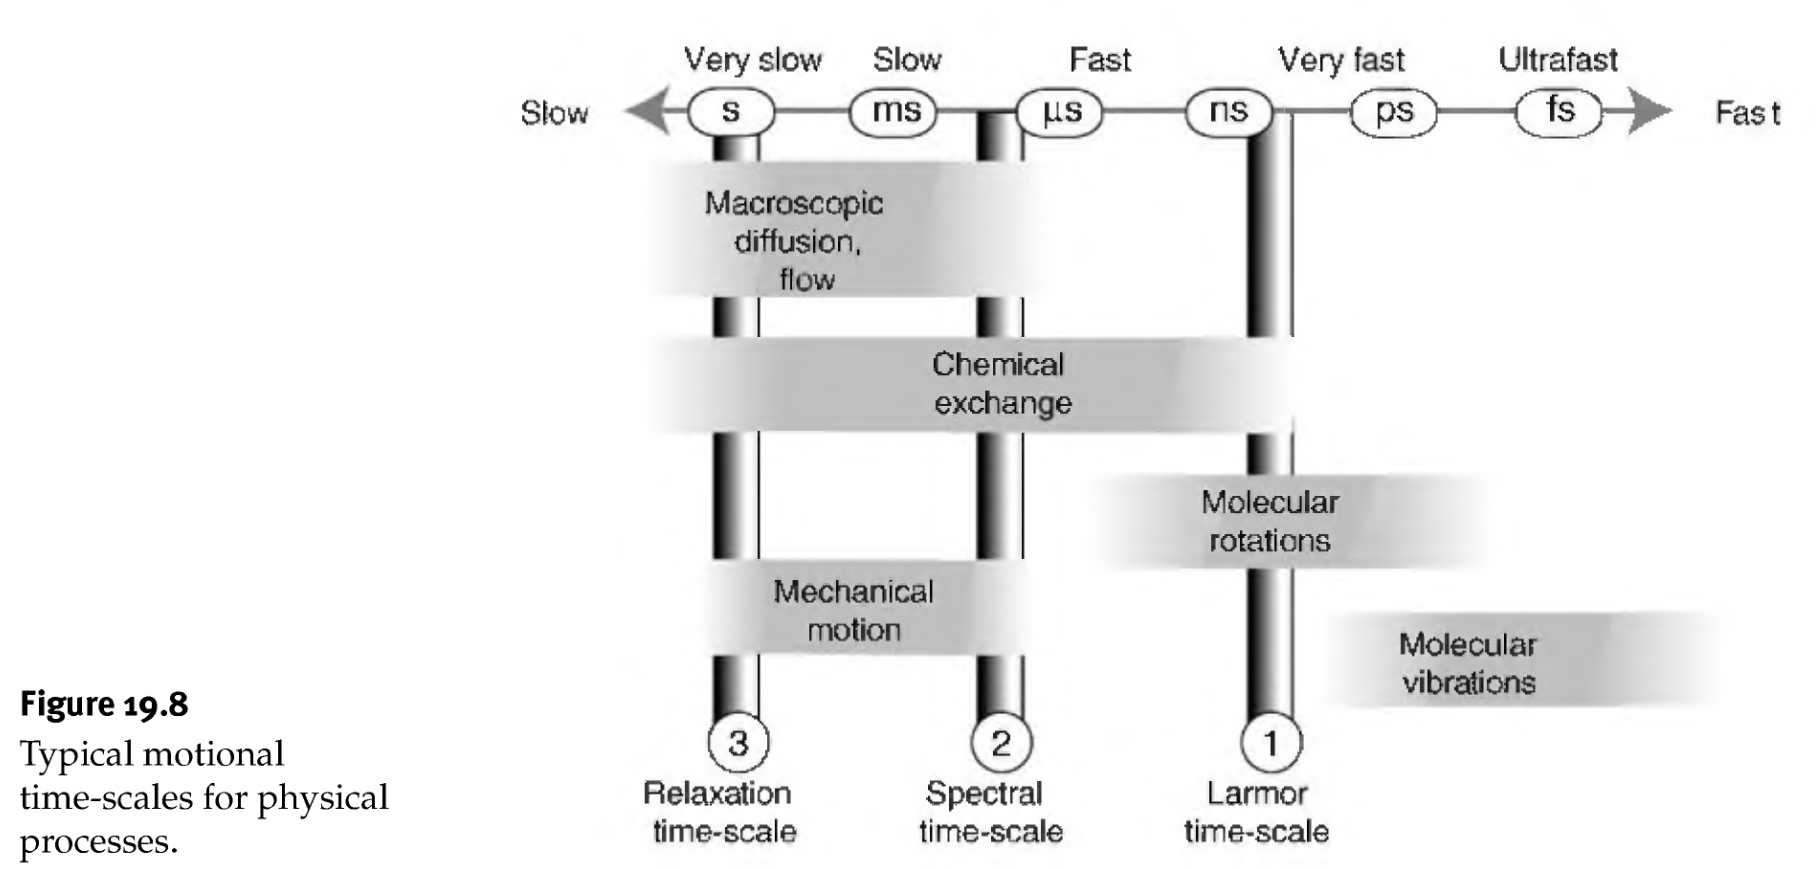
\includegraphics[width=0.99\textwidth, trim={15cm 0 1cm 0},clip]{tauproc}
    \label{fig:tauproc}
\end{figure}
    \end{column}
    \end{columns}
    \begin{itemize}
    \item Secular approximation arise because spin dynamics is dominated by interactions with large externalo magnetic field. Diagonal blocks.
    \item Motional averaging: can average over sufficient fast molecular motion
\end{itemize}
The discarded part are responsable for relaxation.
\end{frame}

\begin{frame}{Random field and spectral density}
\begin{columns}[T]
\begin{column}{0.5\textwidth}
\begin{block}{Autocorrelation function}
\begin{align*}
&\exv{B_x(t)}=0,\ \exv{B_x^2(t)}\neq0\\
&G(\tau)\exv{B_x(t)B_x(t+\tau)}\neq0
\end{align*}
\end{block}
\begin{block}{Densit\'a spettrale}
\begin{align*}
&J(\omega)=2\int_0^{+\infty}G(\tau)\exp{-i\omega\tau}d\,\tau\\
&\to2\exv{B_x^2}A(\omega;0,\invers{\tau_c})\\
&=2\exv{B_x^2}\frac{\tau_c}{1+\omega^2\tau_c^2}
\end{align*}
\end{block}
\end{column}
\begin{column}{0.5\textwidth}
Spin indipendent assumption: not strictly true for any mechanism
\begin{block}{Correlation time}
\begin{equation*}
G(\tau)=\exv{B_x^2}\exp{-\tau/\tau_c}
\end{equation*}
How long it take before random field changes sign
\end{block}
\end{column}
\end{columns}
\end{frame}

\begin{frame}{Transition probability and spin-lattice relaxation}
\begin{columns}[T]
\begin{column}{0.6\textwidth}
\begin{block}{Transition probability $\ket{\alpha}\to\ket{\beta}$ and thermal equilibrium}
\begin{align*}
&W_-=\invers{\tau}\exv{|\braket{\beta|\alpha'}|^2}\\
&W_+=\invers{\tau}\exv{|\braket{\alpha|\beta'}|^2}\\
&\rho_{\alpha}^{eq}W_-=\rho_{\beta}^{eq}W_+
\end{align*}
\end{block}
\end{column}
\begin{column}{0.4\textwidth}
\begin{figure}
    \centering
    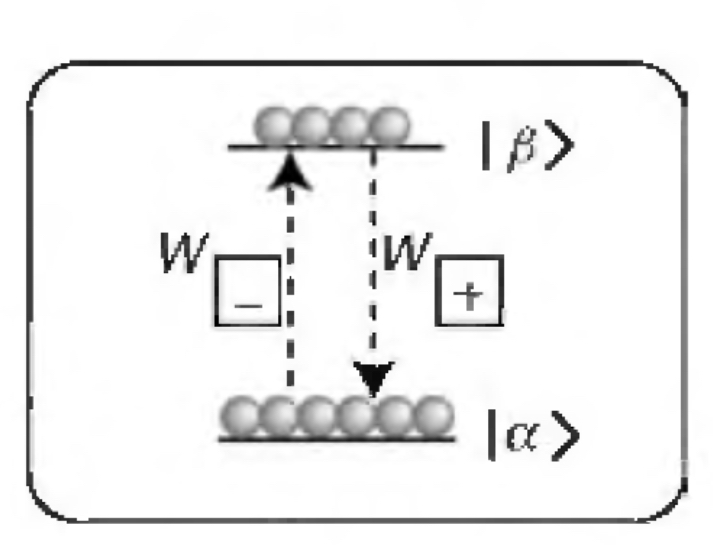
\includegraphics[keepaspectratio,width=0.9\textwidth]{transitionp}
    \label{fig:transitionp}
\end{figure}
\begin{align*}
&W_-=W(1-\frac{1}{2}\frac{\hbar\gamma B_0}{KT})\\
&W_+=W(1+\frac{1}{2}\frac{\hbar\gamma B_0}{KT})\\
&W=\frac{1}{2}\gamma^2\exv{B_x^2}\frac{\tau_c}{1+(\omega_0\tau_c)^2}
\end{align*}
\end{column}
\end{columns}
\begin{align*}
&\invers{T_1}=\gamma^2\exv{B_x^2}\frac{\tau_c}{1+(\omega_0\tau_c)^2}
\end{align*}
\end{frame}

\part{NMR imaging}\linkdest{NMRimaging}
\section{Impulsi e segnali}\linkdest{impulse}

\begin{frame}{Signal detection}
\begin{align*}
&emf=-\TDy{t}{\Phi_{coil}}=\TDof{t}\int\,d^3r\vec{M}(\vec{r},t)\cdot\vec{\mathcal{B}}_{rec}\\
&S\propto \frac{\gamma^3B_0^2\rho_0}{T}\\
&\mathcal{B}^{rec}=\frac{\vec{B}(\vec{r}')}{I}
\end{align*}
\end{frame}

\begin{frame}[allowframebreaks]{FID, Spin echo and $T_2$ measure}
\begin{block}{Free induction decay}%
$\pi/2$ pulse lungo $x'$:
\begin{align*}
&s(t)\propto\omega_0\int d^3r \exp{-\frac{t}{T_2(r)}}B_{\perp}(\vec{r})M_{\perp}(\vec{r},0)\exp{i[(\Omega-\omega(r))t+\phi_0(\vec{r})+\theta_B(\vec{r})]}\\
&\phi(\vec{r},t)=-\omega(r)t+\phi_0(\vec{r})=-\gamma B_z(\vec{r})t+\phi_0(\vec{r})
\end{align*}
Possibilit\'a che lòa frequenza di precessione cambi con la posizione $\omega(\vec{r})$
%B_x=B_{\perp}\cos{\theta_b}
\end{block}
\begin{block}{Repeated FID}
\begin{figure}[!ht]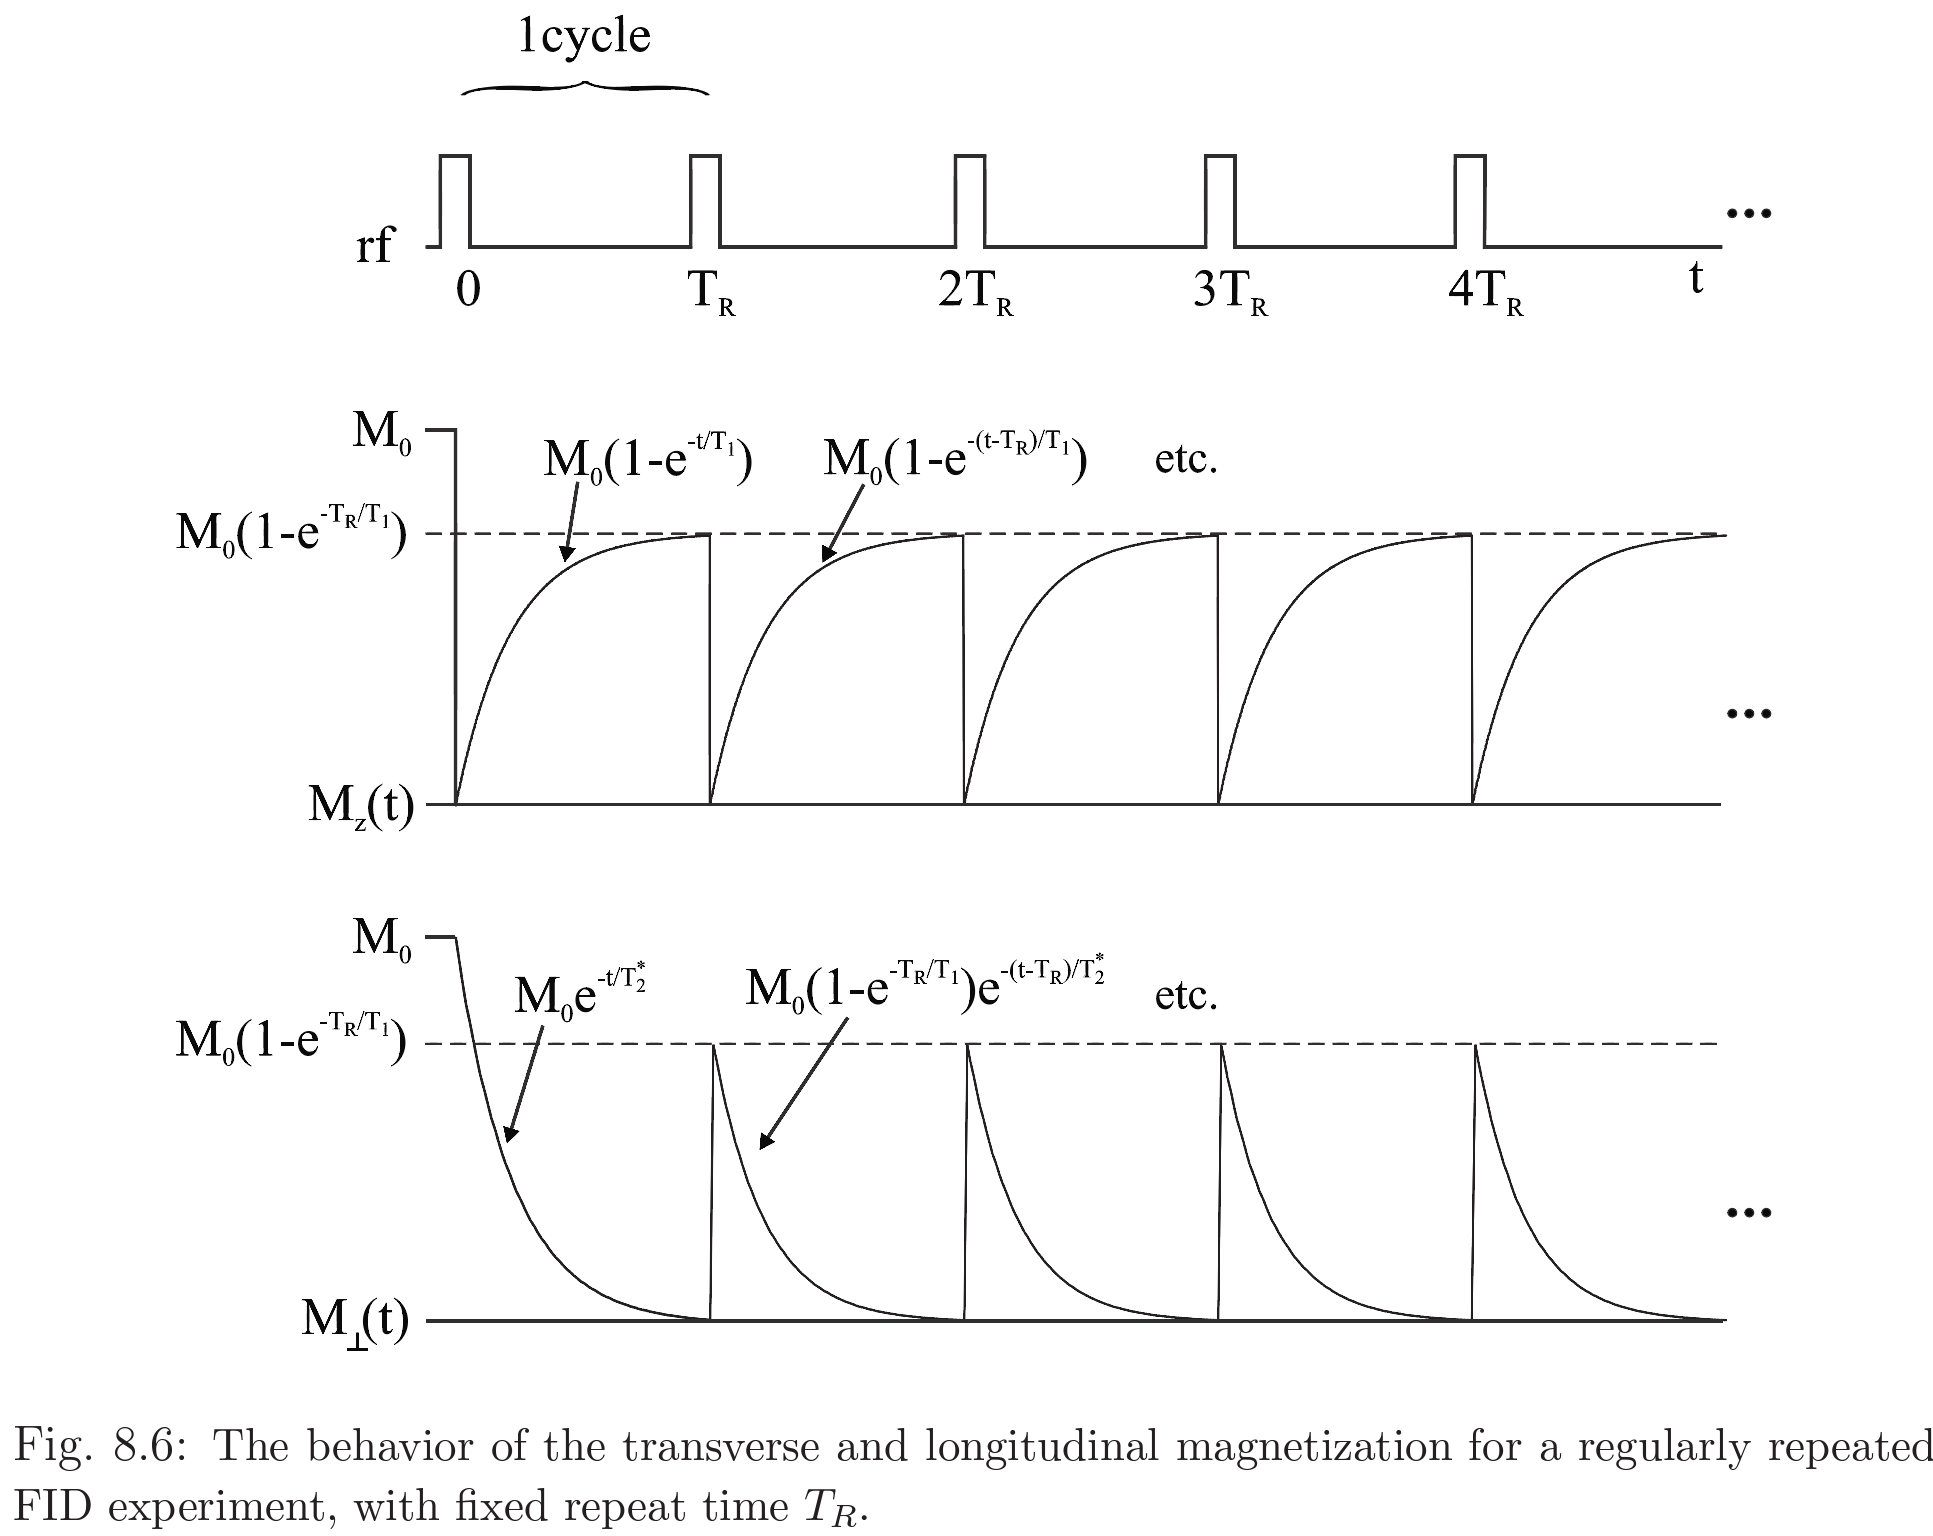
\includegraphics[trim={0cm 0cm 0 0},clip, keepaspectratio,width=0.4\textwidth]{FIDrep}\label{fig:FIDrep}\end{figure}
\end{block}
\end{frame}

\begin{frame}{$T_2*$ decay: dephasing of magnetization.}
%succo
\begin{align*}
&\frac{1}{T_2*}=\frac{1}{T_2}+\frac{1}{T_2'}\\
&M_+(\vec{r},t)=M_+(\vec{r},0)\exp{-\frac{t}{T_2*}}\\
&\phi(\vec{r},t)=-\gamma[B_0+\Delta B(\vec{r})]t
\end{align*}
$T_2'$ is machine/sample dependent $B_0$ inhomogeneities and is recoverable, $T_2$ is thermodynamic relaxing: $\sum_{sample}\exp{i\phi(\vec{r},t)}\to0$. Often $T_2'\ll T_2$.

\begin{block}{$T_2$ measure. Spin-echo.}
Impulso $(\pi/2)_{x'}$ determina spin (excess) lungo $y'$. $\Delta B(\vec{r})\neq0$ implica dephasing:
\begin{equation*}
\phi(\vec{r},t)=-\gamma\Delta B(\vec{r})t\quad 0\leq t\leq\tau
\end{equation*}
Applico impulso di $\pi$ attorno a $y'$:
\begin{align*}
&\phi(\vec{r},\tau+)=-\phi(\vec{r},\tau-)=\gamma\Delta B(\vec{r})\tau\\
&\phi(\vec{r},t)=-\phi(\vec{r},\tau)-\gamma\Delta B(\vec{r})(t-\tau)=-\gamma\Delta B(\vec{r})(t-t_E)
\end{align*}
\end{block}
\begin{block}{Misura $T_2$.}
%succo
\begin{align*}
&s(T_E)\propto\omega_0\exp{-\frac{T_E}{T_2}}\int d^3 rB_{\perp}M_{\perp}(\vec{r},0)\\
&T_2=\frac{T_E'-T_E}{\ln{[s(T_E)/s(T_E')]}}
\end{align*}
\end{block}
\end{frame}

\begin{wordonframe}{Spin-ECHO}
\begin{block}{Spin-echo exponential}
\begin{align*}
&(\TDy{t}{(M_+)})'=-R_2^{se}M_+\\
&R_2^{se}=\begin{pmatrix}R_2'+R_2\\-R_2'+R_2\\R_2'+R_2\end{pmatrix}\\
&M_{\perp}(t)=M_{\perp}(t_0)\exp{-(t-t_0)R_2^{se}}\\
&=M_{\perp}(0)\begin{pmatrix}\exp{-\frac{r}{T_2*}}\ 0<t<\tau\\\exp{-\frac{t}{T_2}}\exp{-\frac{(T_E-t)}{T_2'}}\ \tau<t<2\tau=T_E\\ \exp{-\frac{t}{T_2}}\exp{-\frac{(t-T_E)}{T_2'}}=\exp{-\frac{t}{T_2*}}\exp{-\frac{T_E}{T_2'}} \end{pmatrix}
\end{align*}
$T_2$ intrinsic rapid time fluctuation of local field.
\end{block}
Misure con $T_R\leq T_1$: ottimizzazione.
\end{wordonframe}

\begin{frame}[allowframebreaks]{Inversion recovery and $T_1$ measure - Spin-echo inversion recovery.}
Impulso $\pi$ attorno $x'$ e a $T_I$ di $\pi/2$
\begin{align*}
&M_z(0+)=-M_0\\
&M_z(t)=-M_0\exp{-\frac{t}{T_1}}+M_0(1-\exp{-\frac{t}{T_1}})\ 0<t<T_I\\
&\magort{}(t)=|M_0(1-2\exp{-\frac{T_I}{T_1}})|\exp{-\frac{(t-T_I)}{T_2*}}\\
&T_I^{null}=T_1\ln{2}
\end{align*}

\begin{figure}[!ht]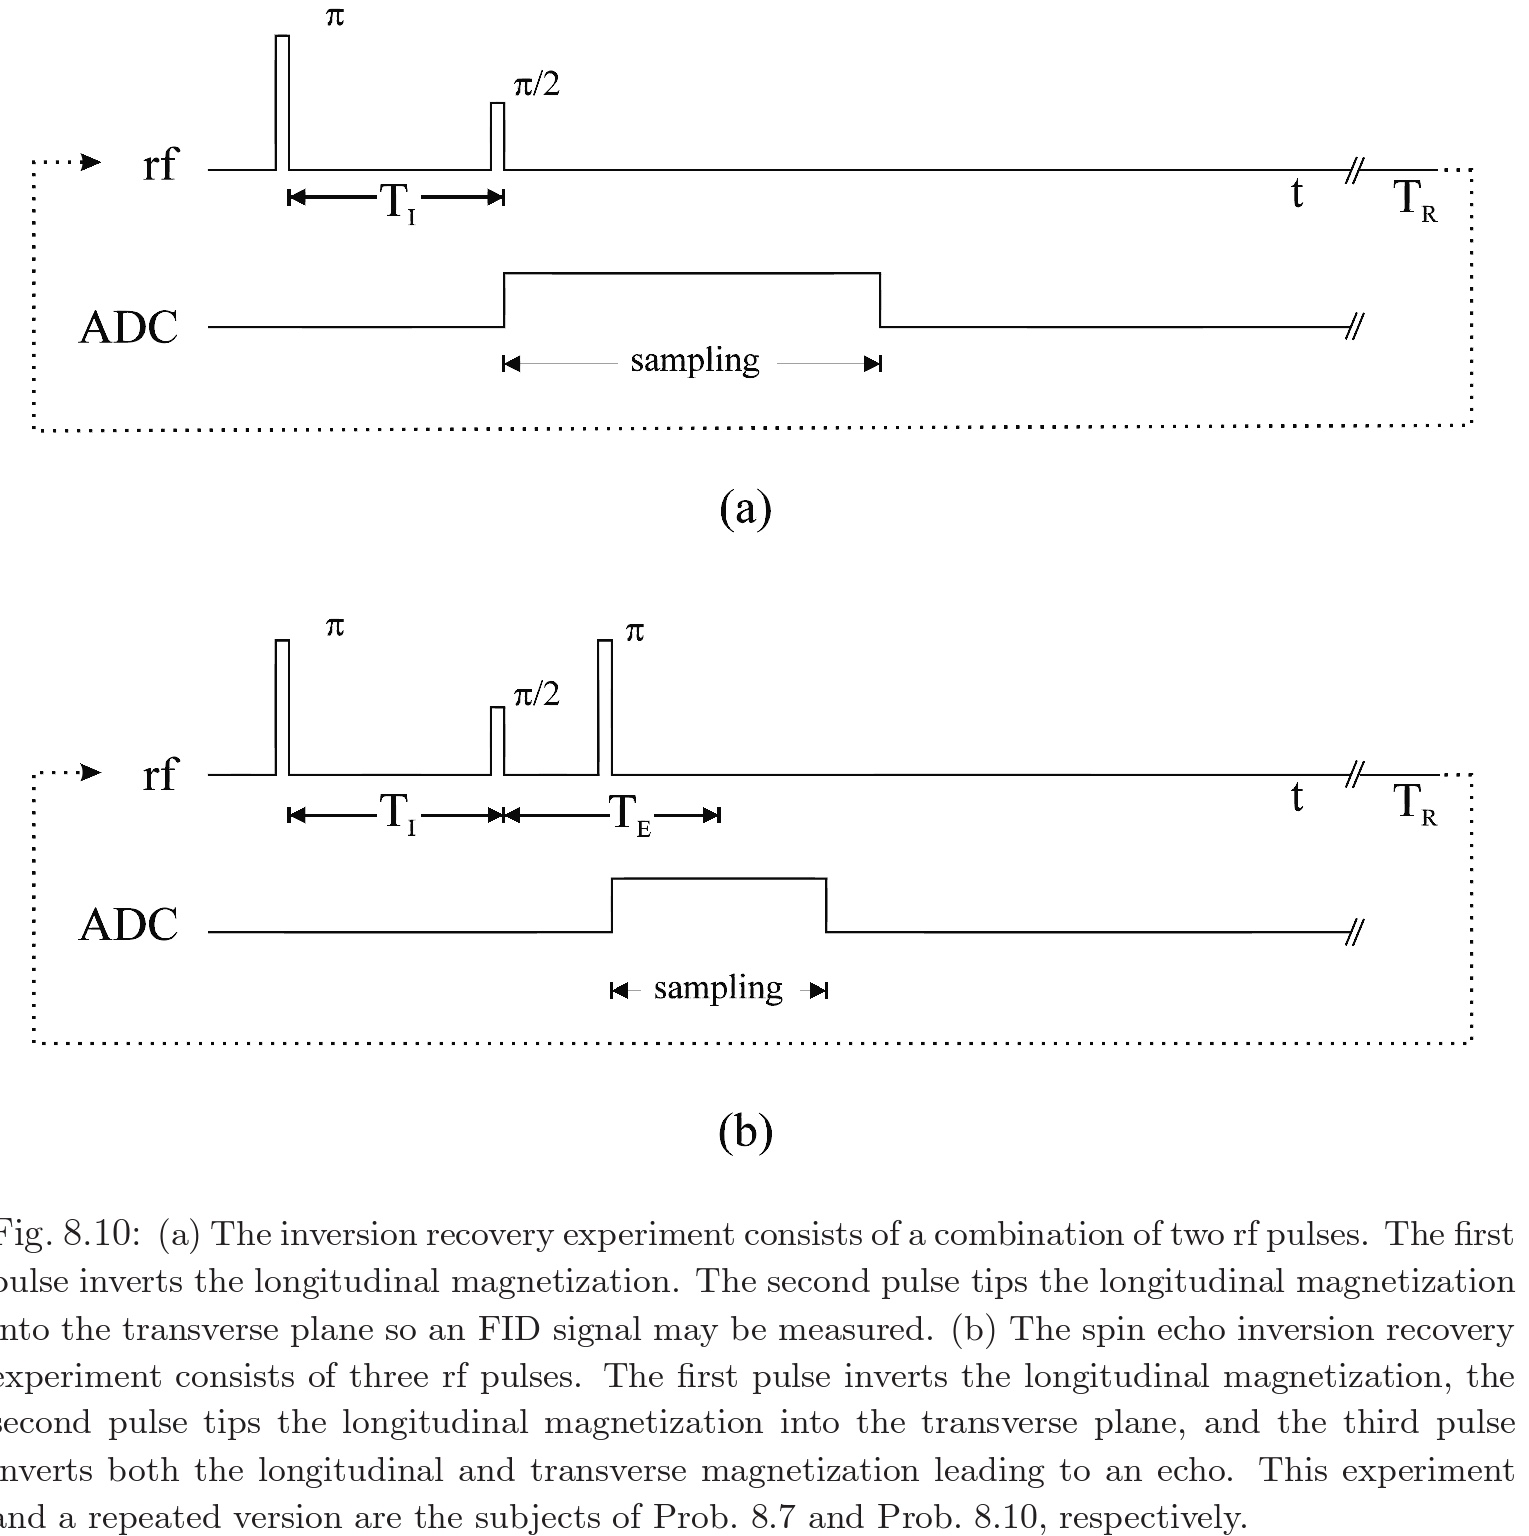
\includegraphics[trim={0cm 0 0 0},clip, width=0.9\textwidth]{IR-SE-sampling}
\label{fig:IR-SE-sampling}\end{figure} 
\begin{figure}[!ht]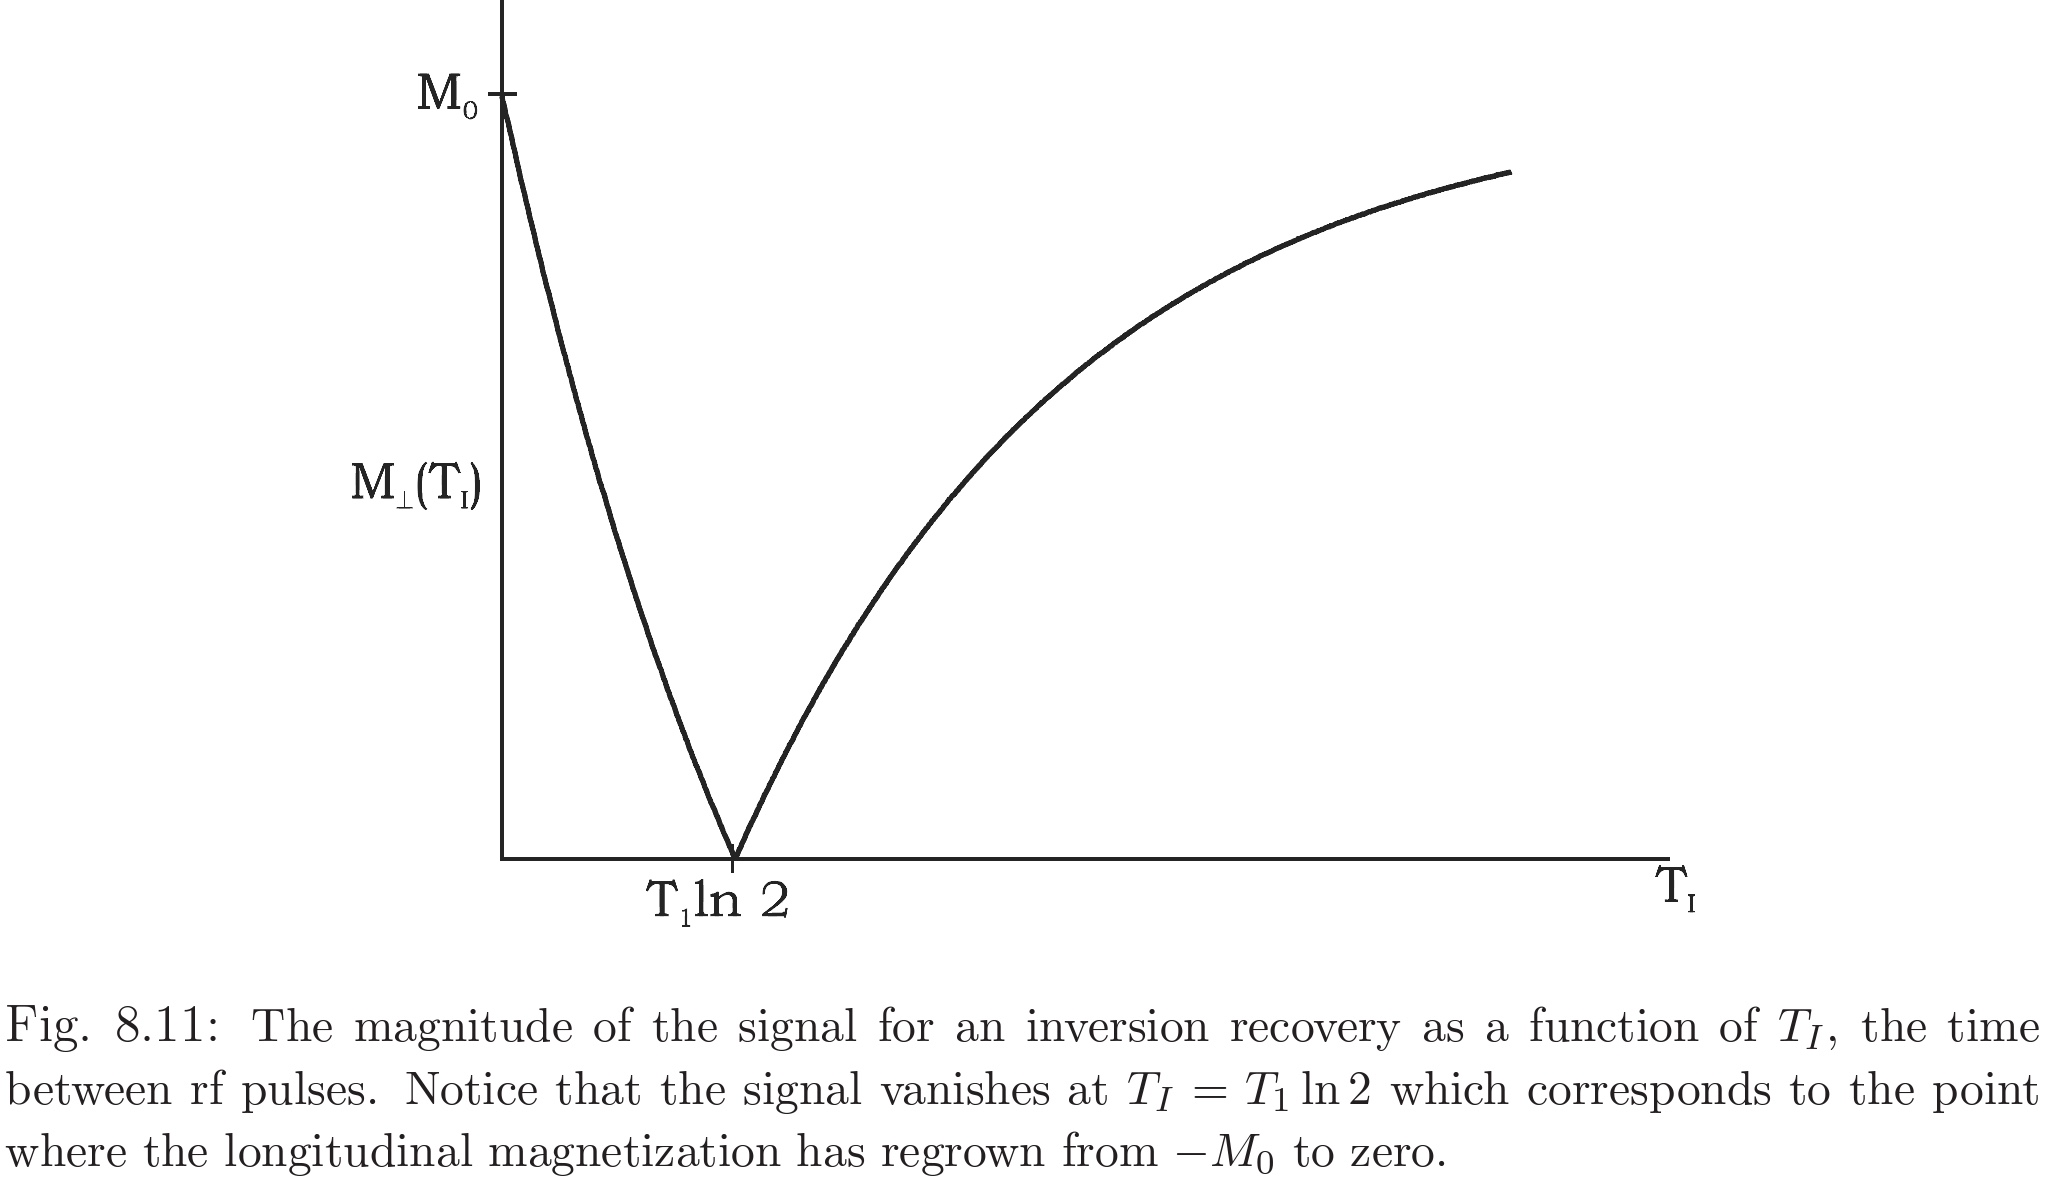
\includegraphics[trim={0cm 0 0 0},clip,width=0.9\textwidth]{IRvsTI}
\label{fig:IRvsTI}
\end{figure}

\end{frame}

\begin{frame}{Chemical shift and NMR spectroscopy}
%succo
Broadband RF excitation: complicated FID signal
\begin{align*}
&\omega_{0i}=\gamma_iB_0
\end{align*}
Determinazioni specie nucleari nel campione (excited by pulse spectrum).
Shielding constant: linear response of electrons to $B_{ext}$:
\begin{align*}
&B_{shift}(j)=(1-\sigma_j)B_0\to f_{\sigma}=-\sigma\gammabar B_0\\
&s(t)=\sum_jN_j\exp{i\gamma\sigma_jB_0t}
\end{align*}
\end{frame}

\section{Imaging: phase encoding, k-spazio, imaging equation}\linkdest{imaging}

\begin{frame}[allowframebreaks]{Fourier imaging, gradient echo and K-space}
Rilassamento dopo $\pi/2$-pulse:$M_{\perp}=M_0(\vec{r})$.
\begin{block}{Aggiungo campo che varia linearmente lungo z}
%succo
\begin{align*}
&s(t)\propto\int d^3 r\rho(\vec{r})\exp{i[\Omega t+\phi(\vec{r},t)]}\\
&B_z(z,t)=B_0+zG(t)\ \Rightarrow\ \omega=\omega_0+\omega_G(z,t)
\end{align*}
Frequency encoding: $\omega_G=\gamma zG(t)$.
\begin{equation*}
\phi_G(z,t)=-\int_0^td t'\omega_G(z,t')=-\gamma z\int_0^td t'G(t)
\end{equation*}
\end{block}
\begin{block}{1D imaging equation}
%succo
\begin{equation*}
s(t)=\int d z\rho(z)\exp{i\phi_G(z,t)}
\end{equation*}
$\rho$ effective spin density
\end{block}
\begin{figure}[!ht]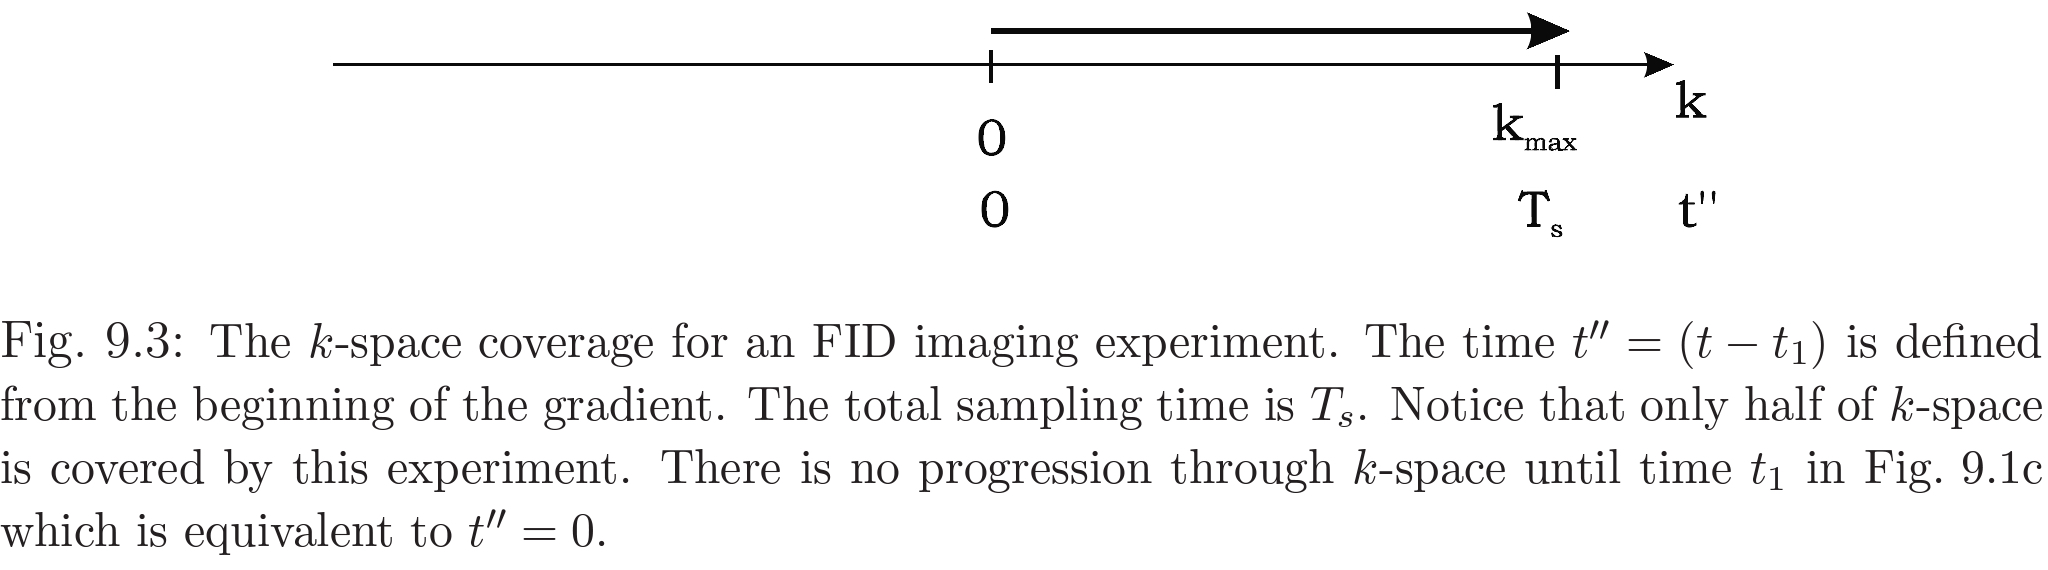
\includegraphics[trim={0cm 0cm 0 0},clip, keepaspectratio,width=\textwidth]{FID-k}\label{fig:FID-k}\end{figure}
\end{frame}

\begin{wordonframe}{Effective spin density}
\begin{align*}
M_0=\frac{1}{4}\rho_0(\vec{r})\frac{\gamma^2\hbar^2}{KT}\\
\rho(\vec{r})=\omega_0\Lambda B_{\perp}M_0
\end{align*}
\end{wordonframe} 

\begin{frame}{K-spazio}
\begin{align*}
s(k)=\int d z\rho(z)\exp{-i2\pi kz}
\end{align*}
Per gradiente uniforma lungo z $s(k)$ \'e la trasformata di Fourier della "densit\'a effettiva di spin del campione.
\begin{block}{Antitrasformata del segnale \'e la densit\'a spaziale}
\begin{equation*}
\rho(z)=\int d ks(k)\exp{i2\pi kz}
\end{equation*}
\end{block}
\begin{block}{Coverage of K-space}
Campionamento uniforme: sampling at constant rate in presence of constant gradient.
\begin{equation*}
k=\gammabar\int_0^tG(t')d t'
\end{equation*}
\end{block} 
\end{frame}

\begin{frame}{two spin system}
Two spin at $z=\pm z_0$: in rotating frame they preceed clock/anticlock-wise.
\begin{align*}
&\phi(\pm z_0,t)=\mp\gamma Gz_0(t-t_1)\\
&s(t)=s_0[\exp{-i\gamma Gz_0t}+\exp{i\gamma Gz_0t}]\\
&=2s_0\cos{(\gamma G t z_0)}=2s_0\cos{(2\pi kz_0)}\\
&0\leq t\leq t_2:\ 0\leq k\leq k_2=\gammabar Gt_2
\rho(z)=\intsinf{}d k2s_0\cos{(2pi kz_0)}\exp{i2\pi kz}\\
&=s_0[\delta(z+z_0)+\delta(z-z_0)]
\end{align*}

\end{frame}

\begin{frame}{Gradient echo}
%succo
\begin{figure}[!ht]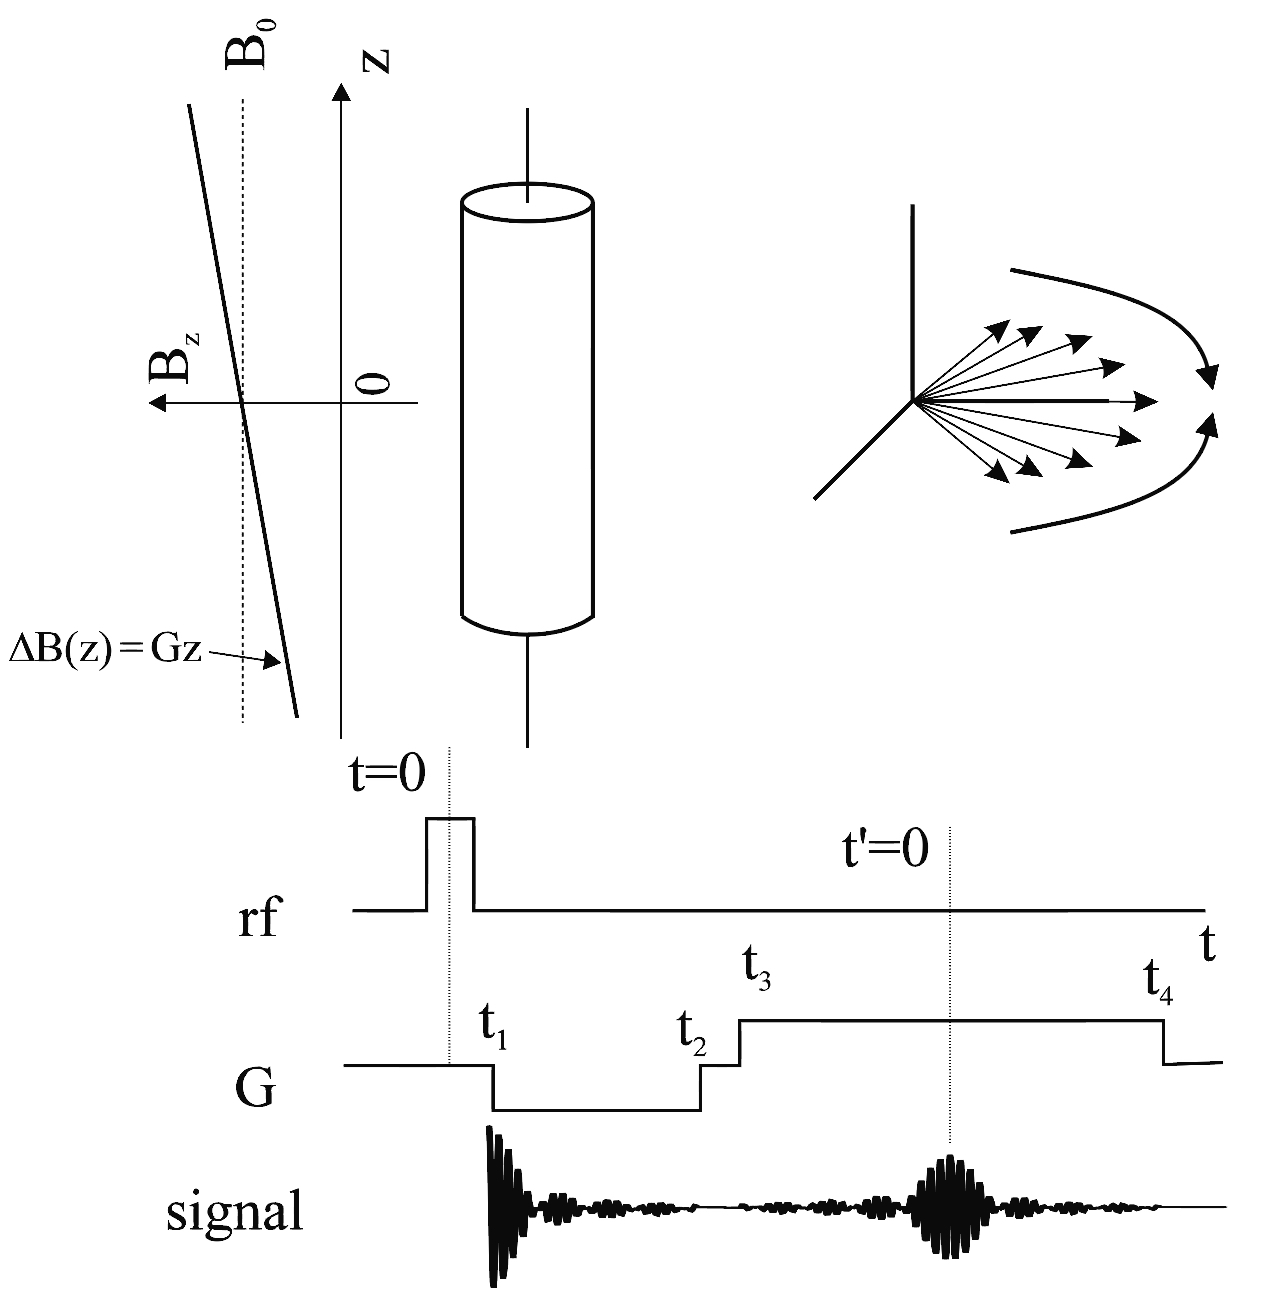
\includegraphics[trim={0cm 0cm 0 0},clip, keepaspectratio,height=0.9\textheight]{GEimaging}\end{figure}

\end{frame}

\begin{wordonframe}{Gradient echo}
\begin{align*}
&s(t')=\int d z\rho(z)\exp{-i\gamma Gzt'}:\ -\frac{t_4-t_3}{2}\leq t'\leq \frac{t_4-t_3}{2}
\end{align*}
\end{wordonframe}

\begin{frame}[allowframebreaks]{Spin-echo imaging}
%succo
\begin{figure}[!ht]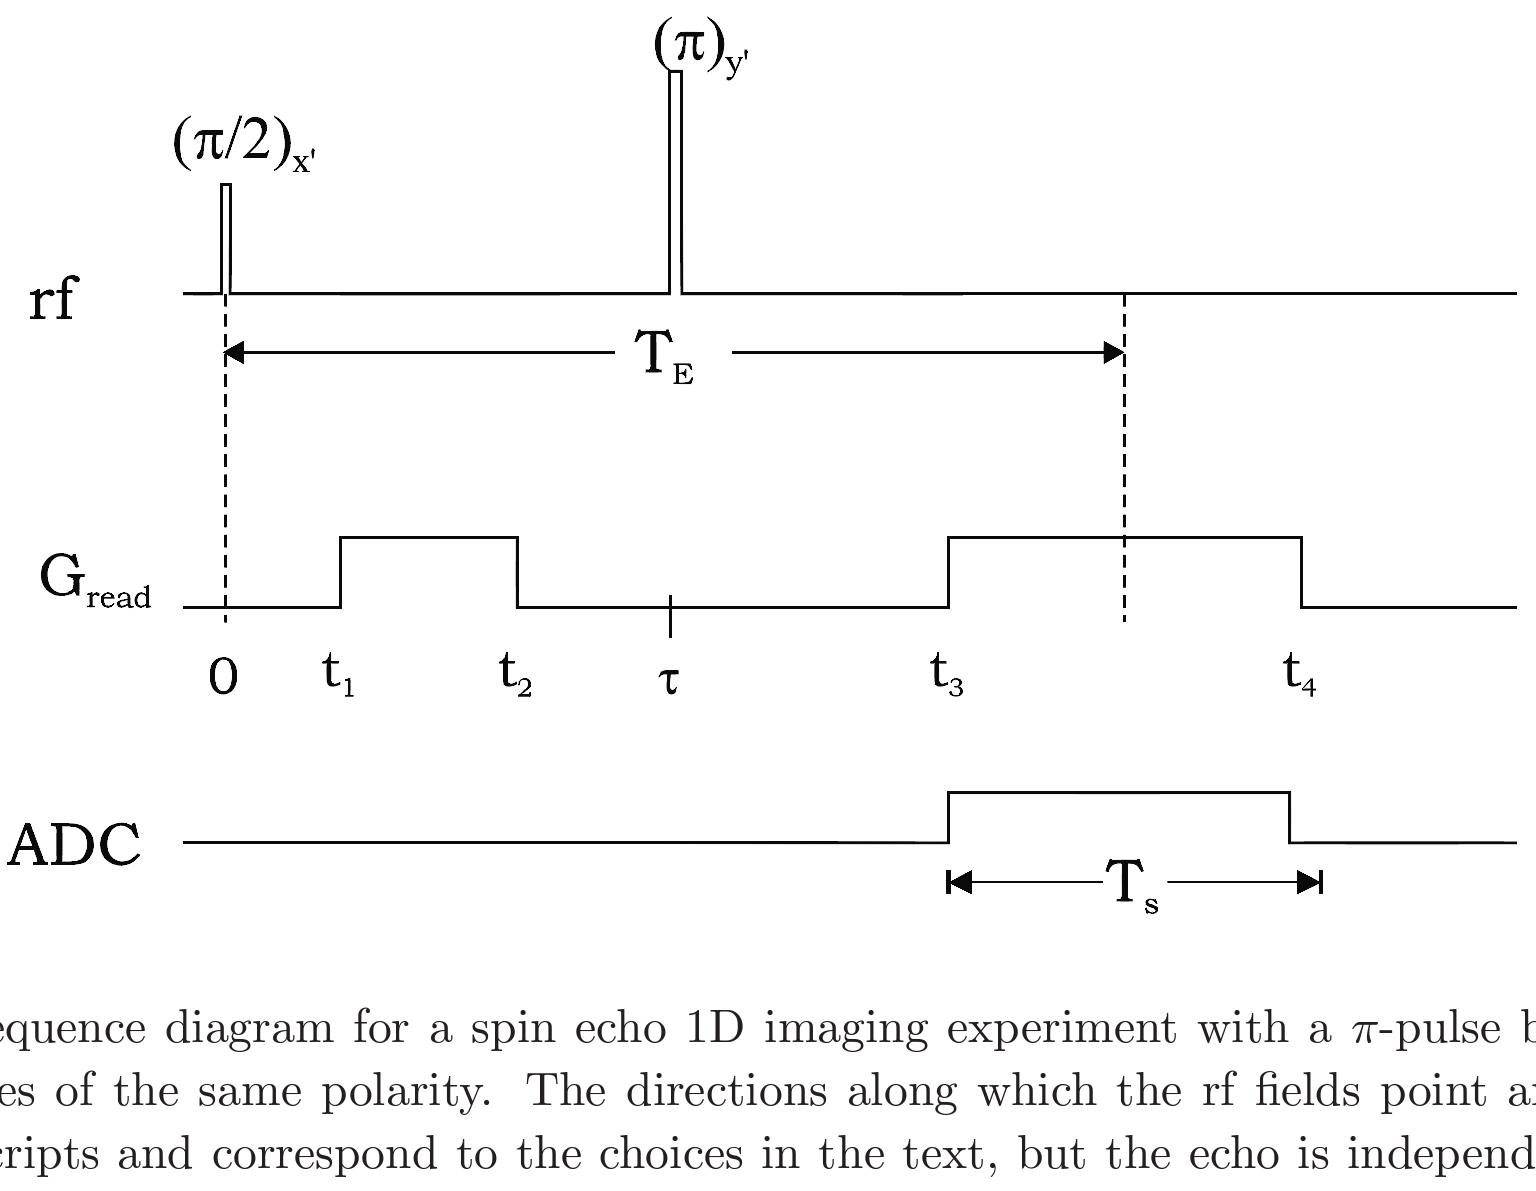
\includegraphics[trim={0cm 0cm 0 0},clip, keepaspectratio,height=0.45\textheight]{SEimaging}\end{figure}
\begin{figure}[!ht]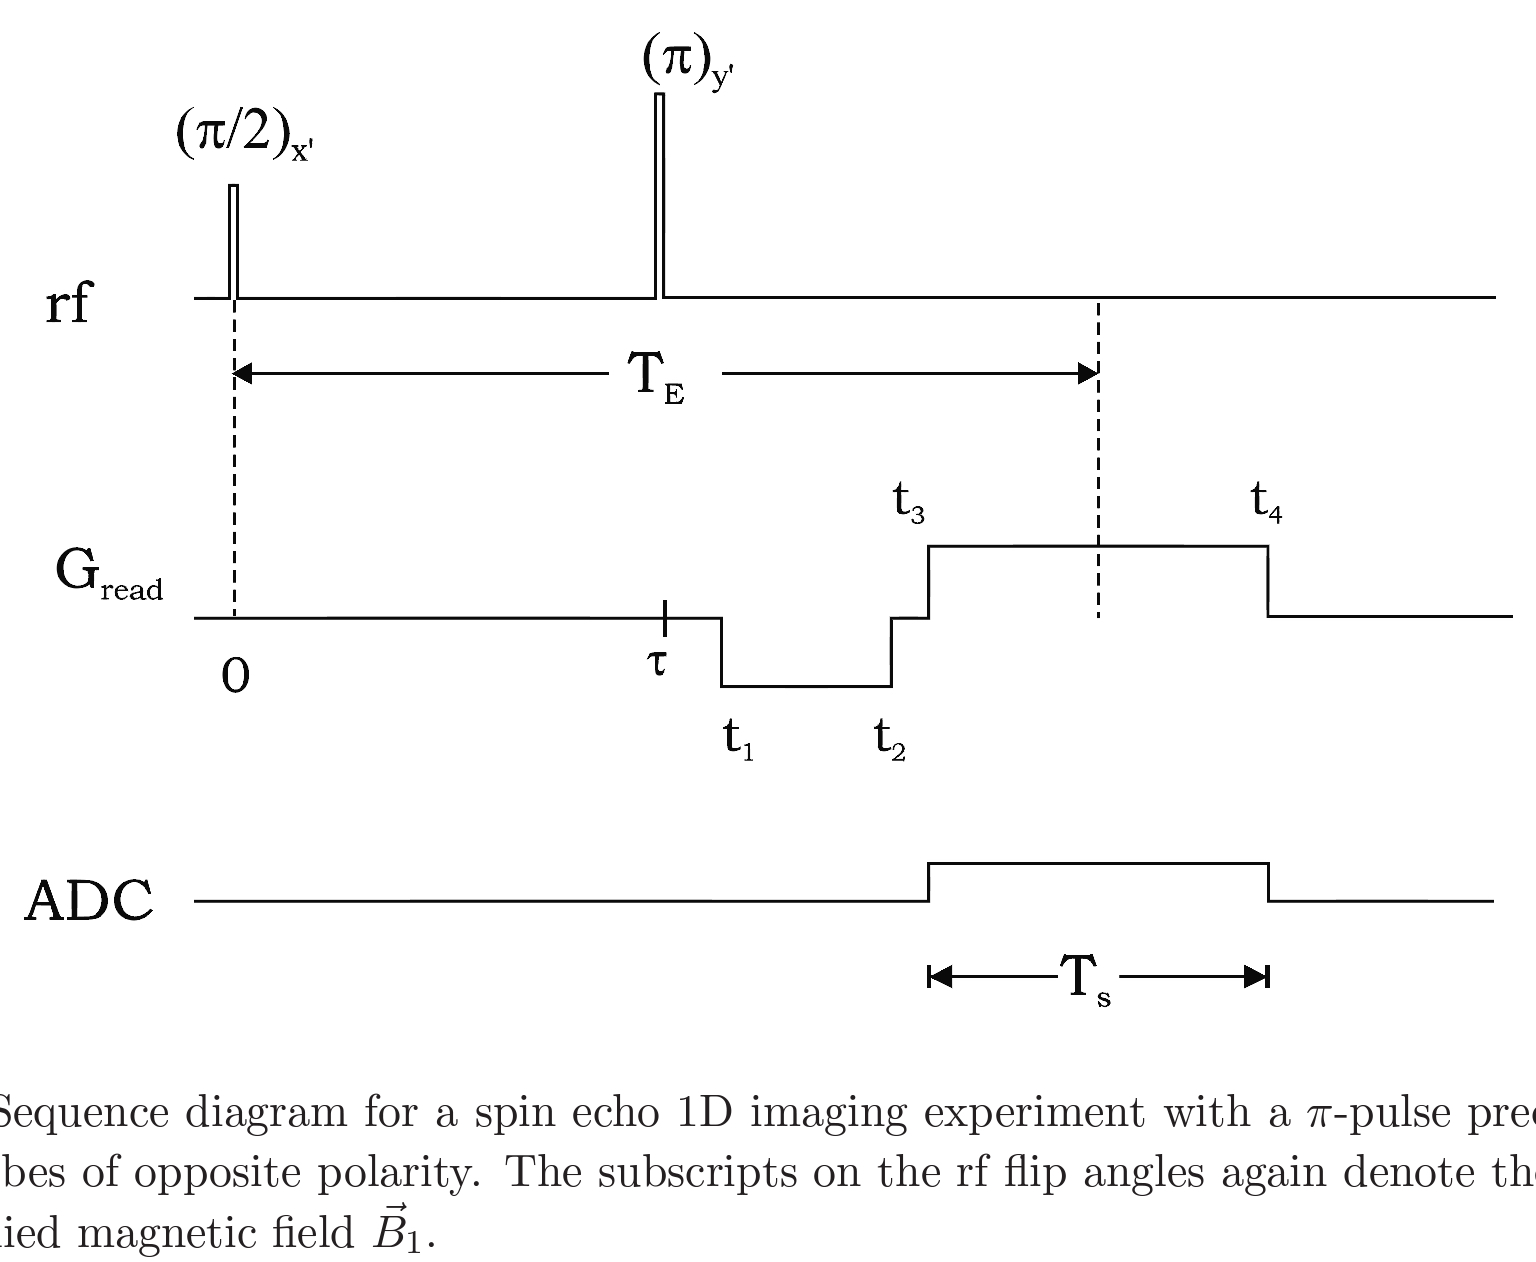
\includegraphics[trim={0cm 0cm 0 0},clip, keepaspectratio,height=0.45\textheight]{SEtotimaging}\end{figure}
\end{frame}

\begin{wordonframe}{Spin echo imaging}
Gradient echo refocus phase induced by gradient but does NOT refocus dephasing due static field inhomogeneities.

\begin{align*}
&\phi(z,t)=-\gamma\Delta B(z)t-\gamma Gz(t-t_1):\ t_1<t<t_2\\
&(\pi)_{y'},\ t=\tau:\ \phi\to-\phi\\
&\phi(z,t)=\gamma\Delta B(z)\tau+\gamma Gz(t_2-t_1)-\gamma\Delta B(z)(t-\tau)\\
&-\gamma Gz(t-t_3):\ t_3<t<t_4
\end{align*}
Total phase induced by $B_0/G$ inhomogeneities has been refocused.
Si ha:
\begin{align*}
&\phi(z,T_E)=0:\ 2\tau=t_3+(t_2-t_1)
\end{align*}
\end{wordonframe}


\begin{frame}{K-space coverage}
\begin{figure}[!ht]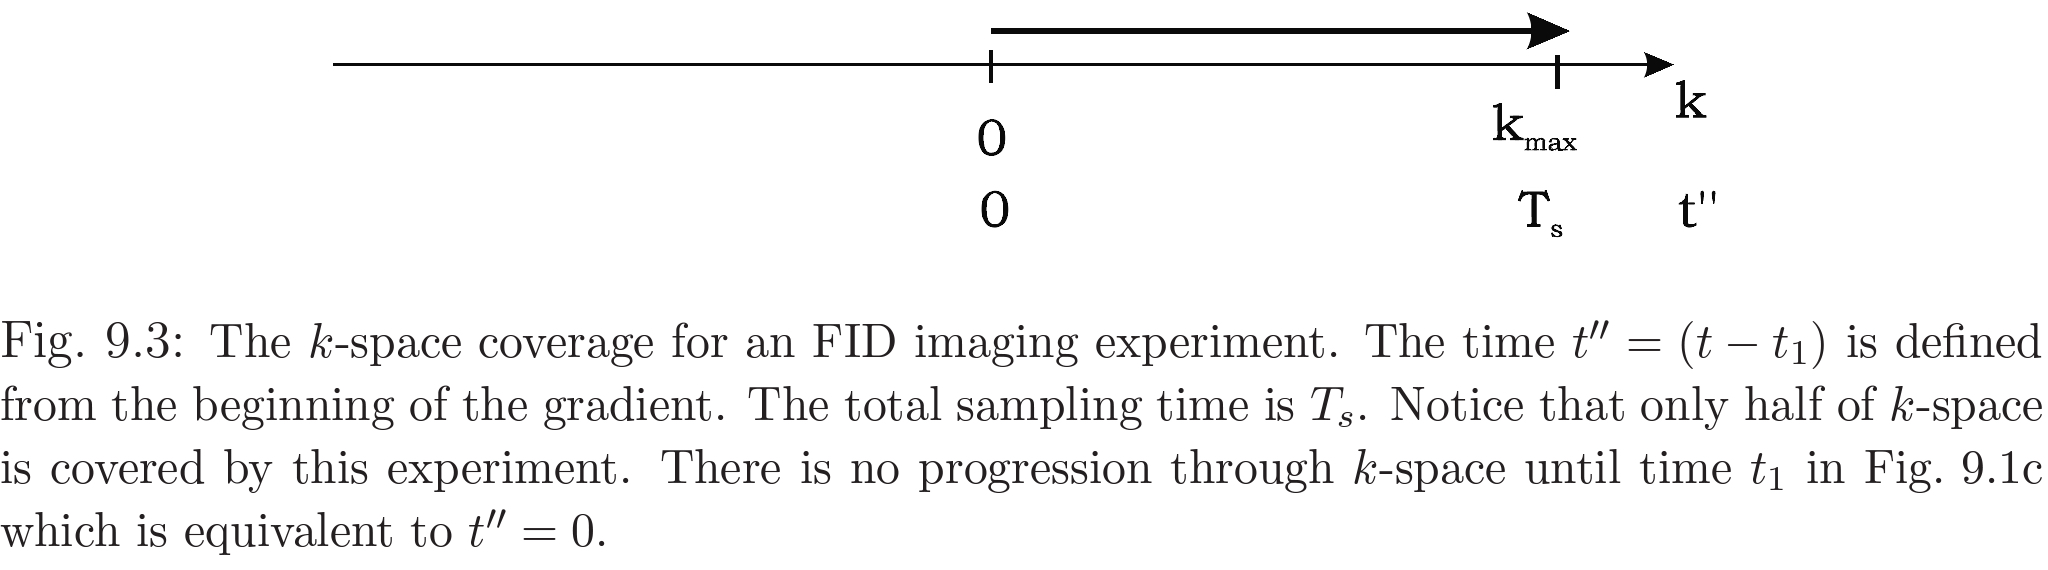
\includegraphics[trim={0cm 5cm 0 0},clip, keepaspectratio,height=0.3\textheight]{FID-k}\end{figure}

\begin{figure}[!ht]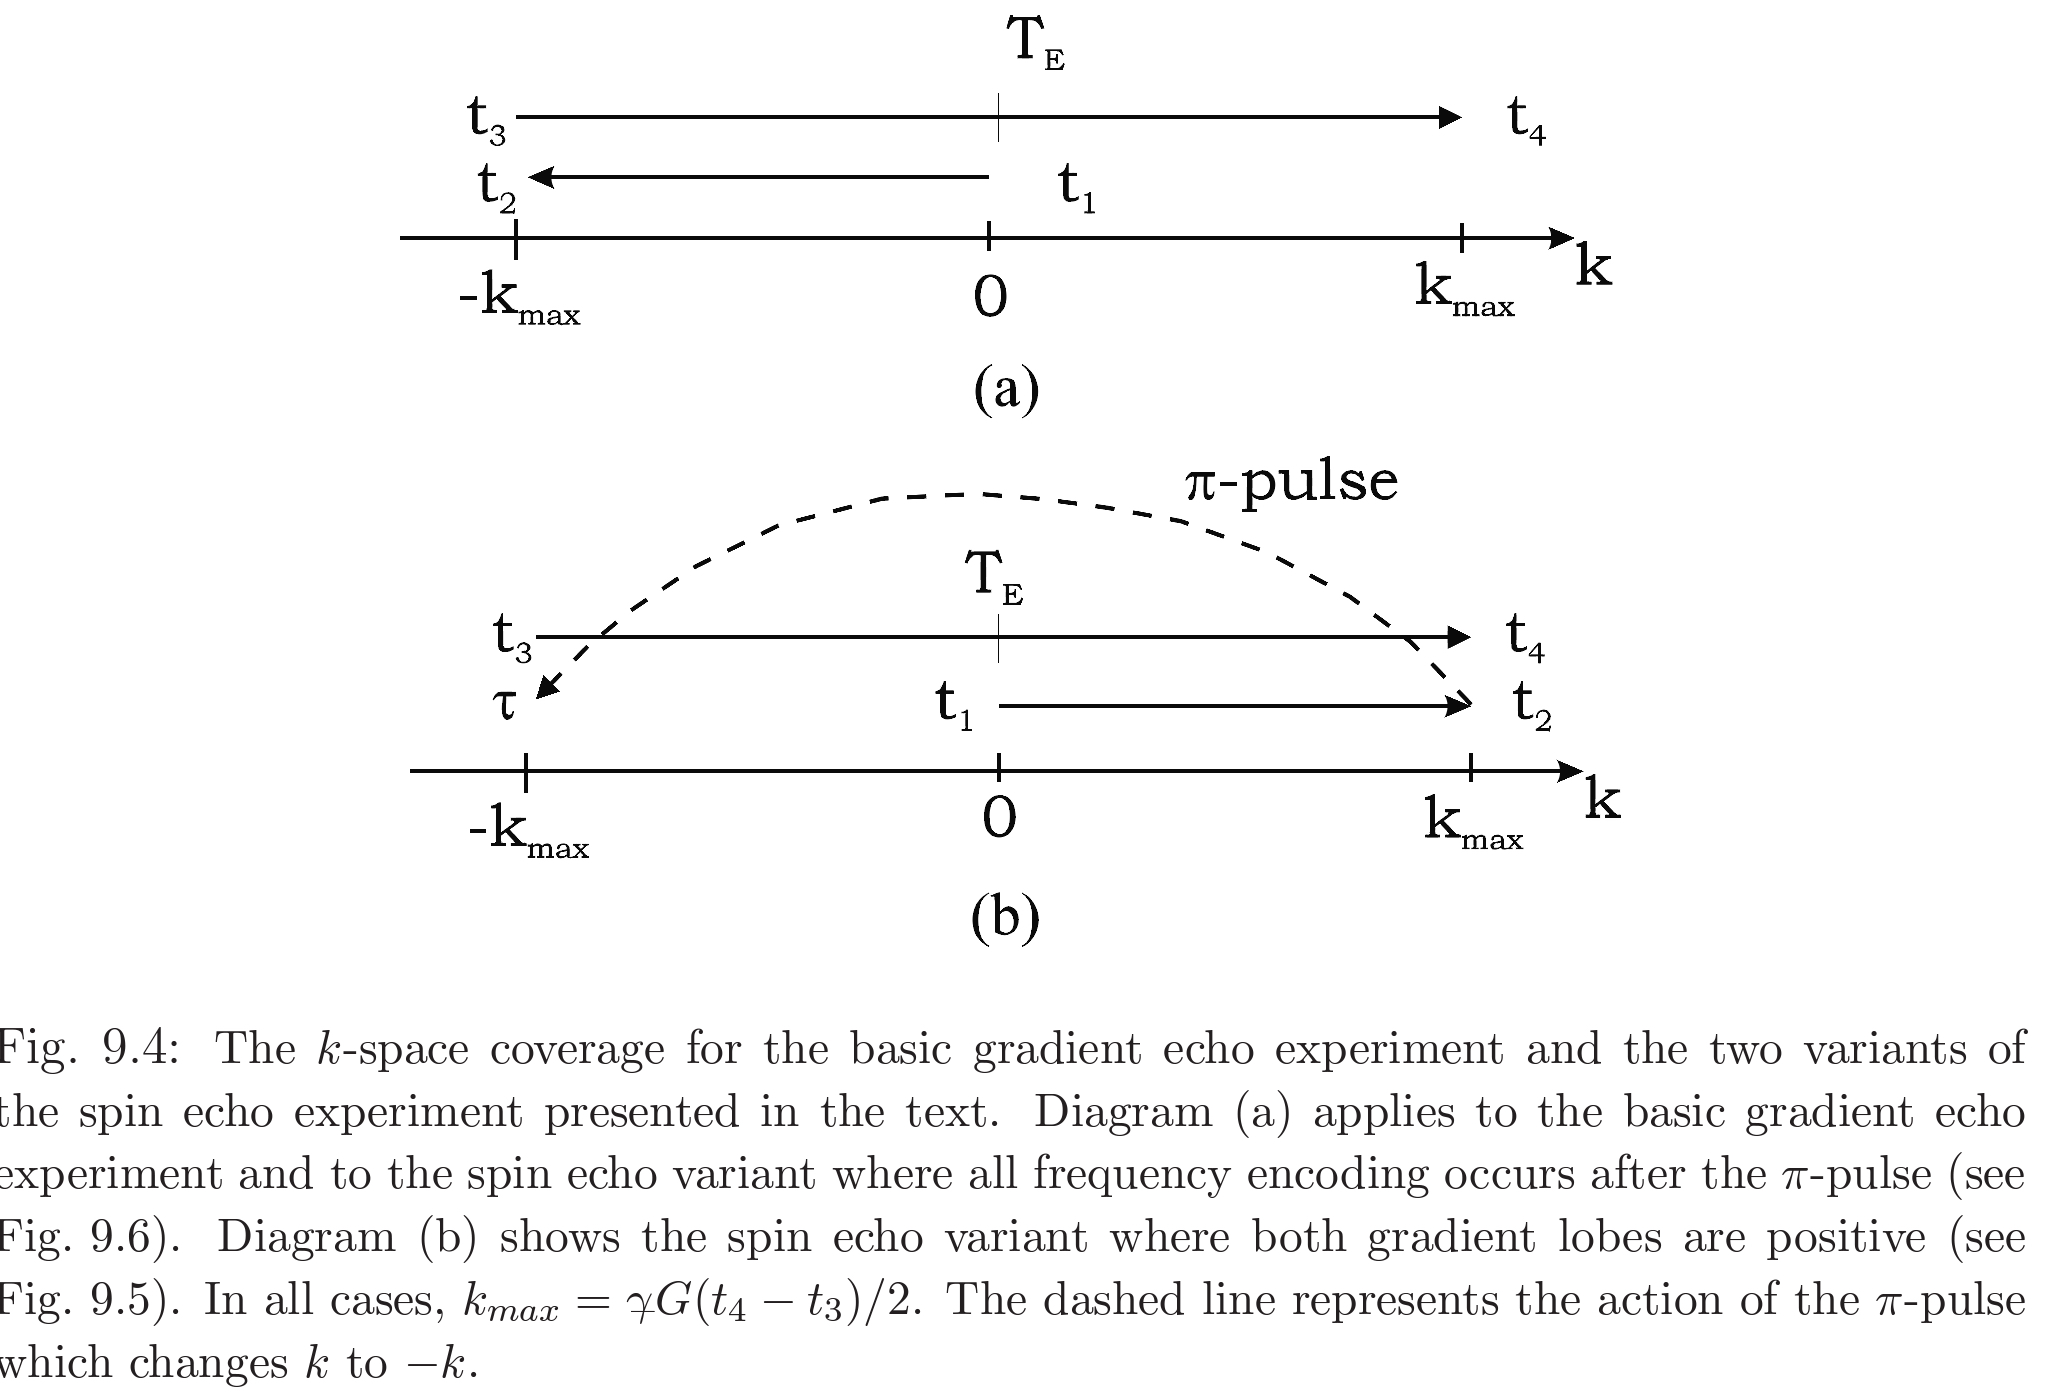
\includegraphics[trim={0cm 0cm 0 0},clip, keepaspectratio,height=0.6\textheight]{SE-GE-k}\end{figure}
\end{frame}

\begin{frame}[allowframebreaks]{Imaging in 3D: 3D imaging  vs 2D multislice imaging}
\begin{block}{3D imaging}
\begin{figure}[!ht]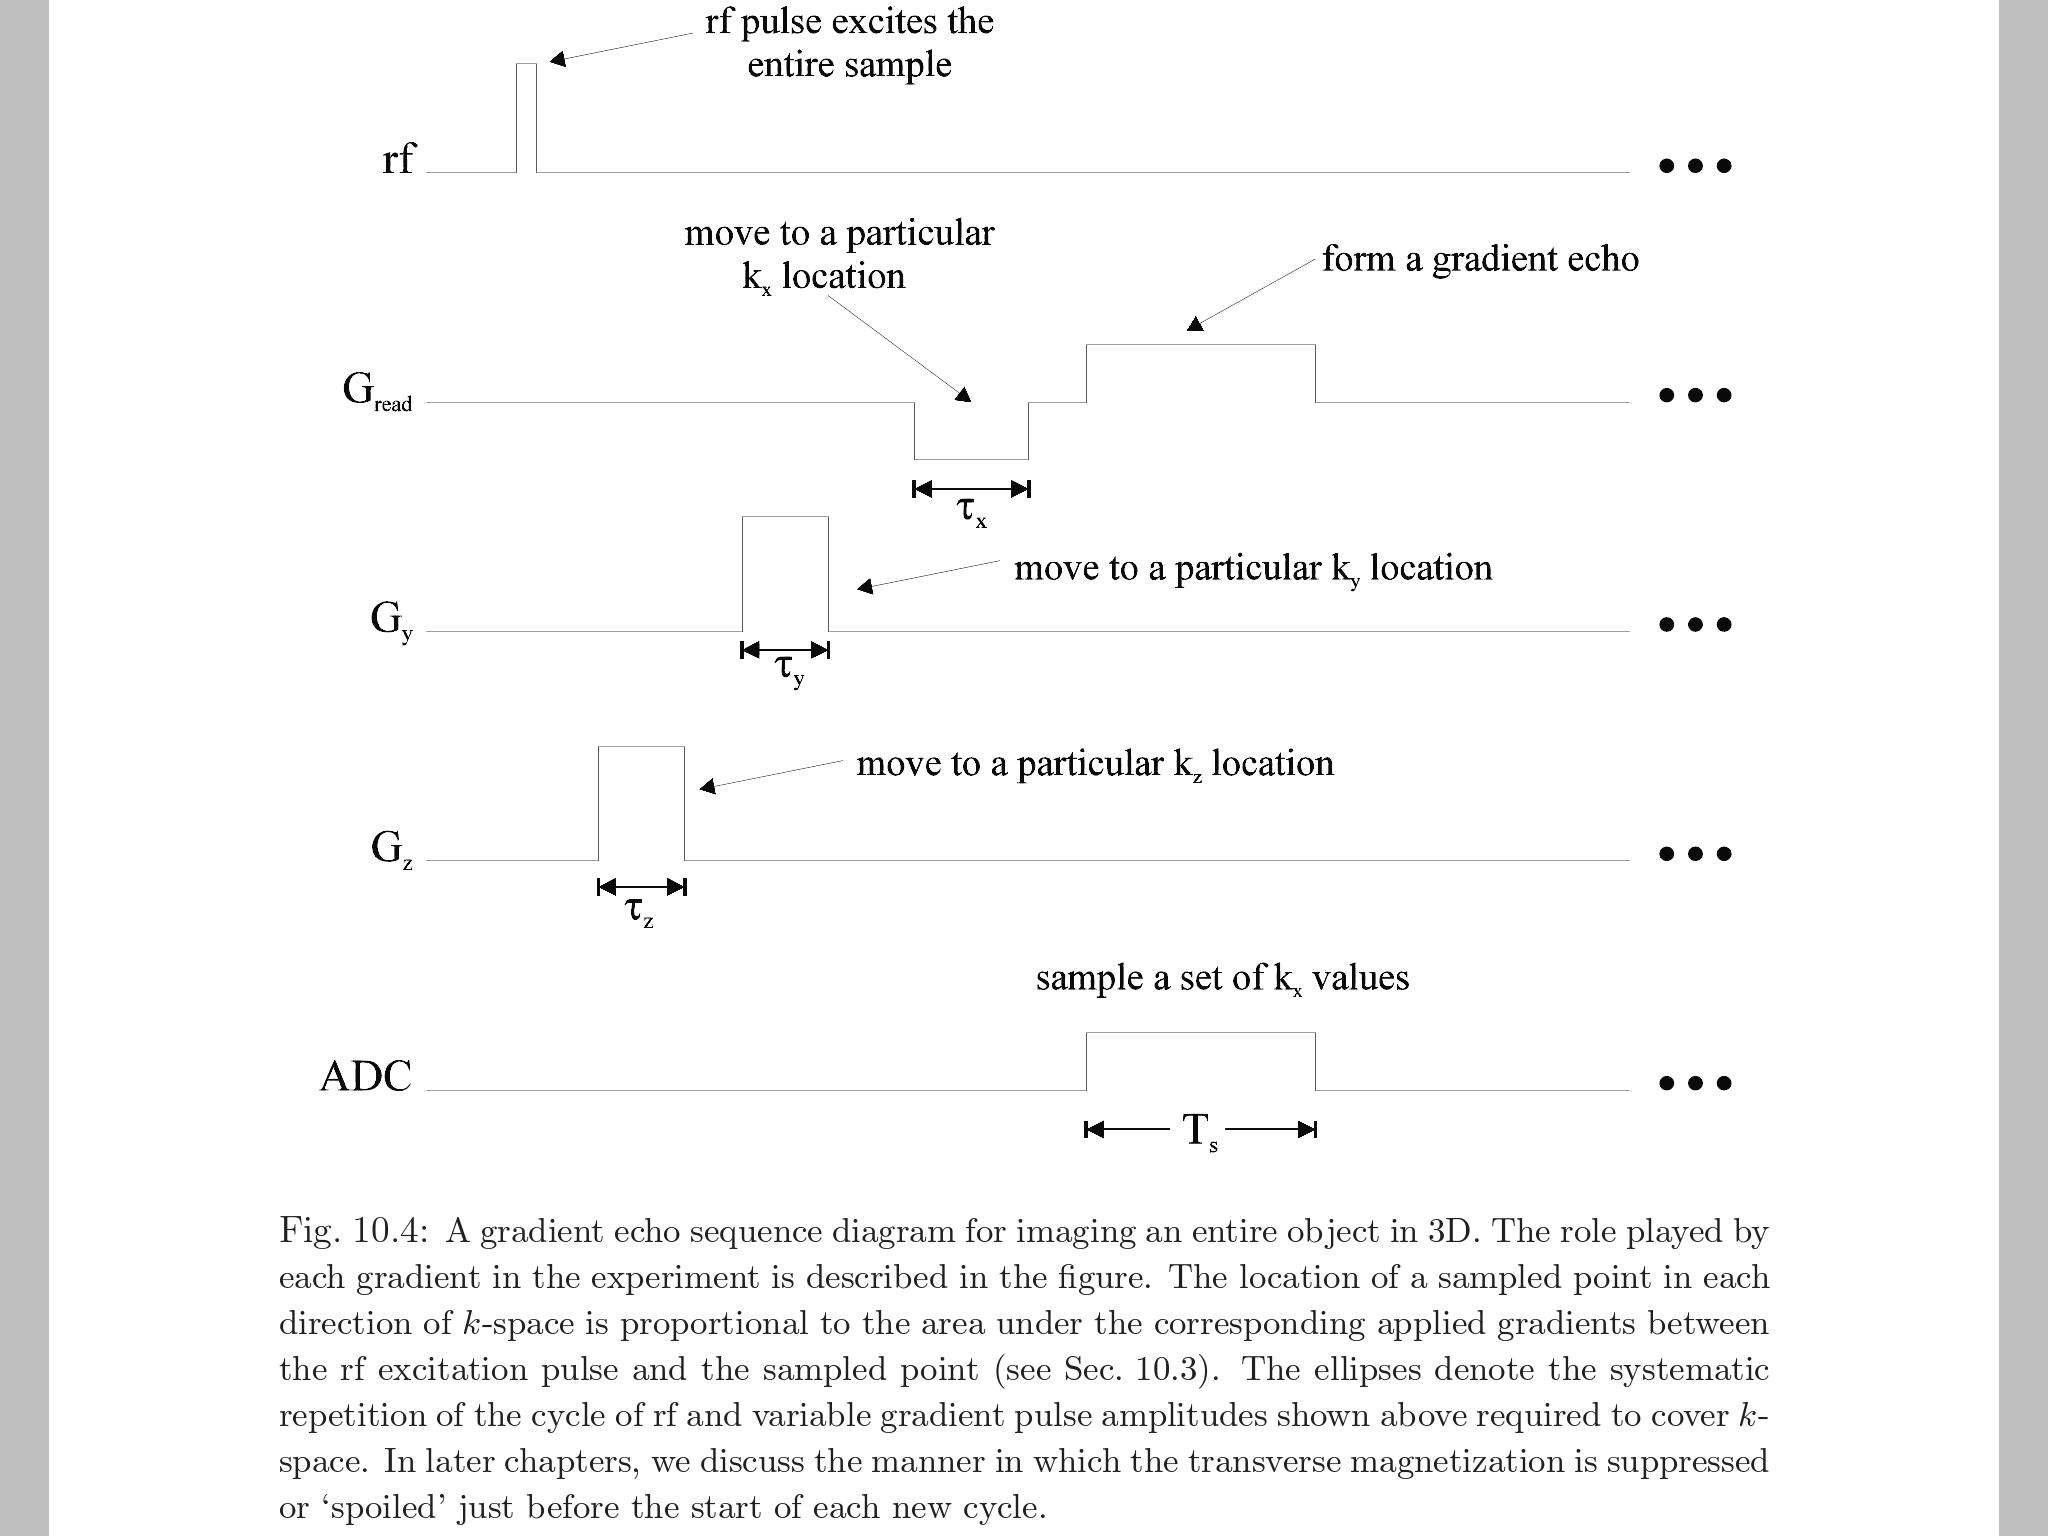
\includegraphics[trim={0cm 0cm 0 0},clip, keepaspectratio,height=0.5\textheight]{3Dimaging}\label{fig:3Dimaging}\end{figure}
\begin{align*}
&s(\vec{k})=\int d^3 r\rho(\vec{r})\exp{-i2\pi \scap{k}{r}}\\
&k_i(t)=\gammabar\int_0^tG_i(t')d t'\\
&\mathcal{F}s(\vec{k})\propto\rho(\vec{r})
\end{align*}
\end{block}
\begin{block}{2D multi-slice imaging}
Slice selection, $f(z)=f_0+\gammabar G_zz$: $z_0\pm\frac{\Delta z}{2}$ quindi $f_{RF}=\gammabar G_zz_0-\gammabar G_z\frac{\Delta z}{2}\gammabar G_zz_0+\gammabar G_z\frac{\Delta z}{2}$, cio\'e $BW_{RF}=\Delta f$. Imponiamo che nella slice il flip-angle sia uniforme
\begin{align*}
&RF(f)=\rect{\frac{\Delta f}{f}}:\ -\gammabar G_z\frac{\Delta z}{2}\leq f\leq \gammabar G_z\frac{\Delta z}{2}\\
&B_1(t)=\sinc{(\pi\Delta f t)}
\end{align*}

\begin{figure}[!ht]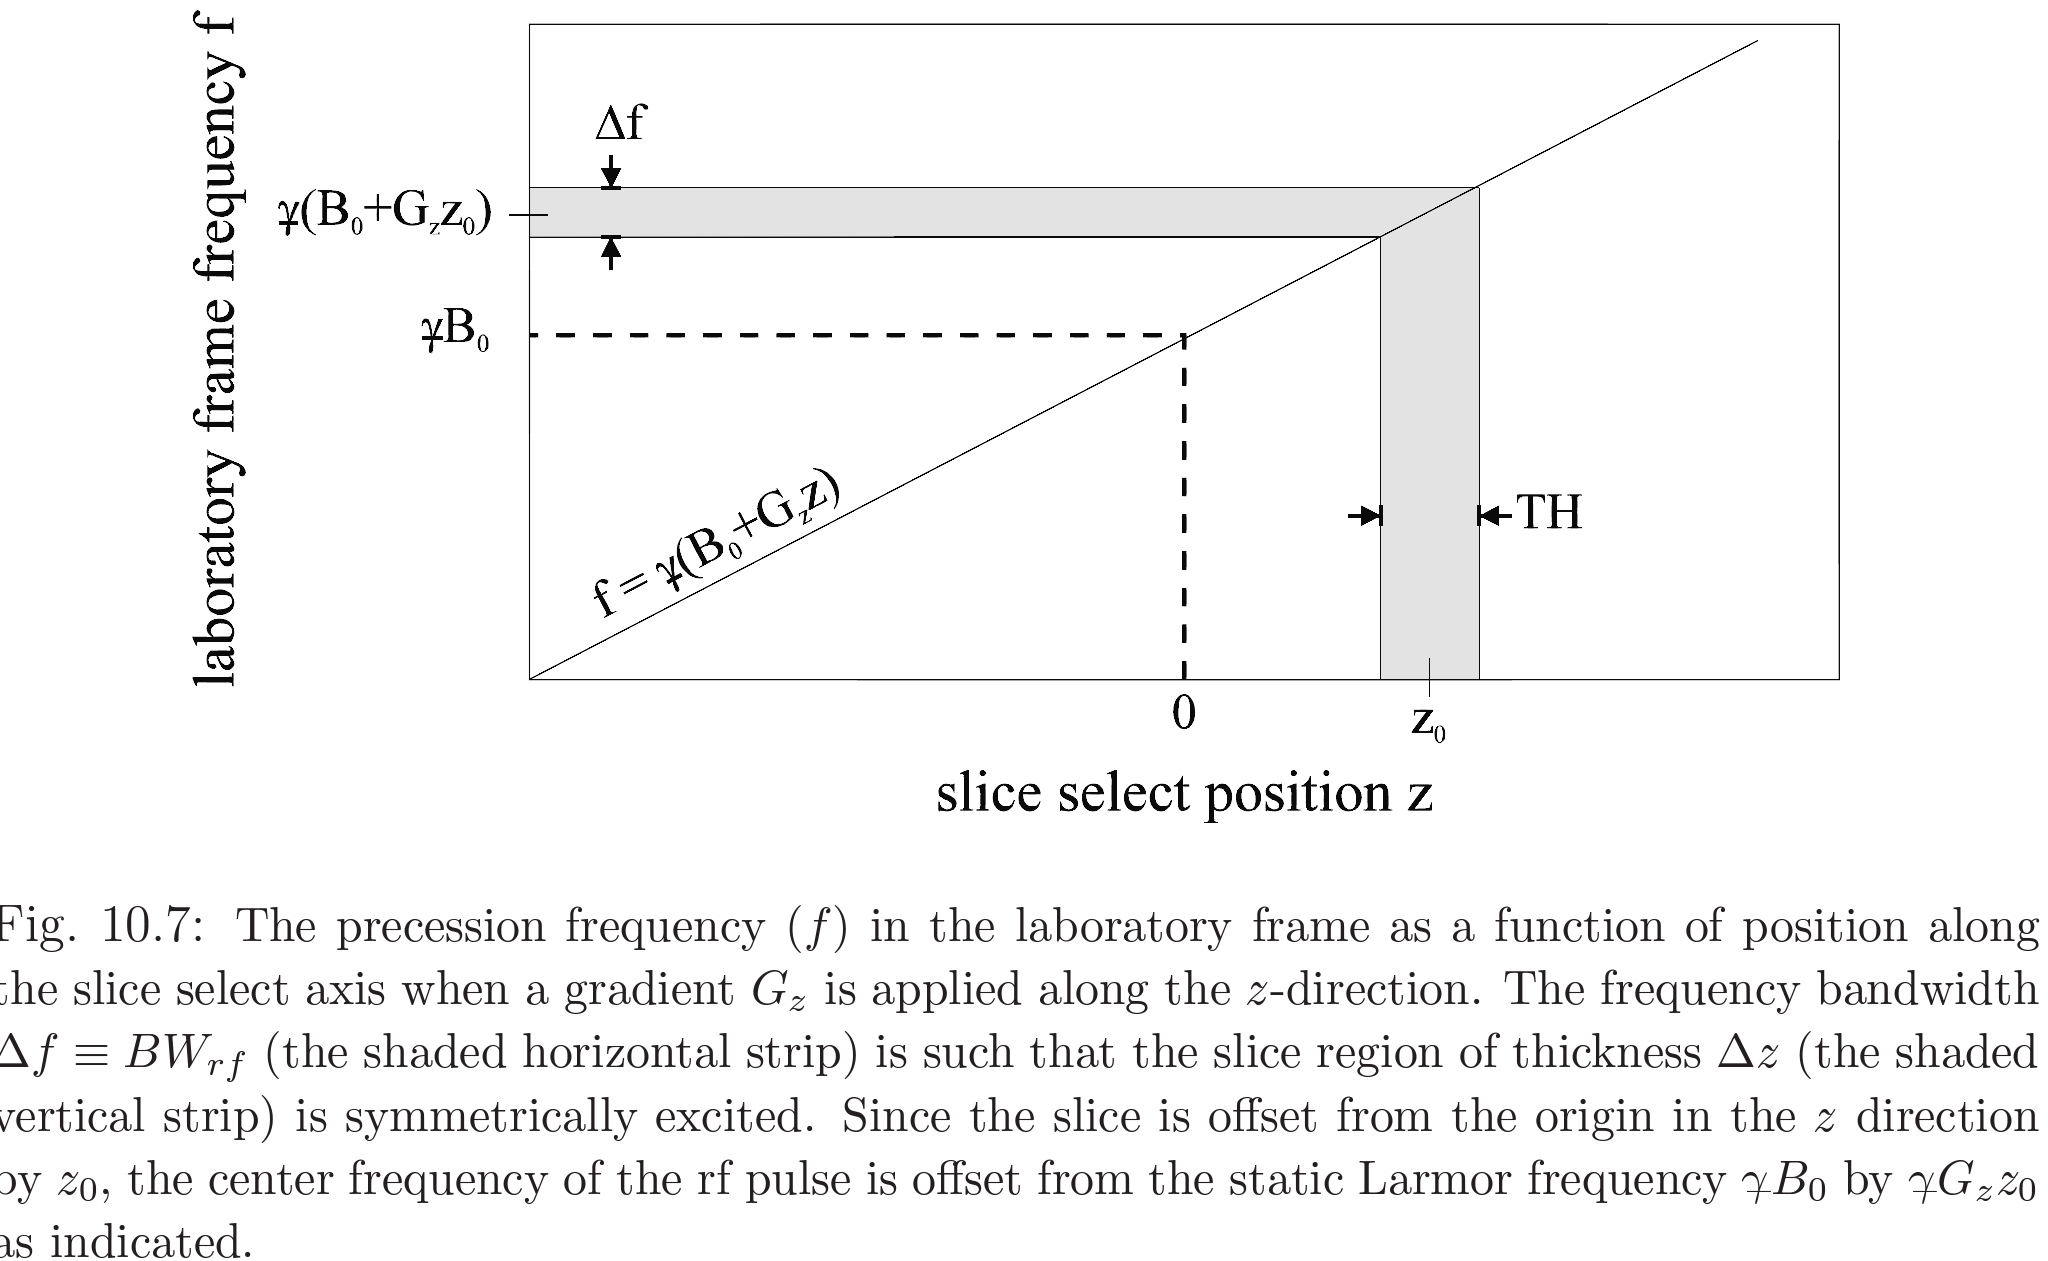
\includegraphics[trim={0cm 0cm 0 0},clip, keepaspectratio,width=0.3\textwidth]{sliceGBW}\label{fig:sliceGBW}\end{figure} 

Rephasing gradient: $\frac{|\int d tG_{rephase}|}{|\int d tG_{SS}|}=50\%$.

\begin{figure}[!ht]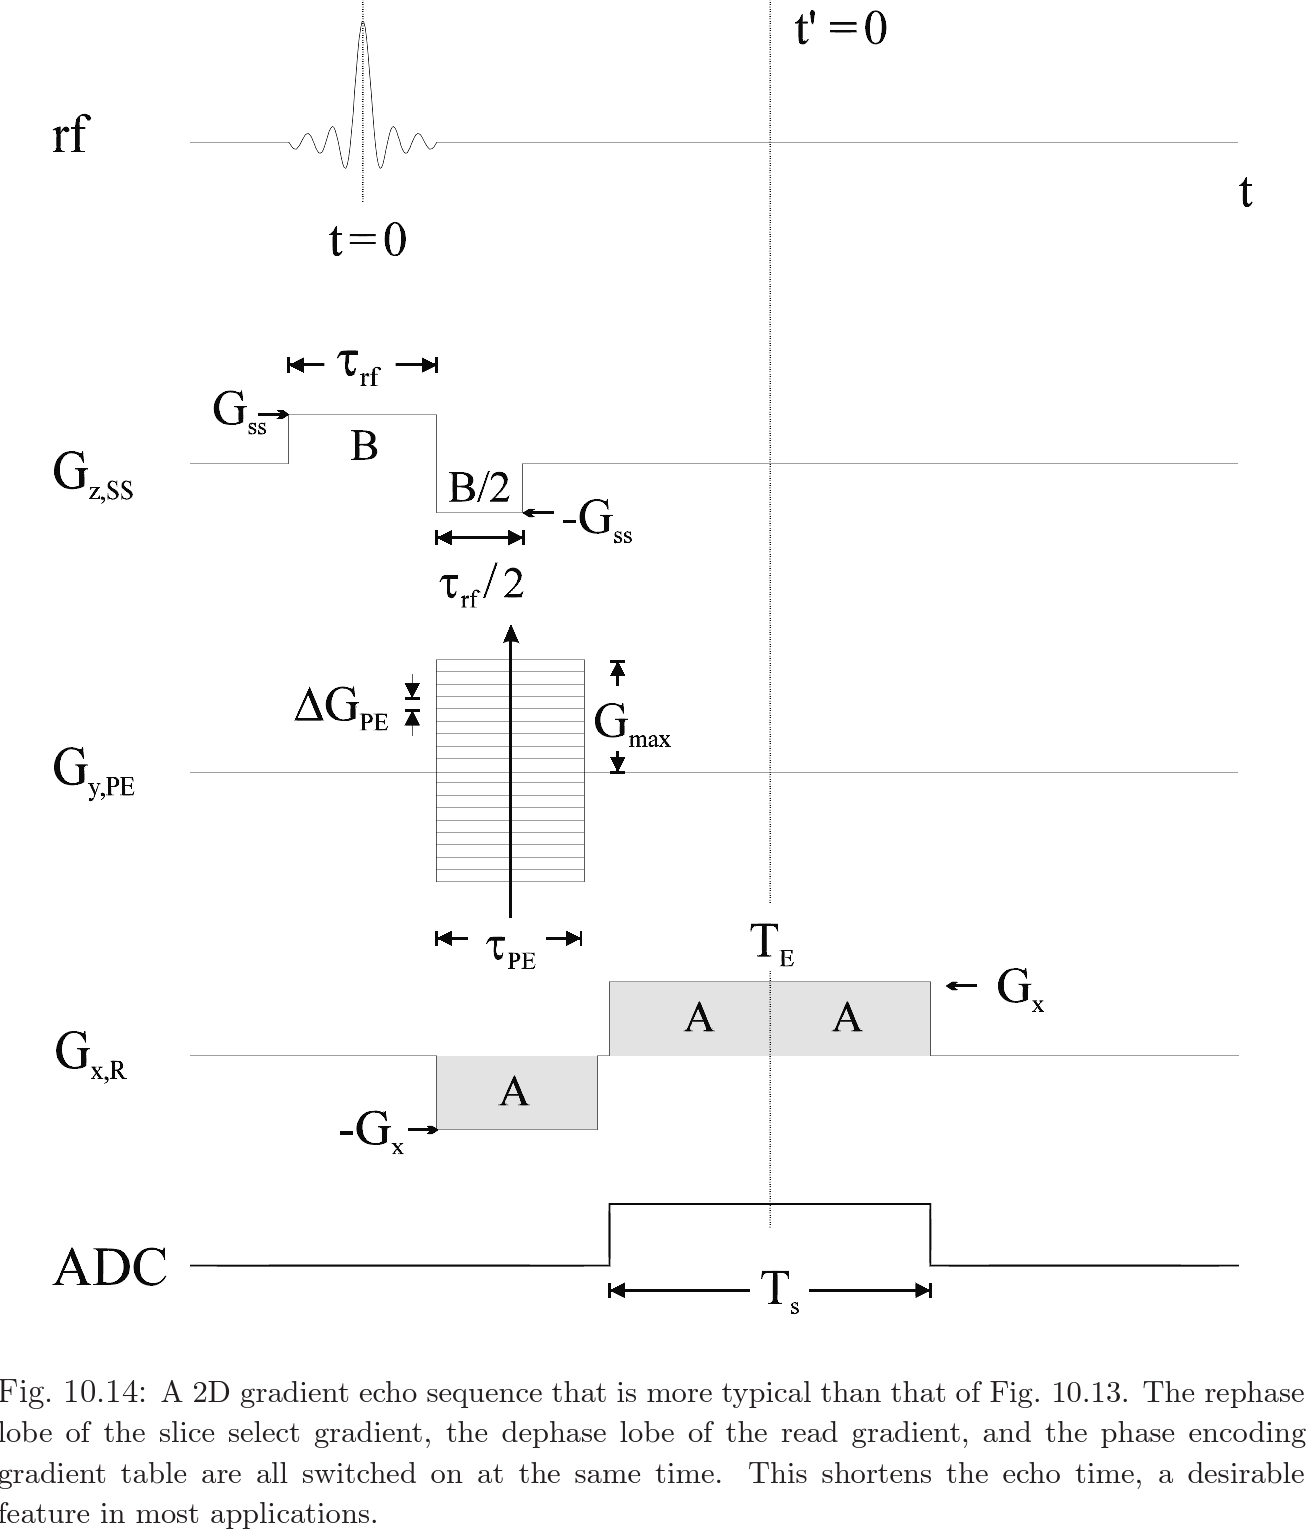
\includegraphics[trim={0cm 0cm 0 0},clip, keepaspectratio,width=0.4\textwidth]{sliceselection}\label{fig:sliceselection}\end{figure}

\end{block}
\end{frame}

\section{Filtering and resolution in Fourier T imaging}

\begin{frame}{Nyquist criterion and resolution}
$\frac{1}{\Delta k}=L=FOV$, A object size:
\begin{align*}
&\Delta k<\frac{1}{A}\\
&(\Delta k_R=\gammabar\int_t^{t+\Delta t}d t'G_R(t')=\frac{1}{L_R}<\frac{1}{A_R})\\
&f_R=BW_{read}=\frac{1}{\Delta t}=\gammabar G_RL_R>\gammabar G_RA_R
\end{align*}
Risoluzione: $\Delta x=\frac{1}{2n\Delta k}$, $k=(-n\Delta k,(n-1)\Delta k)$.
\end{frame}

\begin{frame}{FOV and spatial resolution}
    \begin{block}{Limited F imaging: partial k-space coverage}
    Time limitation restrict data sampled per readout ($N_x$), phase encoding ($N_y$) and partition encoding ($N_z$): reconstructed spin data for finite sampling $\hat{\rho}$.
    \begin{equation*}
        \rho(x)=\Delta k\sum_{p=-n}^{n-1}s(p\Delta k)\exp{i2\pi p\Delta k_x}
    \end{equation*}
    $W=2n\Delta k=$
    \end{block}
    \begin{block}{Aliasing (Nyquist criterion) and spatial resolution}
    To avoid aliasing $L=\FOV{}>A$: field of view $L=\invers{\Delta k}$ greater than object dimension.
    \end{block}
\begin{block}{Spatial resolution}
L'altra meta della trasformata di Fourier discreta
\begin{equation*}
s(k)=\Delta x\sum_{q=-n}^{n-1}\rho(q\Delta x)\exp{-i2\pi kq\Delta x}
\end{equation*}
Spatial resolution: $\Delta x=\frac{L}{N}=\frac{1}{N\Delta k}=\frac{1}{W}$ con $N=2n$.
\end{block}
\end{frame}

\begin{frame}{Filter and PSF}
A k-space filter $H(k)$ is a function that multiplies k-space MRI data, the F trasform is the associated PDF $h(x)$: $\rho(x)\to h(x)\circledast \rho(x)$.
\begin{block}{Continuus sampled truncated data}
\begin{align*}
&H_w(k)=\rect{(\frac{k+\Delta k/2}{W})}\\
&s_w(k)=s(k)H_w(k)
\end{align*}
\end{block}
\begin{block}{Gibbs ringing}
Fourier series repr. of function with steps
\end{block}
\begin{block}{Spatial resolution filter}
For arb. imaging method with PSF $h_{filter}(x)$ the spatial resolution is the area under the filter divide by $h(0)$:
\begin{equation*}
\Delta x_{filter}=\text{filter's blur}=\frac{1}{h_f(0)}\int d\,xh_f(x)=\frac{H_f(0)}{h_f(0)}
\end{equation*}
\end{block}
\end{frame}

\begin{frame}{$T_2^*$ decay effects}
When sampling time $T_s=\frac{2n\Delta k}{\gammabar|G|}$ is comparable to $T_2^*$ the exponential decay has filtering action on $s(k)$: filter model $\exp{-t'/T_2^*}$
\begin{equation*}
H_f(k)=\exp{-|k|/(\gammabar GT_2^*)}
\end{equation*}
approximable in most MRI cases ($\Delta k=\gammabar|G|\Delta t\ll\gammabar|G|T_2^*$):
\begin{equation*}
\Delta x_{T_2^*f}=\Delta x\frac{\alpha}{1-\exp{-\alpha}}
\end{equation*}
with $\alpha=\frac{T_s}{2T_2^*}$
\end{frame}

\section{Noise and contrast}\linkdest{noisecontrast}

\begin{frame}[allowframebreaks]{Signal and thermal noise}

\begin{block}{Segnale misurato}
Segnale misurato $s_m(k)$ somma $s_m(k)=s(k)+\epsilon(k)$ con funzione di autocorrelazione del rumor
\begin{equation*}
    R_{\epsilon}(\tau)=\exv{\epsilon(k_p)\epsilon^*{k_q}}|_{\tau=k_p-k_q}=\sigma_m^2\delta(\tau)
\end{equation*}
Rumore bianco distribuito normalmente con media 0 e varianza $\sigma_m^2$
\end{block}
\begin{block}{Noise in image domain}
\begin{align*}
&\eta(p\Delta x)=\frac{1}{N}\sum_{p'}\epsilon(p'\Delta k)\exp{i2\pi p'\Delta kp\Delta x}\\
&\var{(\eta(p\Delta x))}=\sigma_0^2(p\Delta x)=\frac{\sigma_m^2}{N}\\
&\rho_m(p\Delta x)=\rho_{m,0}(p\Delta x)+\eta(p\Delta x)\\
&\sigma_0^2(p\Delta x)|_{3D}=\frac{\sigma_m^2}{N_xN_yN_z}
\end{align*}
\end{block}
\end{frame}

\begin{frame}[allowframebreaks]{SNR and imaging parameters}
\begin{block}{Signal to Noise ratio and multi measures average}
k-space averaged sample
\begin{align*}
&s_{m,av}(k)=\frac{1}{N_{acq}}\sum_{i=1}^{N_a}s_{m,i}(k)\\
&\exv{s_{m,av}(k)}=s(k),\ \sigma_{m,av}(k)=\frac{\sigma_m(k)}{\sqrt{N_{acq}}}
\end{align*}
$\SNR{}$ of k-space signal and of given VXL:
\begin{align*}
&\SNR{(k)}=\frac{\exv{s_{m,av}(k)}}{\sigma_{m,av}(k)}=\sqrt{N_{acq}}\frac{s(k)}{\sigma_m(k)}\\
&\SNR{}/\VXL{}(p\Delta x, q\Delta y, r\Delta z)\propto\frac{\sqrt{N_{acq}}}{\sigma_0}
\end{align*}
\end{block}
\begin{block}{SNR and imaging parameters}
\begin{align*}
&\SNR{}/\VXL{}\propto\frac{\Delta x\Delta y\Delta z\sqrt{N_{acq}}}{\sqrt{\frac{\BWr{}}{N_xN_yN_z}}}\\
&\propto\Delta x\Delta y\Delta z\sqrt{N_{acq}N_xN_yN_z\Delta t}\\
&\Delta t= \frac{1}{\BW_{read}}=\frac{1}{L_x\gammabar G_x},\ T_s=N_x\Delta t\\
&\propto\Delta x\Delta y\Delta z\sqrt{N_{acq}N_xN_yN_zT_s}
\end{align*}
Degrading resolution to improve SNR.
\end{block}
\end{frame}

\begin{frame}{Contrasto}
    \begin{block}{Contrasto tessuto A/B}
\begin{align*}
&C_{AB}=S_A-S_B\\
&=\rho_{0A}(1-\exp{-\frac{T_R}{T_{1A}}})\exp{-\frac{T_E}{T*_{2A}}}-\rho_{0B}(1-\exp{-\frac{T_R}{T_{1B}}})\exp{-\frac{T_E}{T*_{2B}}}
\end{align*}
Spin density weighting:
\begin{equation*}
\left\{\begin{pmatrix}T_E\ll T_{2A,B}^*\\ T_R\gg T_{1A,B}\end{pmatrix}\right.\Rightarrow C_{AB}\approx\rho_{0A}-\rho_{0B}
\end{equation*}
$T_1$-weighting: $T_E\ll {T_2^*}_{AB}$.
$T_2^*$-weighting: $T_R\gg {T_1}_{AB}$.
\end{block}
\end{frame}

\section{FAt-Water separation}

\begin{wordonframe}{Fat-Water separation methods}
\begin{itemize}
    \item Chemical shift
    \item Selective excitation and tissue nulling
    \item Multiple point separation methods
\end{itemize}
\end{wordonframe}

\section{Random walks, relaxation and diffusion}

\begin{frame}{Molecular model for $T_2$}
Rapide fluttuazioni nel campo magnetico locale (pi\'u rapide di $\tau_L$): moto browniano, spin.
i-esimo spin \'e lungo $y'$: rapide fluttuazioni nel momento torcente determinano random walk di $\vec{\mu}_i$ sulla sfera unitaria. Distribuzione della fase gaussiana
\begin{equation*}
P(\phi)=\frac{\exp{-\phi^2/(2\exv{\phi_i^2})}}{\sqrt{2\pi\exv{\phi_i^2}}}    
\end{equation*}
e la componente trasversale $M_+$
\begin{equation*}
M_+=\frac{M_0}{\sqrt{2\pi\exv{\phi_i^2}}}\int d\,\phi\exp{i\phi}\exp{-\phi_i^2/(2\exv{\phi_i^2})}=M_0\exp{-\exv{\phi_i^2}/2}
\end{equation*}
\begin{block}{Brownian motion and $T_2$ signal loss}
Precession frequency of spin i around z is $\gamma B_{i,z}$: spin motion every $\tau_2$ and intrinsic B at j position
\begin{align*}
&\phi_i(N\tau_2)=\sum_j\gamma B_{i,z,j}\tau_2,\quad \exv{\phi_i^2(N\tau_2)}=\gamma^2\tau_2^2\sum_j\exv{B_{izj}^2}\to\frac{1}{3}\gamma^2\tau_2^2N\exv{B^2}\\
&M_+=M_0\exp{-\gamma^2\tau_2\exv{B^2}t/6},\quad T_2=\frac{6}{\gamma^2\tau_2\exv{B^2}}
\end{align*}
\end{block}
\end{frame}

\begin{frame}{Diffusion}
$x\to x+\epsilon_i\delta$ every $\tau_d$ seconds
\begin{align*}
&B(j\tau_d)=B(0)+G\delta\sum_i^j\epsilon_i\\
&\phi=-\sum^N\gamma\tau_d\Delta B(j\tau_d)=-G\delta\gamma\tau_d\sum_j^N\sum_i^j\epsilon_i\\
&M_+=M_0\exp{-\gamma^2 G^2\delta^2 t^3/(6\tau_d)}\to M_0\exp{-t/T_2}\exp{-\gamma^2 G^2Dt^3/3}
\end{align*}
\end{frame}

\part{NMR Spectroscopy}\linkdest{nmrspect}
\section{Nuclei in campi magnetici}

\begin{frame}{Spin nucleari}
    
\end{frame}


\begin{frame}{Momenti dipolo magnetico}
    $\frac{e\hbar}{2m_N}=\SI{3.1525e-8}{\ev\per\tesla}$, $\hbar=\SI{6.58e-16}{\ev\per\second}$, ($\gamma=\frac{g\mu_N}{\hbar}$)
\end{frame}

\begin{frame}{Precessione momento dipolo in campo magnetico}
   $\vec{\mu}=g\vec{l}\mu_N$, $\nu_{Lar}=\frac{\gamma B_0}{2\pi}$.
   Equazione di moto: $\TDy{t}{\vec{\mu}}=\vecp{\mu}{B}$.
(tab nucleispin $\gamma$: Nmr spectroscopypg10)
\end{frame}

\begin{frame}{Magnetizzazione del campione: longitudinal equilibrium magnetization}
Boltzmann distribution: $\frac{P(m=-1/2)}{P(m=+1/2)}=\exp{-\Delta E/kT}$, $\Delta E=\hbar\gamma B_0$: spin excess is $N\frac{\hbar\omega_0}{2kT}$ then $M_0=\rho_0\frac{\hbar^2\gamma^2}{4kT}B_0$
\end{frame}

\begin{frame}{Coordinate cartesiane}
\begin{columns}[T]
\begin{column}{0.5\textwidth}
\begin{align*}
&|d\vec{\mu}|=\mu\sin{\theta}|d\phi|\\
&|d\vec{\mu}|=\gamma|\vecp{\mu}{B}|\,dt=\gamma\mu B\sin{\theta}\,dt\\
&\Rightarrow\omega=|TDy{t}{\phi}|=\gamma B,\ \phi=-\omega_0t+\phi_0
\end{align*}
\end{column}
\begin{column}{0.5\textwidth}
\begin{align*}
&\mu_x(t)=\mu_x(0)\cos{\omega_0t}+\mu_y(0)\sin{\omega_0t}\\
&\mu_y(t)=\mu_y(0)\cos{\omega_0t}-\mu_x(0)\sin{\omega_0t}\\
&\mu_x(t)=\mu_z(0)\\
&\mu_+(t)=\mu_+(0)\exp{-i\omega_0t}
\end{align*}
\end{column}
\end{columns}

\end{frame}

\begin{frame}{Detecting system magnetization}
RF magnetic field at Larmor frequency rotate magnetization away from alignment with $B_0$:
\end{frame}

\begin{frame}{Precessione magnetizzazione: sistema di riferimento rotante}

\end{frame}

\begin{frame}{Precessione magnetizzazione: campo rotante}
   Rotating magnetic field:
   \begin{equation*}
   \vec{B}(t)=B_0\hat{z}+B_1(\hat{x}\cos{\omega t}-\hat{y}\sin{\omega t})
   \end{equation*}
\end{frame}

\section{NMR spectroscopy}

\begin{frame}{Chemical shift and other magnetic interactions}
\chemfig{**6(------)} \hspace{.5mm} + \hspace{.5mm} \chemfig{H_3C-Cl} \hspace{.5cm} $\xrightarrow{catalyst}$ \hspace{.5mm} \chemfig{**6(---(-)---)} \hspace{.5mm} + \hspace{.5mm} \chemfig{H-Cl}
\end{frame}

\begin{frame}{Aminoacidi}
Amin($NH_2$)-acido(COOH)-
\end{frame}

\begin{frame}{Benzene: aromatic shielding}
    
\end{frame}

\begin{frame}{Accoppiamento scalare}
    
\end{frame}

\part{ESR CW}\linkdest{ESRCW}
\input{ESRCW}

\part{Resonance revelation}\linkdest{Rrevelation}
\section{Tecniche di rivelazione}\linkdest{tech}

\begin{frame}{Classi di rivelatori}
\begin{itemize}
\item Passivo in onda continua: generatore separato dal circuito LC. Induzione di Bloch, Q-meter, metodi a ponte
\item Attivi in onda continua: il circuito risonante contenente il campione fa parte di un oscillatore la cui ampiezza varia al passaggio dalla risonanza. Marginale, Robinson.
\item Tecniche passive impulsive: inducono nel campione stati di magnetizzazione di non equilibrio per determinare i tempi di rilassamento (ritorno a equilibrio termodinamico).
\end{itemize}
\end{frame}

\subsection{CW NMR}

\begin{frame}{CW measurement}
\begin{columns}  \begin{column}{0.5\textwidth}
\begin{align*}
&I(t)=\frac{V_0\cos{\omega t+\phi}}{Z}\\
&Z=\sqrt{R^2+(X_L-X_C)^2}\ \phi=\arctan{\frac{X_L-X_C}{R}}\\
&V_C=X_CI=\frac{|V_0|}{\sqrt{\tau^2\omega^2+(\frac{\omega^2}{\omega_0^2}-1)^2}}\ \tau=RC
\end{align*}
\end{column} \begin{column}{0.5\textwidth}
Guadagno
\begin{align*}
&|G|^2=\frac{V_C^2}{V_0^2}\\
&=\frac{1}{(\frac{1}{Q})^2 \frac{\omega^2}{\omega_0^2}+(\frac{\omega^2}{\omega_0^2}-1)^2}\\
&=\frac{\omega_0^4}{\omega^2\delta^2+(\omega^2-\omega_0^2)^2}
\end{align*}
$\delta=R/L$ 
\end{column}  \end{columns}
$\chi(\omega)=\chi'+i\chi''$
\end{frame}

%\part{Basi NMR: nuclei, spin, campi magnetici e magnetizzazione della materia}\label{part:}
%\input{NMR}

\end{document}